%----------------------------------------------------------------------------------
% Exemplo do uso da classe tcc.cls. Veja o arquivo .cls
% para mais detalhes e instruções.
%----------------------------------------------------------------------------------

% Seleção de idioma da monografia. Por enquanto as únicas opções
% suportadas são 'portuguese' e 'english'
% Para impressão em frente e verso, use a opção 'twoside'. Da
% mesma forma, use 'oneside' para impressão em um lado apenas.
\documentclass[portuguese,oneside]{tcc}

%----------------------------------------------------------------
% Coloque seus pacotes abaixo.
%
% Obs.: muitos pacotes de uso comum do LaTeX, como amsmath,
% geometry e url já são automaticamente incluídos pela classe
% (veja o arquivo .cls). Isso torna obrigatória a presença destes
% no sistema para o uso desta classe, mas ao mesmo tempo o uso se
% torna mais simples.  Recomendo a instalação da versão mais
% recente da distribuição TeXLive (para Windows e UNIXes):
% www.tug.org/texlive/
%
% Pacotes e opções já incluídas automaticamente:
%
% \RequirePackage[T1]{fontenc}[2005/09/27]
% \RequirePackage[utf8x]{inputenc}[2008/03/30]
% \RequirePackage[english,brazil]{babel}[2008/07/06]
% \RequirePackage[a4paper]{geometry}[2010/09/12]
% \RequirePackage{textcomp}[2005/09/27]
% \RequirePackage{lmodern}[2009/10/30]
% \RequirePackage{indentfirst}[1995/11/23]
% \RequirePackage{setspace}[2000/12/01]
% \RequirePackage{textcase}[2004/10/07]
% \RequirePackage{float}[2001/11/08]
% \RequirePackage{amsmath}[2000/07/18]
% \RequirePackage{amssymb}[2009/06/22]
% \RequirePackage{amsfonts}[2009/06/22]
% \RequirePackage{url}
% \RequirePackage[table]{xcolor}[2007/01/21]
%----------------------------------------------------------------
% Para inserção de figuras.
\usepackage{graphicx}
% Utilize a opção 'pdftex' se você estiver usando o pdflatex (que
% permite figuras em formatos como .jpg ou .png)
%\usepackage[pdftex]{graphicx}

% Para centralizar o texto em uma célula de tabela (horizontalmente e verticalmente)
\usepackage{array}
\newcolumntype{P}[1]{>{\centering\arraybackslash}p{#1}}
\newcolumntype{M}[1]{>{\centering\arraybackslash}m{#1}}

% Para tabelas com elementos ocupando mais de uma linha
\usepackage{multirow}
% Para frações na mesma linha (ex. ⅓).
\usepackage{nicefrac}

% PACOTE DESATUALIZADO, USAR subcaption
% https://www.overleaf.com/learn/latex/Errors/Illegal_unit_of_measure_(pt_inserted)
% Para inserir figuras lado a lado.
%\usepackage{subfigure}
\usepackage{caption}
\usepackage{subcaption}

% Para formatar algoritmos.
% A opção [algo2e] é necessária para evitar conflitos
% com as definições da classe.
%\usepackage[algo2e]{algorithm2e}
\usepackage{algorithmic}
% Um float do tipo algoritmo. No momento
% este pacote é incompatível com a classe.
%\usepackage{algorithm}
% acronyms
\usepackage{acronym}

\usepackage[inline]{enumitem}

\newcommand{\ie}{{\it i.e.}}
\newcommand{\eg}{{\it e.g.}}
\newcommand{\etc}{{\it etc.}}
\newcommand{\etal}{{\it et al.}}

\newcommand{\R}{\mathbb{R}}
\newcommand{\vel}{$\vec{v}$~}
\newcommand{\pos}{$\vec{p}$~}
\newcommand{\A}{$\mathcal{A}$~}
\newcommand{\va}{$\vec{v_\mathcal{A}}$~}
\newcommand{\B}{$\mathcal{B}$~}
\newcommand{\vb}{$\vec{v_\mathcal{B}}$~}
\newcommand{\tcpa}{$t_{CPA}$~}
\newcommand{\dcpa}{$d_{CPA}$~}

\usepackage[normalem]{ulem}
\usepackage{todonotes}
\newcommand\frm[2][noinline]{\todo[author=FRM,color=red!75,size=tiny,#1]{{#2}}}
\newcommand{\correct}[3]{\sout{#1}{\color{red}#2}\frm{#3}}

\newcommand\fsa[2][noinline]{\todo[author=FSA,color=blue!40,size=tiny,#1]{{#2}}}
\newcommand{\comment}[3]{\sout{#1}{\color{blue}#2}\fsa{#3}}

%----------------------------------------------------------------
% Parâmetros customizados sob demanda
%----------------------------------------------------------------
\emergencystretch=1em   % Para evitar erro do tipo "overfull hbox"


%----------------------------------------------------------------
% Autor (OBRIGATÓRIO)
%----------------------------------------------------------------
\author{Felipe da Silva Angnes}

%----------------------------------------------------------------
% Título (OBRIGATÓRIO). Devem ser passados DOIS parâmetros,
% o título em português E o inglês, não importando o idioma
% escolhido. Os títulos são utilizados para a montagem da capa,
% resumo e abstract mais tarde.
%----------------------------------------------------------------
\title{Implementação do ponto de maior proximidade em um sistema compatível com COLREGS para Veículos de Superfície não Tripulados}
      {Closest Point of Approach implementation for a COLREGS compliant Unmanned Surface Vehicle system}

%----------------------------------------------------------------
% Opções para o tipo de trabalho (OBRIGATÓRIO)
%----------------------------------------------------------------
\tipotrabalho{\ptci}         % Proposta de Trabalho de Conclusão
%\tipotrabalho{\tci}         % Trabalho de Conclusão I
%\tipotrabalho{\tcii}        % Trabalho de Conclusão II

%----------------------------------------------------------------
% Seleção do curso ("este trabalho é um requisito parcial para
% obtenção do grau de (mestre ou doutor) em Ciência da Computação").
%----------------------------------------------------------------
%\curso{\cc} % Ciência da Computação
%\curso{\si} % Sistemas de Informação
%\curso{\es} % Engenharia de Software
\curso{\ec} %Engenharia de Computação

%----------------------------------------------------------------
% Orientador (e Co-orientador, caso haja um). É OBRIGATÓRIO
% informar pelo menos o orientador.
%----------------------------------------------------------------
\orientador{Felipe Meneguzzi}
%\coorientador{Ciclano de Farias}

%----------------------------------------------------------------
% A capa é inserida automaticamente. Por isso não é necessário
% chamar \maketitle
%----------------------------------------------------------------
\begin{document}

%----------------------------------------------------------------
% Depois da capa vem a dedicatória e a epígrafe.
%----------------------------------------------------------------
%\dedicatoria{Dedico este trabalho a meus pais.}

%\epigrafe{The art of simplicity is a puzzle of complexity.}
%         {Douglas Horton}

%----------------------------------------------------------------
% Também dá para fazer as duas na mesma página:
%----------------------------------------------------------------
%\dedigrafe{Dedico este trabalho a meus pais.}
%          {The art of simplicity is a puzzle of complexity.}
%          {Douglas Horton}

%----------------------------------------------------------------
% A seguir, a página de agradecimentos (OPCIONAL):
%----------------------------------------------------------------
% \begin{agradecimentos}
% À lorem ipsum, dolor sit amet consetetur sadipscing elitr sed diam
% nonumy eirmod tempor. invidunt ut labore et dolore magna aliquyam

% À erad sed, diam voluptua at vero, eos et accusam et justo duo
% dolores et ea rebum stet clita.

% À kasd gubergren, no sea. takimata sanctus est lorem ipsum dolor sit
% amet lorem ipsum dolor sit amet. consetetur sadipscing elitr sed

% À diam nonumy, eirmod tempor, invidunt ut labore et dolore magna
% aliquyam erat sed diam voluptua at.
% \end{agradecimentos}

%----------------------------------------------------------------
% Resumo, com as palavras-chave passadas por parâmetro
% (OBRIGATÓRIO, ao menos para teses e dissertações)
%----------------------------------------------------------------
\begin{resumo}{COLREGS, veículo de superfície não tripulado, evasão de colisão}
Uma embarcação que se move de forma autônoma é denominada Veículo de Superfície não Tripulado (do inglês \textit{"Unmanned Surface Vehicle"} - USV). O Regulamento de Colisão no Mar (do inglês \textit{"COLlision REGulations at Sea"} - COLREGS) define as regras para evitar colisões com embarcações que encontram outras embarcações. Posto isso, o principal objetivo desse trabalho é aprimorar um sistema para USV parcialmente compatível com COLREGS. A melhoria consiste em tornar o sistema USV capaz de determinar se os estados futuros das embarcações implicará em risco de colisão ou não. Essa identificação será realizada através da técnica do Ponto de Maior Proximidade (do inglês \textit{"Closest Point of Approach"} - CPA).
\end{resumo}

%----------------------------------------------------------------
% Abstract, com as palavras-chave passadas por parâmetro
% (OBRIGATÓRIO, ao menos para teses e dissertações)
%----------------------------------------------------------------
\begin{abstract}{COLREGS, unmanned surface vehicle, closest point of approach}
A vessel that moves autonomously is denominated an Unmanned Surface Vehicle (USV). The COLlision REGulations at Sea (COLREGS) defines the rules to avoid collision between vessels that finds each other. Set that, the main goal of this work is to improve an existent COLREGS partially compliant USV system. The improve consists in make the USV system able to determine if the vessels' future states will imply in a collision risk or not. The detection will be made through the Closest Point of Approach (CPA) technique.
\end{abstract}

%----------------------------------------------------------------
% Listas e sumário, nessa ordem. Somente o sumário é obrigatório,
% portanto, comente as outras listas, caso sejam desnecessárias.
%----------------------------------------------------------------
\listoffigures       % Lista de figuras      (OPCIONAL)

%\listoftables        % Lista de tabelas      (OPCIONAL)
%\listofalgorithms    % Lista de algoritmos   (OPCIONAL)
%\listofacronyms \frm{Está incompleta, tu usa muito mais siglas}      % Lista de siglas       (OPCIONAL)
%\listofabbreviations % Lista de abreviaturas (OPCIONAL)
%\listofsymbols       % Lista de símbolos     (OPCIONAL)
\tableofcontents     % Sumário               (OBRIGATÓRIO)

%----------------------------------------------------------------
% Aqui começa o desenvolvimento do trabalho. Para uma melhor
% organização do documento, separe-o em arquivos,
% um para cada capítulo. Para isso, utilize o comando \include,
% como mostrado abaixo.
%----------------------------------------------------------------
\begin{acronym}
\acro{COLREGS}  {COLlision REGulations at Sea}
\acro{CPA}      {Closest Point of Approach}
\acro{CRI}      {Collision Risk Index}
\acro{DCPA}     {Distance to Closest Point of Approach}
\acro{GNC}      {Guidance Navigation and Control}
\acro{IMO}      {International Marine Organization}
\acro{LSA}      {Laboratório de Sistemas Autônomos}
\acro{PUCRS}    {Pontifícia Universidade Católica do Rio Grande do Sul}
\acro{ROS}      {Robotic Operating System}
\acro{TCPA}     {Time to Closest Point of Approach}
\acro{USV}      {Unmanned Surface Vehicle}
\end{acronym}
%!TEX root = tcc_proposta.tex

%----------------------------------------------------------------------------------
% Exemplo do uso da classe tcc.cls. Veja o arquivo .cls
% para mais detalhes e instruções.
%----------------------------------------------------------------------------------

% PARA PREENCHIMENTO DO REVISOR:
% CHECKLIST
% [ ] Introduction: check the introduction 
    % [ ] Avoid jargon: Do you avoid jargon that is only explain in the rest of the text?
    % [ ] Clarity: Can anyone from computer science read the introduction and understand what's the objective?
    % [ ] Does it clearly describe the problem?
    % [ ] Does the introduction clearly state the contributions?

\chapter{Introdução}\label{chap1:intro}
	Nos últimos anos, avanços significativos em robótica e em inteligência artificial contribuíram para que pesquisas no desenvolvimento de veículos de superfície aquática não tripulados (do inglês \textit{"Unmanned Surface Vehicle"} - USV) ganhassem atenção~\cite{Huang2020Ship}. Um USV é definido por atuar de forma autônoma através de um sistema embarcado ou controlado remotamente~\cite{Song2018Two-level}. Conduzidas por frentes militares, científicas e privadas, pesquisas no desenvolvimento de USVs têm o intuito de auxiliar em atividades como monitoramento, comércio, exploração e pesquisas~\cite{Jurak2020COLREGS}. Caso realizadas por um USV, as atividades citadas poderiam possuir uma maior duração e potencialmente maior acurácia, além de permitir redução do custo de manutenção~\cite{Liu2016Unmanned}. Porém, aspirar essa série de atividades para um USV fará com que sua atuação ocorra em cenários compartilhados com outras embarcações~\cite{Kuwata2014Safe}.

    Sob responsabilidade da Organização Internacional da Marinha (do inglês \textit{"International Marine Organization"} - IMO), as regulamentações de prevenção de colisões no mar (do inglês \textit{"COLlision REGulations at Sea"} - COLREGS) definem como as embarcações devem agir em situações de colisão~\cite{Jurak2020COLREGS}. Visto que investigações apontam que acidentes marítimos acontecem principalmente pela violação das COLREGS~\cite{Song2018Two-level}, é importante considerar a sua implementação no desenvolvimento de USVs. Dada a frequência de colisões e a gravidade das consequências, acidentes entre embarcações são uma preocupação latente~\cite{Huang2019Generalized}. Por conta disso, evasão de colisão é um dos aspectos fundamentais no desenvolvimento de USV~\cite{Jurak2020COLREGS}. 

    Apesar da necessidade de considerar COLREGS no desenvolvimento de USVs, elas foram pensadas para serem compreendidas por humanos, que podem condicionar a sua aplicação à cada caso~\cite{Kuwata2014Safe}. Na Figura~\ref{fig:Kuwata2014_colregsInterpretation}, conforme apresentada por Kuwata \etal~\cite{Kuwata2014Safe}, é possível observar uma situação onde há risco de colisão (Figura~\ref{fig:Kuwata2014_colregApplicable}) e, portanto, deve-se aplicar as COLREGS. Uma situação semelhante porém sem risco de colisão é apresentada na Figura~\ref{fig:Kuwata2014_colregNA}, onde as COLREGS não são aplicáveis pois, dado a velocidade das embarcações, não há risco de colisão. Para identificar situações em que as COLREGS devem, ou não, ser aplicadas é preciso identificar que há um risco de colisão. Para isso, se utiliza um Índice de Risco de Colisão (do inglês \textit{"Collision Risk Index"} - CRI)~\cite{Huang2019Generalized}. Esse índice pode ser obtido através do método Ponto de Maior Aproximação (do inglês \textit{"Closest Point of Approach"} - CPA), que utiliza indicadores, como "tempo para o ponto de maior proximidade" (do inglês \textit{"Time to Closest Point of Approach"} - TCPA) e "distância no ponto de maior proximidade" (do inglês \textit{"Distance to Closest Point of Approach"} - DCPA), para determinar se um determinado encontro apresenta risco de colisão ou não~\cite{Huang2020Ship}. 
    
    Este trabalho apresenta o desenvolvimento do CPA em um sistema base para USV desenvolvido por Jurak~\cite{Jurak2020COLREGS}. O presente documento está estruturado da seguinte forma: no Capítulo~\ref{chap2:fund_teo} apresentamos a metodologia, os conceitos e as técnicas utilizadas neste trabalho; no Capítulo~\ref{chap3:framework_desenvolvimento} introduzimos as ferramentas utilizadas no desenvolvimento deste trabalho, bem como uma descrição do sistema base desenvolvido por Jurak~\cite{Jurak2020COLREGS}; 
    no Capítulo~\ref{chap4:desenvolvimento} apresentamos o desenvolvimento; no Capítulo~\ref{chap5:resultados} apresentamos as análises dos resultados obtidos nos testes realizados, bem como uma comparação com os resultados do sistema base; no Capítulo~\ref{chap6:conclusao} discutimos os resultados obtidos e dissertamos a respeito dos trabalhos futuros.
    
    \begin{figure}
		\centering
        \begin{subfigure}{0.4\textwidth}
            \centering
            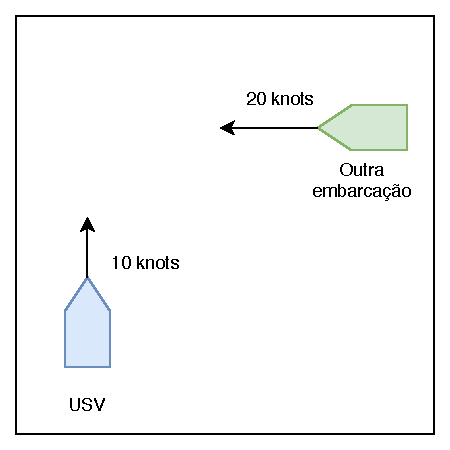
\includegraphics[width=\textwidth]{fig/chap1/kuwata_image_collision.pdf}
            \caption{}
            \label{fig:Kuwata2014_colregApplicable}
        \end{subfigure}
        \begin{subfigure}{0.4\textwidth}
            \centering
            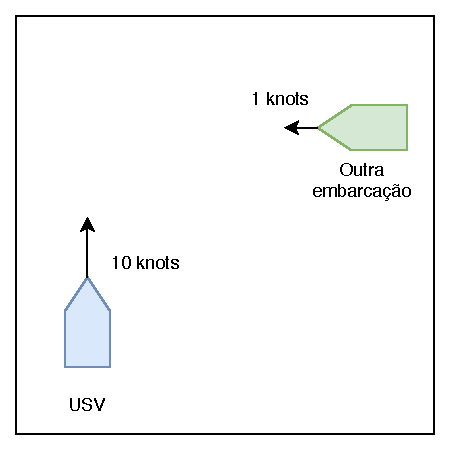
\includegraphics[width=\textwidth]{fig/chap1/kuwata_image_safe.pdf}
            \caption{}
            \label{fig:Kuwata2014_colregNA}
        \end{subfigure}
    
    \caption{Mesmo encontro para diferentes velocidades da embarcação que se aproxima. Na Figura~(a) a COLREGS é aplicável e o USV deve desviar da embarcação que se aproxima, enquanto que na Figura (b) a COLREGS não é aplicável e o USV pode seguir sua rota sem alteração.}
    \label{fig:Kuwata2014_colregsInterpretation}
    \end{figure}
%!TEX root = tcc_proposta.tex
%----------------------------------------------------------------------------------
% Exemplo do uso da classe tcc.cls. Veja o arquivo .cls
% para mais detalhes e instruções.
%----------------------------------------------------------------------------------

%[ ] Literature Review: the literature review is meant to convey your knowledge of the subject matter of the proposal, so check for
    %[ ] Does it provide basic definitions of the area?
    %[ ] Terminology dropping from the sky: new technical terms must be explained before they are used, avoid talk about a deteronic frombotzer if you have not said what this is
    %[ ] Consistency of terminology: do not use different terms to refer to the same technical entity, once you define something as X always refer to it as X
    %[ ] Are the references up to date: i.e. do you cite work that was published in the last 5-10 years


\chapter{Fundamentação Teórica}\label{chap2:fund_teo}
    Antes de entender o trabalho desenvolvido, é importante que se explique os principais conceitos técnicos que servem de base para o desenvolvimento deste trabalho. Para tanto, descrevemos a metodologia utilizada para guiar nossa pesquisa, o que é um veículo de superfície não tripulado, as regulamentações de prevenção de colisões no mar, como realizar a evasão de colisão, e como se determina a identificação do ponto de maior aproximação.
    
    
    \section{Metodologia}
       Este trabalho foi realizado seguindo a seguinte metodologia: 
        
        \begin{enumerate}[label=\alph*)]
            \item \textbf{Identificação de um Problema de Pesquisa}: a partir da análise do trabalho de Jurak~\cite{Jurak2020COLREGS} foi possível observar que evasão de colisão aplicado a USV é uma demanda atual, e que determinar se um encontro entre duas embarcações resultará em colisão é uma necessidade em sistemas para USV. Com isso, originou-se a seguinte pergunta de pesquisa:
            
            \vspace{3mm}
            
            \centerline{\textit{"Como identificar situações de colisões no âmbito de USVs?"}}
            
            \item \textbf{Definição da Sentença de Busca}: a partir da pergunta formulada na etapa anterior, obteve-se o entendimento de quais áreas seriam permeadas para respondê-la. Com esse entendimento, extraiu-se as palavras chaves formulando a seguinte sentença de busca:
            
            \vspace{3mm}
            
            \centerline{\textit{"USV" AND "COLREGS" AND "collision avoidance"}}
            
            \item \textbf{Seleção de Trabalhos Relacionados}: aplicando a sentença de busca definida em bases de busca como IEEE Explorer\footnote{https://ieeexplore.ieee.org/Xplore/home.jsp}, Scopus\footnote{https://www.scopus.com/search/form.uri?display=basic} e Science Direct\footnote{https://www.sciencedirect.com/}, foi realizada uma pré-seleção de trabalhos que poderiam embasar o trabalho a ser realizado. A pré-seleção foi feita com base na leitura do resumo (\textit{"abstract"}) do trabalho e da dissertação acerca de evasão de colisão e CPA, resultando em 28 trabalhos pré-selecionados. Posteriormente, através de uma análise mais detalhada dos trabalhos, para identificar as técnicas utilizadas, e considerando seus respectivos Índice H, foram selecionados os 5 trabalhos mais relevantes que foram utilizados como referência neste trabalho.
            
            \item \textbf{Leitura dos Trabalhos Selecionados e Extração de Conhecimentos Relevantes}: para obter um conhecimento mais aprofundado a respeito da área, do problema e das técnicas utilizadas pelos autores atualmente, foi realizada a leitura completa dos trabalhos atentando para a fundamentação teórica e analisando brevemente seus resultados. Com isso foi possível compreender como implementar CPA e quais resultados esperar da implementação.
            
            \item \textbf{Estruturação da Proposta de Trabalho}: com o conhecimento obtido da etapa anterior foi possível estruturar uma proposta de trabalho contendo uma contextualização, embasamento teórico, objetivos e os meios que serão utilizados para atingi-los.
            
            \item \textbf{Implementação da Proposta Aceita}: com a proposta analisada e aprovada pelos avaliadores, realizou-se a implementação do CPA e a integração com o sistema desenvolvido por Jurak~\cite{Jurak2020COLREGS}.
            
            \item \textbf{Execução Casos de Testes}: realizamos a validação da nossa implementação através de simulação, onde realizamos os mesmos casos de testes executados por Jurak~\cite{Jurak2020COLREGS} com a finalidade de verificar o impacto de nossa implementação no sistema base. Além disso, realizamos casos de testes específicos onde buscamos evidenciar nossa contribuição.
            
            \item \textbf{Análise dos Resultados}: analisamos o comportamento obtido na fase de testes e comparamos com o comportamento anterior à implementação deste trabalho.
        \end{enumerate}
    
    \section{Veículo de Superfície Não Tripulado}\label{subchap2:USV}
        Um veículo de superfície não tripulado (do inglês \textit{"Unmanned Surface Vehicle"} - USV) é caracterizado por realizar atividades navais de forma autônoma, ou controlado remotamente, sem a presença de tripulação~\cite{Liu2016Unmanned}. Tais características também enquadram um USV na categoria de um robô~\cite{Jurak2020COLREGS}.
        De acordo com Liu \etal~\cite{Liu2016Unmanned}, um USV pode ter as mais variadas aparências e funcionalidades, porém os seguintes componentes básicos devem compor um USV: 
        \begin{enumerate*}[label=\alph*)]
            \item casco e estruturas mecânicas auxiliares;
            \item sistema de propulsão;
            \item sistema de orientação, navegação e controle (do inglês \textit{"Guidance Navigation and Control"} - GNC);
            \item sistema de comunicação;
            \item equipamento de coleta de dados;
            \item estação de solo.
        \end{enumerate*}
        
        Dentre os elementos listados o sistema GNC é fundamental para automatizar uma embarcação, pois ele controlará a embarcação como um todo. Segundo Fossen~\cite{Fossen2011Handbook}, um sistema GNC consiste em controlar automaticamente ou remotamente dispositivos ou veículos. Sua função consiste em coletar informações a respeito da embarcação e seu entorno (\textit{Navigation}), gerenciar dados de missão encontrando o caminho necessário para completá-la (\textit{Guidance}) e executar as ações necessárias para atingir o objetivo desejado (\textit{Control})~\cite{Liu2016Unmanned}. A Figura ~\ref{fig:Liu2016_gncSystem}, criada com base em Liu \etal~\cite{Liu2016Unmanned}, mostra o sistema GNC de forma simplificada, apontando algumas de suas funcionalidades. Tais funções serão brevemente explicadas a seguir.
        
        \begin{figure}
            \centering
            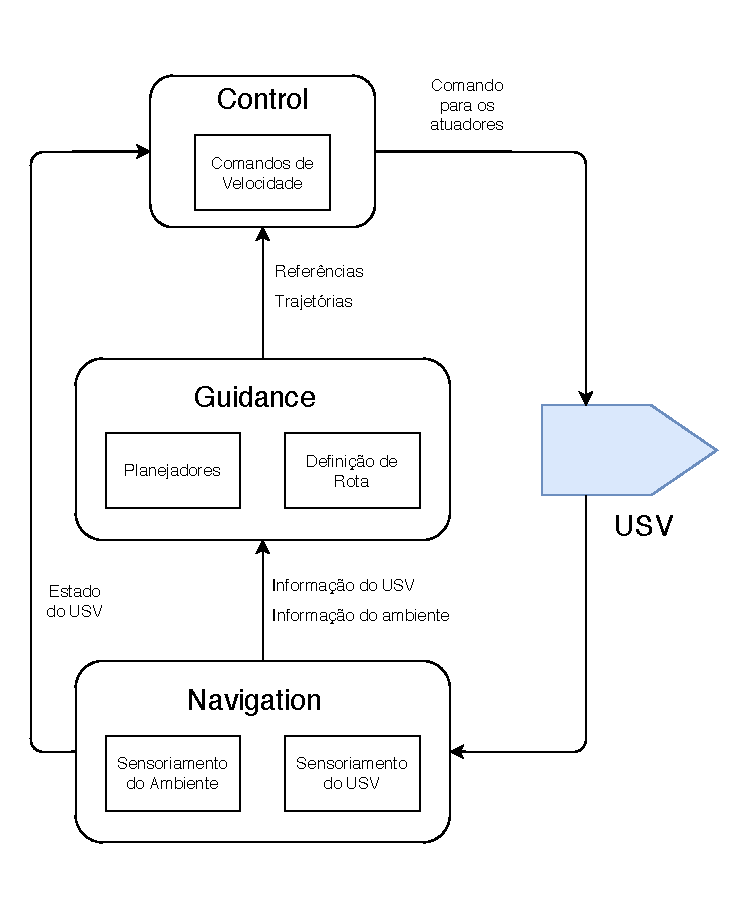
\includegraphics[width=0.8\textwidth]{fig/chap2/sistema_gnc_liu.pdf}
            \caption{Detalhamento do sistema GNC com suas respectivas funções (Imagem baseada em Liu~\etal~\cite{Liu2016Unmanned}).}
            \label{fig:Liu2016_gncSystem}
        \end{figure}
        
        \begin{enumerate}
            \item \textit{"Navigation":} subsistema responsável pela coleta de informações a respeito do barco (posição, velocidade, \etc) e seu entorno (obstáculos estáticos e obstáculos móveis). Essas informações são coletadas por meio de sensores, radares, câmeras, cartas náuticas e mapas. Os dados coletados são enviados para o subsistema \textit{"Guidance"} e \textit{"Control"}.
            
            \item \textit{"Guidance":} subsistema responsável por gerenciar os dados da missão atual a ser executada e definir os meios necessários para cumpri-la. Através dos dados obtidos do subsistema \textit{"Navigation"}, as ações necessárias para atingir o objetivo são definidas e enviadas para o subsistema \textit{"Control"}.
            
            \item \textit{"Control":} subsistema que, com base no estado atual da embarcação obtido pelo subsistema \textit{"Navigation"}, gera os comandos necessários para realizar as ações definidas pelo subsistema \textit{"Guidance"}. Além disso, também é sua responsabilidade executar os comandos gerados diretamente nos atuadores da embarcação.
        \end{enumerate}
        
        Visto que o escopo de desenvolvimento deste trabalho é em evasão de colisão, focaremos no subsistema responsável por tal função: o subsistema de \textit{"Guidance"}. Sua implementação consiste em, além do gerenciamento dos dados de missão, estabelecer qual a melhor rota para o USV percorrer~\cite{Jurak2020COLREGS}. A definição da rota geralmente ocorre em dois níveis: global e local. Ambos os níveis utilizam planejadores; o planejador global definirá a rota a ser corrida em um mapa de larga escala, chamada de rota global, considerando obstáculos estáticos conhecidos; já o planejador local atentará para o surgimento de obstáculos que não foram considerados na rota global e que precisarão ser desviados, desviando da rota global momentaneamente através de uma rota local específica para a atual situação~\cite{Liu2016Unmanned}.
    
    \section{Regulamentações de Prevenção de Colisões no Mar}\label{subchap2:colregs}
        Buscando padronizar as ações tomadas para evitar colisões, a Organização Internacional da Marinha (IMO - do inglês \textit{"International Marine Organization"}) definiu as regulamentações de prevenção de colisões no mar (COLREGS - do inglês \textit{"COLlision REGulations at Sea"})~\cite{COLREGS}.
        Para que o uso de USV não apresente perigo para outras embarcações, sendo elas tripuladas ou não, é necessário que ele realize ações conhecidas e esperadas pela embarcação que se aproxima. Sendo assim, o USV deverá realizar suas ações de acordo com as COLREGS de forma que seja perceptível para a outra embarcação~\cite{Kuwata2014Safe}. Jurak~\cite{Jurak2020COLREGS} em seu sistema considerou os encontros \textit{"head-on"}, \textit{"crossing from left"}, \textit{"crossing from right"} e \textit{"overtake"}. As situações listadas são ilustradas na Figura~\ref{fig:Jurak2020COLREGS_colregsSituations} e explicadas a seguir. 
        
        \begin{figure}
            \centering
            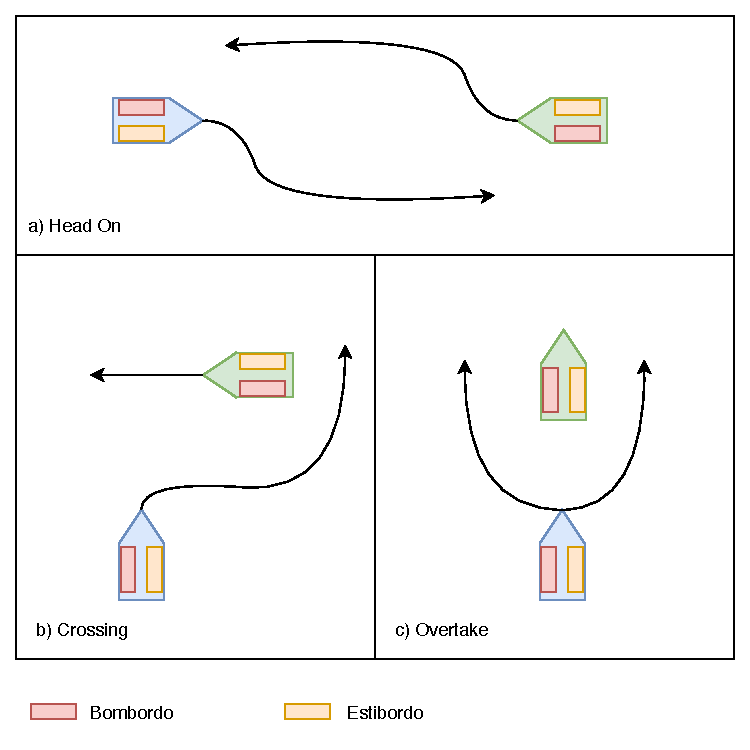
\includegraphics[width=\textwidth]{fig/chap2/encontros_colregs.pdf}
            \caption{Tipos de encontros entre embarcações previstos pelas COLREGS~\cite{Jurak2020COLREGS}.}
            \label{fig:Jurak2020COLREGS_colregsSituations}
        \end{figure}
        
        \begin{enumerate}[label=\alph*]
            \item \textit{"Head-on":} situação em que as embarcações se encontram frente a frente. Nesse caso, as COLREGS especificam que ambas as embarcações devem evitar a colisão virando à direita  (\textit{"starboard side"} - estibordo) e, por consequência, passando pelo lado esquerdo (\textit{"port side"} - bombordo) da outra embarcação.
            
            \item \textit{"Crossing from left/right":} situação em que uma embarcação cruzará o caminho da outra. Nesse caso, a embarcação que encontrar a outra no seu lado direito (\textit{"startboard side"} - estibordo) é responsável por evitar a colisão contornando a embarcação que se aproxima por trás, realizando uma conversão à direita (\textit{"startboard"} - estibordo). Já a embarcação que possuir a outra no seu lado esquerdo (\textit{"port side"} - bombordo), não deverá mudar seu curso.
            
            \item \textit{"Overtaking":} situação em que uma embarcação se encontra em uma velocidade maior do que a embarcação que se encontra à frente. Nesse caso a embarcação que se aproxima deve desviar pelo lado em que não causará uma nova situação de \textit{"overtaking"}.
        \end{enumerate}
    
    \section{Evasão de Colisão}\label{subchap2:prev_col}
        Uma tarefa primordial quando se trata de navegação é evitar que a embarcação colida com algum obstáculo e outras embarcações. Entretanto, prevenção de colisão consiste em um dos principais desafios ao desenvolver um USV~\cite{Jurak2020COLREGS}. Em um USV o sistema GNC é responsável por realizar todo o procedimento de prevenção de colisão, sendo o subsistema \textit{"Guidance"} o encarregado de detectar a colisão e encontrar uma solução para que ela não ocorra~\cite{Huang2020Ship}.
        Huang \etal~\cite[p.451]{Huang2020Ship} define prevenção de colisão como: \textit{"Prevenção de colisão é o processo em que uma embarcação desvia de sua trajetória planejada para evitar contato físico indesejado em um certo tempo futuro."} Com isso, Huang \etal~\cite{Huang2020Ship} separa o processo de prevenção de colisão nas seguintes etapas: 
        
        \begin{enumerate}
            \item \textbf{Previsão de Movimento}: que prevê estados futuros do USV e de todas as outras embarcações envolvidas no encontro;
            \item \textbf{Detecção de Conflito}: determina se o USV está em risco de colisão;
            \item \textbf{Resolução de Conflito}: encontrará o melhor caminho para evitar a colisão.
        \end{enumerate}
        
        A Figura~\ref{fig:Huang2020_collisionAvoidanceProcess}, feita com base em Huang \etal~\cite{Huang2020Ship}, mostra o fluxo de informação realizada em um sistema GNC no procedimento de prevenção de colisão. Na imagem, podemos considerar \textit{"Observer"} e \textit{"Actuator"} como módulos dos subsistemas de \textit{"Navigation"} e \textit{"Control"}, respectivamente. Os módulos envoltos pelo pontilhado vermelho correspondem às etapas listadas anteriormente e são de responsabilidade do subsistema \textit{"Guidance"}. As informações coletadas pelo \textit{"Observer"} são utilizadas pelo módulo \textit{"Motion Prediction"}, quando implementado, para realizar as previsões necessárias. O módulo \textit{"Conflict Detection"} utilizará as informações providas pelo \textit{"Motion Prediction"}, e/ou \textit{"Observer"}, a fim de identificar se há risco de colisão. Se não houver, as diretivas de caminho e velocidade são enviadas diretamente para o \textit{"Actuator"}. Caso haja risco de colisão, o módulo \textit{"Conflict Resolution"} será acionado para que encontre um caminho seguro para evitar a colisão, consequentemente, gerando diretivas de caminho e velocidade que levarão a um desvio momentâneo da rota global.
        
        \begin{figure}[H]
            \centering
            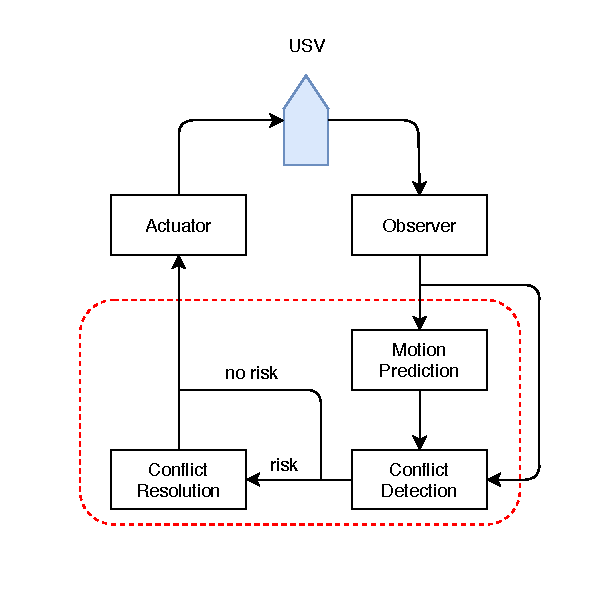
\includegraphics{fig/chap2/fluxo_de_informação.pdf}
            \caption{Fluxo de informação em um sistema GNC no procedimento de prevenção de colisão (Imagem baseada em Huang~\etal~\cite{Huang2020Ship}).}
            \label{fig:Huang2020_collisionAvoidanceProcess}
        \end{figure}
        
    \section{Ponto de Maior Aproximação}\label{subchap2:cpa}
        Um meio popular de se avaliar o Índice de Risco de Colisão (do inglês \textit{"Collision Risk Index"} - CRI) é através do método de Ponto de Maior Aproximação (do inglês \textit{"Closest Point of Approach"} -  CPA)~\cite{Huang2020Ship}. Nele, dois indicadores são considerados: Distância no ponto de maior aproximação (DCPA - do inglês \textit{"Distance to Closest Point of Approach"}), e Tempo para o Ponto de Maior Aproximação (TCPA - do inglês \textit{"Time to Closest Point of Approach"})~\cite{Huang2019Generalized}. Ambos indicadores são valores numéricos e contribuem para a detecção de uma situação de risco de colisão. Quando os valores resultantes atingirem um limiar (\textit{"threshold"}), é detectado um risco de colisão eminente e o procedimento para evitar o acidente é iniciado~\cite{Huang2020Ship}. 
        
        Segundo Kuwata~\etal~\cite{Kuwata2014Safe}, a partir da posição \pos e da velocidade \vel das embarcações é possível obter o \tcpa através da equação~\eqref{eq:tcpa}, e o \dcpa através da equação~\eqref{eq:dcpa}. Utilizaremos os indicadores \tcpa e \dcpa para identificar encontros em que a COLREGS deve ser aplicada. Se os valores obtidos satisfizerem a condição descrita na Desigualdade~\eqref{eq:cpaThreshold}, é preciso evadir da colisão de acordo com a COLREGS aplicável ao encontro~\cite{Kuwata2014Safe}. Para este trabalho consideramos $t_{max} = 20s$ e $d_{min} = 9m$.
        % Comentário para evitar novo parágrafo
        \begin{align}
            t_{\rm CPA} &=
            \begin{cases}
                0, & \text{if } \Vert\vec{v}_{A}-\vec{v}_{B}\Vert\leq\epsilon\\
                \displaystyle{{(\vec{p}_{A}-\vec{p}_{B})\cdot(\vec{v}_{A}-\vec{v}_{B})}\over{\Vert\vec{v}_{A}-\vec{v}_{B}\Vert^{2}}}
            \end{cases}\label{eq:tcpa}\\
            d_{\rm CPA} &=\bigl\Vert (\vec{p}_{A}+\vec{v}_{A}t_{\rm CPA})-(\vec{p}_{B}+\vec{v}_{B}t_{\rm CPA})\bigr\Vert\label{eq:dcpa}
        \end{align}
        
        \begin{equation}\label{eq:cpaThreshold}
            0\leq t_{\rm CPA}\leq t_{\max} \land d_{\rm CPA}\leq d_{\min}
        \end{equation}
    
        Para obter um maior entendimento de como é possível analisar os estados futuros das embarcações para avaliar o risco de colisão a partir da Equação~\ref{eq:tcpa}, explicaremos visualmente. Consideremos um USV cuja posição é $\vec{p}_{A}(1,1)$ e uma outra embarcação $\mathcal{B}$ cuja posição é $\vec{p}_{B}(7,1)$. Consideremos também que a velocidade do USV é $\vec{v}_{A}(1,1)$ e que a velocidade da embarcação $\mathcal{B}$ é $\vec{v}_{B}(-1,1)$, como mostrado na Figura~\ref{fig:chap2_scenario}.
        Primeiramente verifiquemos se $\Vert\vec{v}_{A}-\vec{v}_{B}\Vert\leq\epsilon$ e, caso a verificação seja verdadeira, consideraremos $t_{CPA} = 0$. Isso é para evitar que o denominador da Equação~\ref{eq:tcpa} resulte em um número muito pequeno, fazendo com que o \tcpa resulte em um número muito grande, além de garantir que não haverá uma divisão por zero. Porém neste caso temos que $\Vert\vec{v}_{A}-\vec{v}_{B}\Vert = 4$, logo, podemos calcular o \tcpa de acordo com o segundo caso da Equação~\ref{eq:tcpa}. Calculando a posição e a velocidade relativa das embarcações temos que $\vec{p}_{A}-\vec{p}_{B} = (-6,0)$ e que $\vec{v}_{A}-\vec{v}_{B} = (2,0)$, respectivamente. Essas operações são ilustradas pela Figura~\ref{fig:chap2_pa_pb} e pela Figura~\ref{fig:chap2_va_vb}, respectivamente. Com os vetores resultantes podemos realizar o produto escalar $(-6,0)\cdot(2,0) = -12$, que aplicado na Equação~\ref{eq:tcpa} resulta em $t_{CPA} = -3$.
    
        \begin{figure}[H]
            \centering
            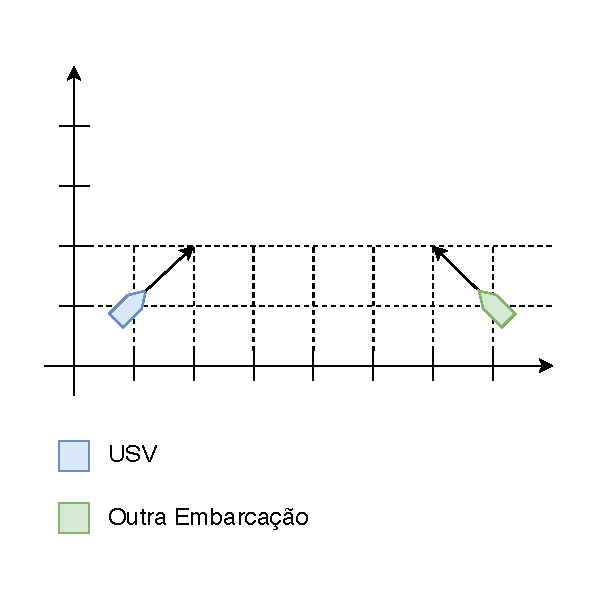
\includegraphics{fig/chap2/cpa_example_scenario.pdf}
            \caption{Cenário inicial do exemplo apresentado.}
            \label{fig:chap2_scenario}
        \end{figure}
        
        \begin{figure}
            \centering
            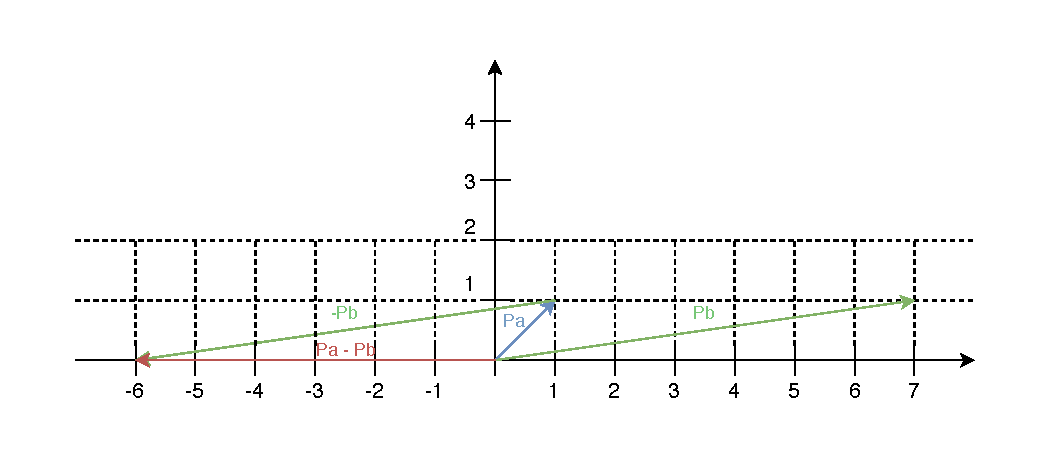
\includegraphics{fig/chap2/cpa_explanation_pa_pb.pdf}
            \caption{Operação vetorial $\vec{p}_{A}-\vec{p}_{B}$}
            \label{fig:chap2_pa_pb}
        \end{figure}
        
        \begin{figure}
            \centering
            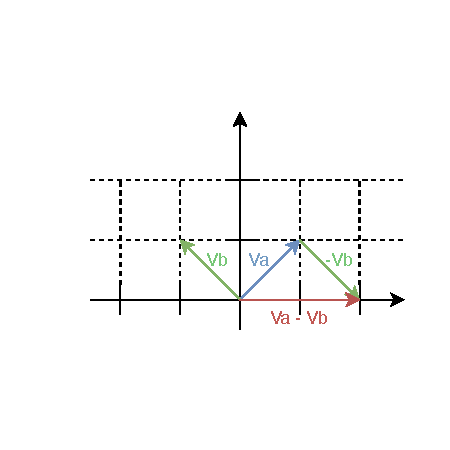
\includegraphics[scale=1.5]{fig/chap2/cpa_explanation_va_vb.pdf}
            \caption{Operação vetorial  $\vec{v}_{A}-\vec{v}_{B}$}
            \label{fig:chap2_va_vb}
        \end{figure}
        
        Com o \tcpa calculado, podemos obter o \dcpa. A Equação~\ref{eq:dcpa} coloca que os vetores velocidade das embarcações devem ser multiplicados pelo \tcpa encontrado. Apesar de Kuwata~\etal~\cite{Kuwata2014Safe} não indicar explicitamente o uso do valor absoluto do \tcpa encontrado, optamos por fazê-lo dado que se multiplicássemos as velocidades por um \tcpa negativo, estaríamos invertendo o sentido das velocidades, o que não é desejável, dado que o \tcpa é utilizado no cálculo do \dcpa para estender o vetor velocidade da embarcação, partindo da sua posição, até o ponto de maior proximidade. Posto isso, ao aplicarmos a Equação~\ref{eq:dcpa} para ambas as embarcações, temos os pontos em que cada uma delas estarão no momento em que estiverem mais próximas uma da outra, para que seja calculada a distância entre elas. 
      
        Para ilustrar o cálculo do \dcpa, daremos continuidade ao exemplo apresentado até então. Aplicando os vetores posição e os vetores velocidade das embarcações, já multiplicados pelo valor absoluto do \tcpa, na Equação~\ref{eq:dcpa} temos que $\Vert (1+3,1+3)-(7-3,1+3)\Vert = 0$. Essa é a distância entre as embarcações no ponto de maior proximidade, ou seja, certamente haverá colisão. Na Figura~\ref{fig:chap2_collision} apresentamos as embarcações em suas posições iniciais e estendemos o vetor velocidade \tcpa vezes, indicando onde cada embarcação estaria em cada instante de tempo. É possível observar que no terceiro instante de tempo as embarcações estariam ocupando a mesma posição, ou seja, a distância entre elas seria zero.
        
        \begin{figure}[H]
            \centering
            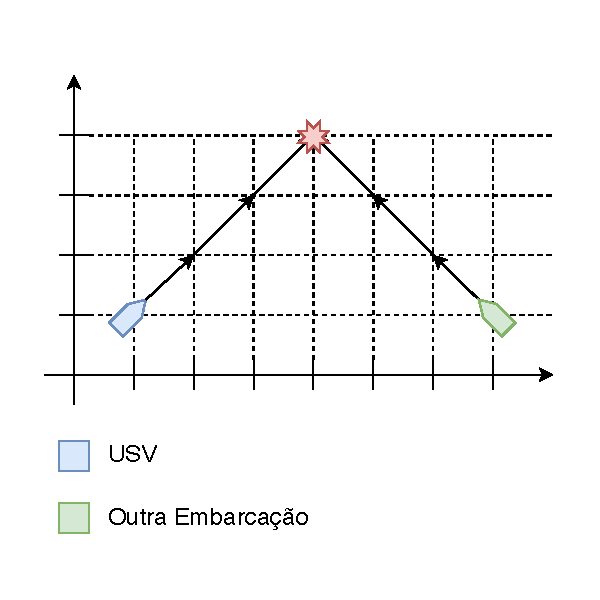
\includegraphics{fig/chap2/cpa_explanation_collision.pdf}
            \caption{Ilustração do CPA calculado - Exemplo 1}
            \label{fig:chap2_collision}
        \end{figure}
        
        Em um segundo exemplo, consideremos as mesmas condições iniciais do exemplo anterior alterando apenas a velocidade da outra embarcação para $\vec{v}_{B}(-0.5,-0.5)$. Nesse caso, realizando os mesmos cálculos, temos que $t_{CPA} = 3.6s$ e $d_{CPA} = 1.9m$. Isso significa que no ponto de maior proximidade a distância entre as embarcações será de 1.9m. A Figura~\ref{fig:chap2_almost_collision} apresenta informações 
        análogas à Figura~\ref{fig:chap2_collision}, com a única diferença sendo o ponto azul indicando a posição do USV no tempo t = \tcpa e o ponto verde indicando a posição da outra embarcação no tempo t = \tcpa. Com essas informações, é possível determinar se essa é uma 
        situação de risco ou não. Se for uma situação de risco é necessário evadir de acordo com as COLREGS, caso contrário a evasão não é necessária.
        
        \begin{figure}
            \centering
            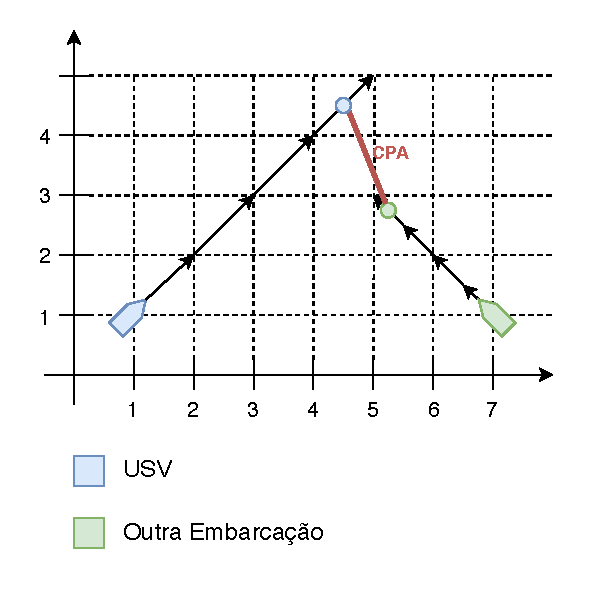
\includegraphics{fig/chap2/cpa_explanation_almost_collision.pdf}
            \caption{Ilustração do CPA calculado - Exemplo 2}
            \label{fig:chap2_almost_collision}
        \end{figure} 
%!TEX root = tcc_final.tex
\chapter{Framework de Desenvolvimento}\label{chap3:framework_desenvolvimento}
    
    % Referência para este capítulo é a própria documentação do ROS: http://wiki.ros.org/
    % Paper sobre ROS (não foi usado como referência, botei aqui apenas para manter o link): http://www.robotics.stanford.edu/~ang/papers/icraoss09-ROS.pdf
    
    Neste capítulo serão apresentadas as ferramentas utilizadas para o desenvolvimento deste trabalho, as funcionalidades que foram exploradas de cada uma delas e também detalhes importantes para o entendimento do desenvolvimento do trabalho.
    
    \section{Robot Operating System - ROS} \label{subchap3:ros}
        O sistema operacional robótico (do inglês \textit{"Robot Operating System"} - ROS) é um meta sistema operacional de código aberto mantido pelos esforços da comunidade internacional de pesquisadores em robótica. Um meta sistema operacional é um sistema que provê funcionalidades características de um sistema operacional porém é hospedado e executado pelo sistema operacional existente na máquina em questão.
        O ROS possui funcionalidades como abstração de hardware, controle de periféricos, troca de mensagens entre processos e etc, porém não possui autonomia sobre escalonamento, gerenciamento de memória e demais atividades que ficam a cargo do sistema operacional hospedeiro. O ROS pode ser compreendido como uma rede de processos (nodos) que possuem algum fator de acoplamento. Esses nodos podem ser processados na mesma máquina ou em máquinas distintas. A comunicação entre esses nodos é realizada 
        através da infraestrutura fornecida pelo ROS, que contempla comunicação síncrona e assíncrona. Os principais conceitos do ROS necessários para o entendimento deste trabalho são explicados a seguir:
        
        \begin{enumerate}[label=\Alph*]
            \item \textbf{Pacotes:} conjunto de nodos, bibliotecas, arquivos de configuração e etc que pode ser distribuído e integrado em sistemas distintos;
            \item \textbf{Nodos:} são os processos que formam o pacote. Cada processo pode ser um executável ou então um executável pode conter múltiplos processos.
            \item \textbf{Tópicos:} funcionalidade oferecida pelo ROS para troca de mensagens em uma abordagem publicador/inscrito (do inglês \textit{publisher/subscriber}). Comunicação N para N onde publicadores disponibilizam uma informação no tópico para possível consumo dos inscritos. Comunicação ocorre de forma não bloqueante, caracterizando uma comunicação assíncrona. % Encontrar referência para comunicação não bloqueante = assíncrona
            \item \textbf{Serviços:} funcionalidade oferecida pelo ROS para troca de mensagens em uma abordagem requisição e resposta. Essa comunicação ocorre de forma bloqueante, caracterizando uma comunicação síncrona. % Encontrar referência para comunicação bloqueante = síncrona
            \item \textbf{Bags:} formato do arquivo utilizando pelo ROS para gravar informações publicadas nos tópicos pelos nodos. Eficaz ferramenta para análise de execuções realizadas.
        \end{enumerate}
    
        
    
    \section{Sistema Base} \label{subchap3:sistema_base}
        O desenvolvimento deste trabalho foi realizado a partir do sistema implementado por Jurak~\cite{Jurak2020COLREGS}, que consiste em um sistema autônomo para veículos não tripulados que navegam na superfície da água (do inglês \textit{"Unmanned Surface Vehicle"} - USV) em conformidade com as regulamentações de prevenção de colisões no mar (do inglês \textit{"COLlision REGulations at Sea"} - COLREGS)~\cite{COLREGS}. Esse sistema foi implementado considerando que apenas embarcações de propulsão participarão do encontro e, além do veículo que terá o sistema de Jurak~\cite{Jurak2020COLREGS} embarcado, somente uma outra embarcação estará no mesmo cenário que o USV. Como ilustrado pela Figura~\ref{fig:chap2_arquitetura_base}, o sistema de Jurak~\cite{Jurak2020COLREGS} é composto basicamente por um pacote ROS chamado \textit{"mission planner"} que é responsável por gerar os objetivos (posição alvo) para o USV; um módulo chamado \textit{"Gazebo"} que consiste em um simulador robótico utilizado pelo USV\_sim\footnote{\url{https://github.com/disaster-robotics-proalertas/usv\_sim\_lsa}}~\cite{Paravisi2018Toward} para interagir com as embarcações; e um sistema de guia, navegação e controle (do inglês \textit{"Guidance, Navigation and Control} - GNC), sendo este o principal componente do sistema.
        
        \begin{figure}
            \centering
            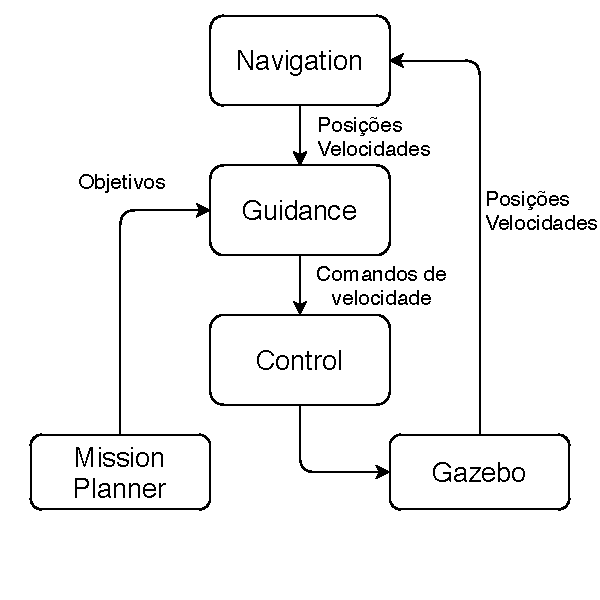
\includegraphics{fig/chap2/arquitetura_base.pdf}
            \caption{Arquitetura do sistema base}
            \label{fig:chap2_arquitetura_base}
        \end{figure}
        
        No sistema GNC desenvolvido por Jurak~\cite{Jurak2020COLREGS}, o entendimento do subsistema \textit{"Guidance"} é o de maior relevância para a compreensão deste trabalho. Como explicado no Capítulo~\ref{subchap2:USV}, o subsistema \textit{"Guidance"} é, em suma, responsável por determinar o caminho a ser seguido pelo USV, gerando comandos de velocidade para o subsistema \textit{"Control"}. O subsistema \textit{"Guidance"} desenvolvido por Jurak~\cite{Jurak2020COLREGS} conta com 2 planejadores, que são algoritmos responsáveis por determinar uma trajetória até uma posição alvo, ambos foram desenvolvidos a partir do pacote ROS chamado \textit{"move\_base"}. Um dos planejadores atua em escopo global (chamado de planejador global), realizando o planejamento da rota (rota global) a partir da posição em que o USV se encontra, até a posição objetivo (objetivo global). A rota global é planejada desviando de obstáculos estáticos (pontes, pedras, ilhas, corais) conhecidos a partir de mapas, cartas náuticas e etc. Já o outro planejador atua em escopo local (chamado de planejador local), sendo responsável pelo comportamento reativo à obstáculos que se aproximam. O planejador local determina o trajeto de curta 
        distância a ser percorrido pelo USV (rota local), desviando da rota global para que seja possível evitar um obstáculo que se aproxima e então retornar para a rota global. A posição alvo do planejador local (objetivo local) é a mais próxima possível da rota global, dentro do mapa local.

       O subsistema de \textit{"Guidance"} também conta com dois mapas de custo, que são representações virtuais do cenário onde o USV se encontra. Um dos mapas representa o cenário como um todo, denominado mapa global, enquanto que o outro mapa representa o entorno do USV, denominado mapa local. Para o caso do sistema de Jurak~\cite{Jurak2020COLREGS}, o mapa local representa uma área de 20mx20m com o USV localizado no centro dele. Os mapas são divididos em linhas e colunas, formando células onde cada uma possui um custo de 0 a 255. Uma célula com custo 0 indica que ela está totalmente livre e o USV consegue passar por ela. Já uma célula com custo 255 indica que a célula está totalmente obstruída e o USV não consegue passar por ela. Com isso, o planejador global e o planejador local podem determinar suas respectivas rotas através das células livres do mapa global e do mapa local. Como o planejador local é responsável pelo comportamento reativo do sistema, ele também é responsável por fazer com que o USV realize um desvio que atenda às requisições das COLREGS. Tais requisições são atendidas através da técnica de custo de terreno artificial (do inglês \textit{"Artificial Terrain Cost"} - ATC), que consiste em criar obstáculos virtuais na região que o USV não pode desviar, dado que essa seria uma região que viola as requisições da COLREGS, fazendo com o planejador local defina uma rota local por uma área que esteja em conformidade com as COLREGS. Esses obstáculos são criados a partir da embarcação que se aproxima até a borda do mapa local. Os obstáculos virtuais consistem em aumentar o custo das células do mapa local em que serão criadas, impossibilitando o planejador local de determinar uma rota que passe pelas células em questão. 
       
       Jurak~\cite{Jurak2020COLREGS} apresenta a Figura~\ref{fig:chap3_sistema_base_costmaps} que ilustra de forma completa os conceitos aqui apresentados. As regiões em tons de cinza indicam o mapa global, onde as células pretas representam obstáculos estáticos que não podem ser transpassados pelo USV. A região azul no entorno do USV (na imagem legendado como \textit{"Own Vessel"}) indica o mapa local, onde as células avermelhadas indicam obstáculos próximos que não podem ser transpassados pelo USV. É possível notar que a outra embarcação (na imagem legendada como \textit{"Encountering Vessel"}) está assinalado como um obstáculo. Também é possível notar a rota global (linha vermelha que parte do USV e vai para além do mapa local) se estendendo até o objetivo global. O objetivo local está indicado na borda do mapa local no ponto mais próximo possível da rota global. A imagem em questão está representando uma localização real, sendo esta o Arroio do Dilúvio na cidade de Porto Alegre no Rio Grande do Sul, Brasil.
       
       \begin{figure}
           \centering
           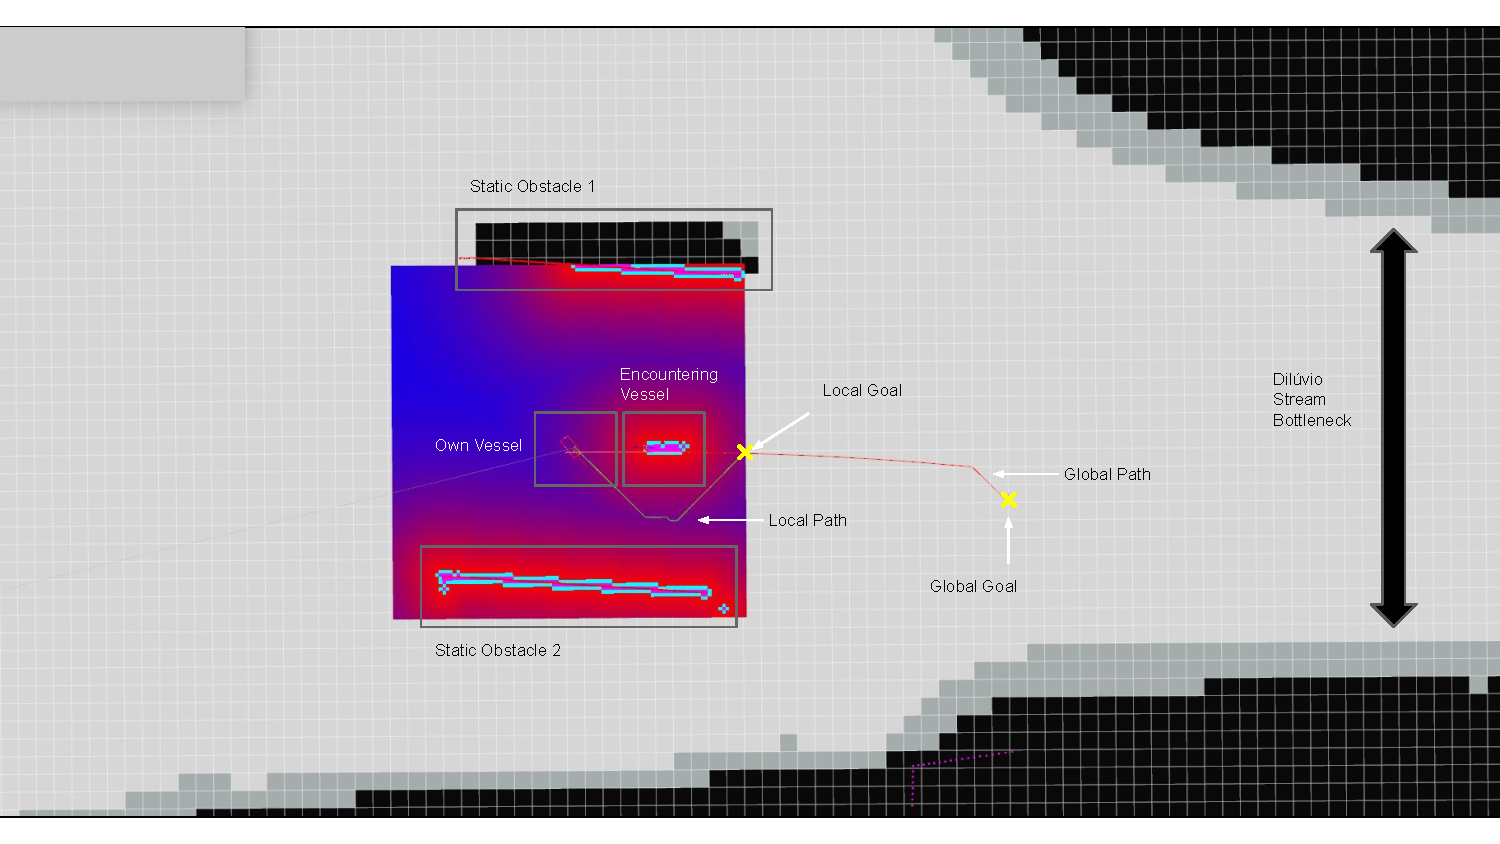
\includegraphics[scale=0.65]{fig/chap3/costmaps.pdf}
           \caption{Imagem apresentada por Jurak~\cite{Jurak2020COLREGS} ilustrando mapa global, mapa local, obstáculos, objetivo global, objetivo local, rota global e rota local}
           \label{fig:chap3_sistema_base_costmaps}
       \end{figure}
%!TEX root = tcc_final.tex
\chapter{Desenvolvimento}\label{chap4:desenvolvimento}

\frm[inline]{Digamos que isto está um pouco, curto. }
    % - Falar sobre as informações necessárias para o desenvolvimento
    % - Falar sobre o local onde o CPA foi integrado (em detalhes)
    % - Falar sobre o desenvolvimento em si
    %   - Colocar fórmulas dos vetores
    %   - Explicar profundamente as equações
    % - Falar sobre o que foi feito para a coleta dos resultados
    %   - Criação dos tópicos para publicar t_cpa e d_cpa
    
    O desenvolvimento deste trabalho resume-se à implementação da Equação~\ref{eq:tcpa} e da Equação~\ref{eq:dcpa}.\frm{Se eu bem me recordo, tu tiveste que mexer em bem mais coisas para fazer tudo rodar, não? Eu diria que esta frase vende teu trabalho barato... Tenta explicar que tu tiveste que tunar parâmetros também...} 
    Obtendo os valores resultantes, aplica-se a Desigualdade~\ref{eq:cpaThreshold} para determinar se há risco de colisão ou não. Para tal, usou-se informações referente à posições e velocidades das embarcações que já estavam disponíveis no sistema base. Além disso foi preciso identificar onde, no sistema desenvolvido por Jurak~\cite{Jurak2020COLREGS}, a implementação do ponto de maior proximidade (do inglês \textit{"Closest Point of Approach"} - CPA) seria realizada, para que implementação e integração ocorressem paralelamente. 
    Como citado no Capítulo~\ref{subchap3:sistema_base}, o sistema base cria obstáculos artificiais para fazer com que seu planejador local encontre uma rota que seja compatível com as COLREGS. 
    Logo, identificamos que os obstáculos virtuais deveriam ser criados somente quando houver risco de colisão, caso contrário os obstáculos virtuais não devem ser criados. 
    A Figura~\ref{fig:chap4_fluxograma_inicial} apresenta o fluxograma da rotina onde os obstáculos virtuais são criados antes da implementação do CPA. 
    Com base no fluxograma apresentado, chegamos a conclusão que a implementação do CPA deveria ser realizada no momento anterior à criação dos obstáculos virtuais. 
    A Figura~\ref{fig:chap4_fluxograma_final} apresenta o fluxograma da rotina onde os obstáculos virtuais são criados após a implementação do CPA. 
    Para fins de análise, foi adicionado no sistema base dois tópicos para a publicação do \tcpa e do \dcpa encontrados. Essas informações foram coletadas dos tópicos criados durante as execuções dos testes e gravadas em um arquivo \textit{".bag"}. As informações coletadas serão apresentadas no Capítulo~\ref{chap5:resultados}.
    
    \begin{figure}
        \centering
        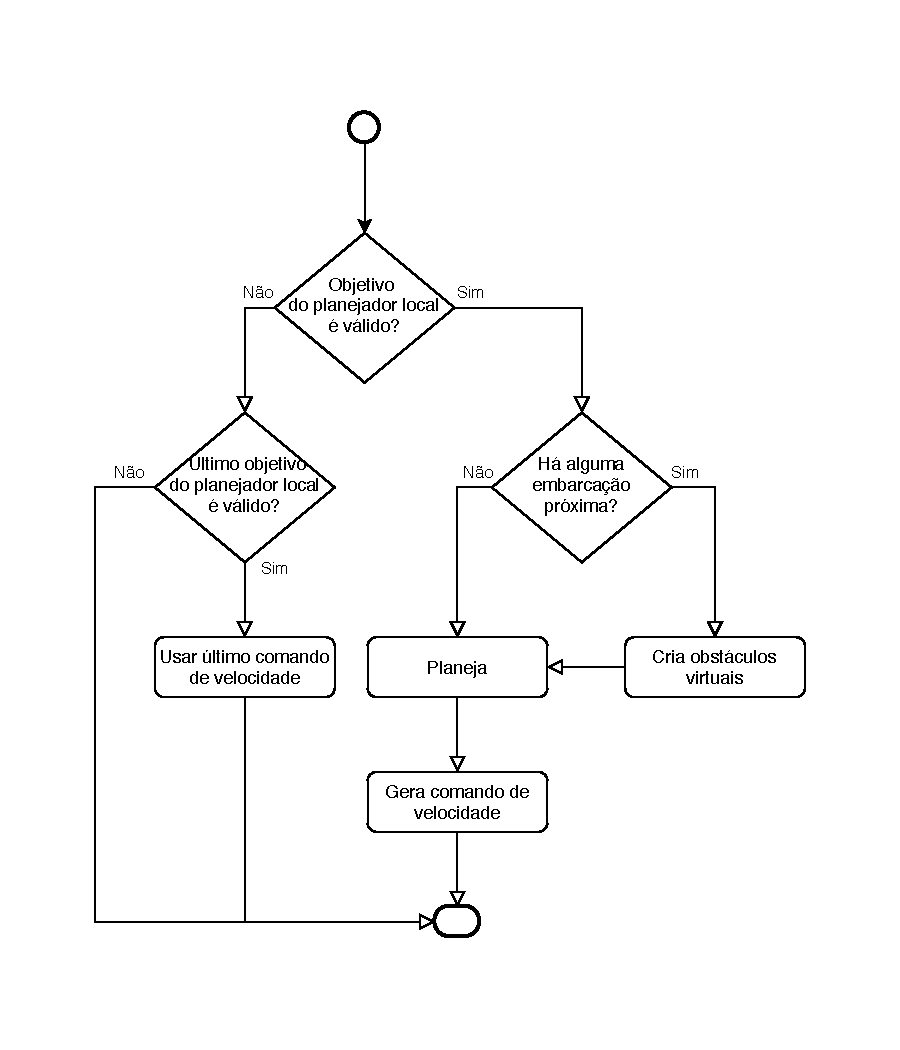
\includegraphics{fig/chap4/find_best_path_diagram_no_cpa.pdf}
        \caption{Fluxograma inicial da rotina onde o CPA foi adicionado.}
        \label{fig:chap4_fluxograma_inicial}
    \end{figure}
    
    \begin{figure}
        \centering
        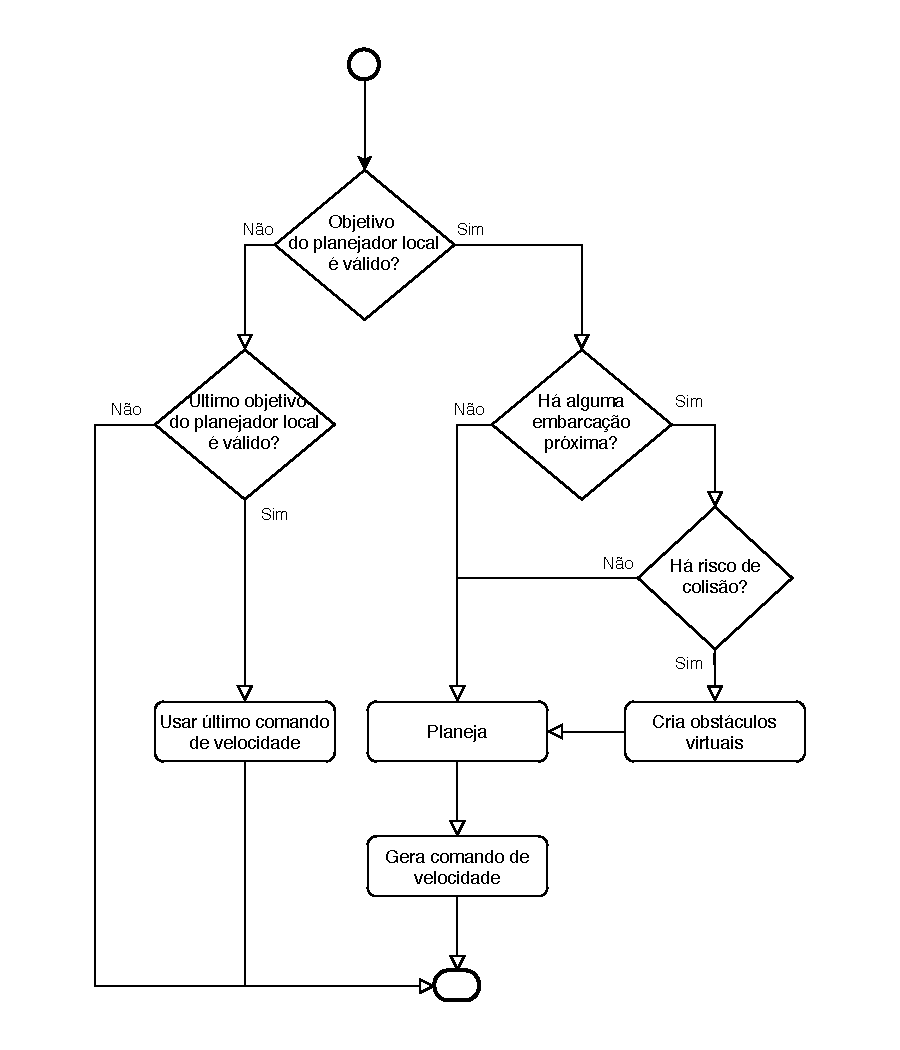
\includegraphics{fig/chap4/find_best_path_diagram_cpa.pdf}
        \caption{Fluxograma final da rotina onde o CPA foi adicionado.}
        \label{fig:chap4_fluxograma_final}
    \end{figure}
    
    % --------------------------------------
    % -------------- QUESTÕES --------------
    % --------------------------------------
    
    % 1) Explicação do CPA deveria estar, na verdade, no capítulo de fundamentação teórica
    % 2) Penso em colocar código no documento final, sinto que não há muito o que falar da implementação, apenas que implementamos os cálculos.
%!TEX root = tcc_final.tex
\chapter{Resultados}\label{chap5:resultados}
    Neste capítulo apresentaremos os testes executados para validar a implementação realizada neste trabalho. Para que seja possível termos um bom comparativo, realizamos os mesmos testes feitos por Jurak~\cite{Jurak2020COLREGS} em seu trabalho. Logo, testamos as alterações realizadas no sistema base para os encontros \textit{"Head On"}, \textit{"Overtaking"}, \textit{"Crossing from Left"} e \textit{"Crossing from Right"}. Com o intuito de evidenciar nossa implementação, realizamos um caso de teste adicional de \textit{"Crossing from Right"} onde a outra embarcação encontra-se parada e afastada o suficiente para que, quando executado com CPA, o sistema não considere uma situação de risco. Mesmo estando mais afastada, em um dado momento a outra embarcação é detectada pelo planejador local, fazendo com que ela seja considerada nas rotas locais planejadas a partir de então. Realizamos esse último caso de teste com e sem CPA. Para fins de análise apresentaremos as trajetórias realizadas pelas embarcações durante o teste, a distância entre elas, o tempo computacional necessário para planejar a rota local e \tcpa e o \dcpa calculados.
    
    Os testes foram realizados utilizando a ferramenta de simulação USV\_sim\footnote{\url{https://github.com/disaster-robotics-proalertas/usv_sim_lsa}}~\cite{Paravisi2018Toward}. Nela, utilizamos o barco de propulsão mostrado na Figura~\ref{fig:chap5_boat}. Os testes foram executados em um cenário virtual que simula o Arroio do Dilúvio, localizado em Porto Alegre - RS. Este cenário foi o mesmo utilizado por Jurak~\cite{Jurak2020COLREGS} em seu trabalho, que também apresenta a Figura~\ref{fig:chap5_diluvio}, ilustrando ambiente real (Figura~\ref{fig:chap5_diluvio_real}) e o ambiente simulado (Figura~\ref{fig:chap5_diluvio_simulado}).
    
    \begin{figure}[H]
		\centering
        \begin{subfigure}{0.4\textwidth}
            \centering
            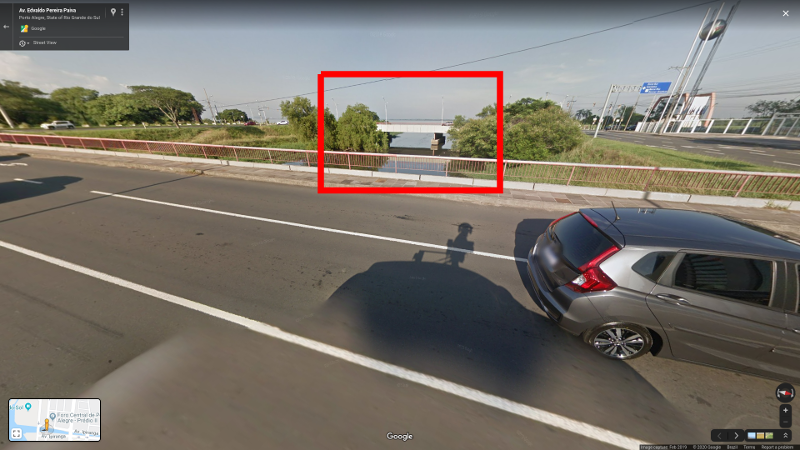
\includegraphics[width=\textwidth]{fig/chap5/diluvio_real.png}
            \caption{}
            \label{fig:chap5_diluvio_real}
        \end{subfigure}
        \begin{subfigure}{0.4\textwidth}
            \centering
            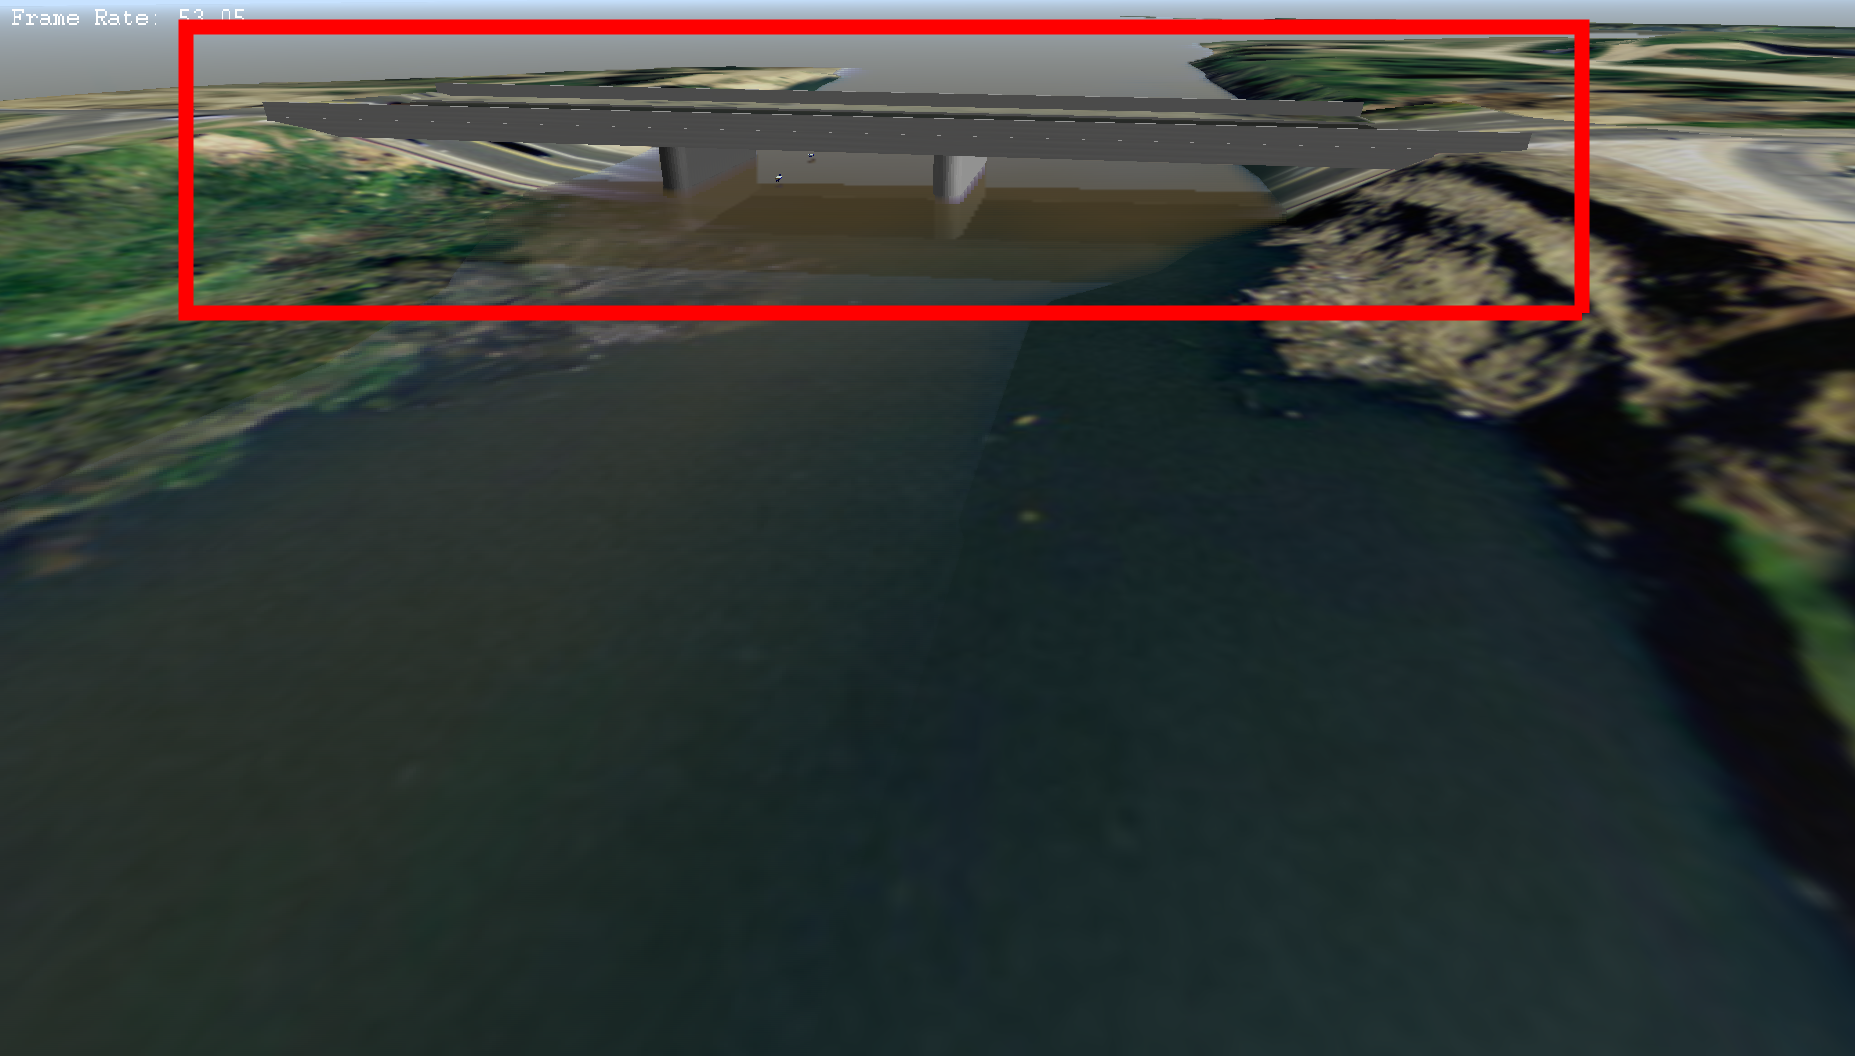
\includegraphics[width=\textwidth]{fig/chap5/diluvio_simulado.png}
            \caption{}
            \label{fig:chap5_diluvio_simulado}
        \end{subfigure}
    
    \caption{Ambiente real e ambiente simulado, apresentado por Jurak~\cite{Jurak2020COLREGS}}
    \label{fig:chap5_diluvio}
    \end{figure}
    % Comentário para evitar novo parágrafo
    \begin{figure}[H]
        \centering
        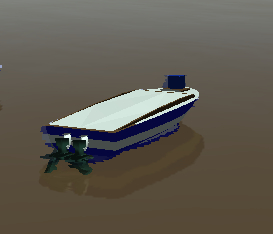
\includegraphics[scale=0.5]{fig/chap5/boat.jpg}
        \caption{Barco de propulsão utilizado nos testes.}
        \label{fig:chap5_boat}
    \end{figure}
    
    \section{Head On} \label{subchap5_headon}
        
        A Figura~\ref{fig:chap5_headon_paths} mostra a trajetória realizada pelas embarcações para o caso de teste \textit{"Head On"}, onde as embarcações vão uma de encontro a outra frente a frente. A linha azul representa o trajeto realizado pelo USV enquanto que a linha vermelha representa o trajeto realizado pela outra embarcação. Os pequenos triângulos, em cada uma das trajetórias no gráfico, indicam o sentido em que as embarcações se deslocaram e a posição em que cada uma das embarcações estava quando a distância entre elas foi a menor registrada durante todo o teste. A 
        distância, nesse caso, foi de 2,419m. A Figura~\ref{fig:chap5_headon_cpa} mostra as informações coletadas durante o teste a respeito do CPA. A Figura~\ref{fig:chap5_headon_tcpa} mostra graficamente, no tempo, o \tcpa calculado. O eixo horizontal representa unidades de tempo e o eixo vertical representa o \tcpa calculado na unidade de segundos, essas informações são válidas para todos os gráficos de \tcpa apresentados daqui para frente. Os vales gerados no gráficos indicam que a condição $\Vert\vec{v}_{A}-\vec{v}_{B}\Vert < \epsilon$ foi satisfeita e o \tcpa foi considerado zero. Nos momentos em que a 
        condição $\Vert\vec{v}_{A}-\vec{v}_{B}\Vert < \epsilon$ não é satisfeita, é possível observar inicialmente um decremento do \tcpa calculado e então um aumento. Isso indica uma aproximação das embarcações e logo após um distanciamento das mesmas.
        Já a Figura~\ref{fig:chap5_headon_dcpa} mostra graficamente, no tempo, o \dcpa calculado. O eixo horizontal representa unidades de tempo e o eixo vertical representa o \dcpa calculado na unidade de metros, essas informações são válidas para todos os gráficos de \dcpa apresentados daqui para frente. Nessa imagem, é possível observar o impacto que a condição $\Vert\vec{v}_{A}-\vec{v}_{B}\Vert < \epsilon$ ser satisfeita gera no resultado do \dcpa, também resultando em vales no gráfico. A Figura~\ref{fig:chap5_headon_computation_time} mostra o tempo de computação necessário para a execução da rotina apresentada no 
        Capítulo~\ref{chap4:desenvolvimento}. O eixo horizontal representa unidades de tempo e o eixo vertical representa o tempo (em milissegundos) consumido para a execução da rotina, essas informações são válidas para todos os gráficos de esforço computacional apresentados daqui para frente. O gráfico indica que o teste começa com os maiores tempos de computação dado que a distância inicial entre as embarcações é pequena o suficiente para ser considerada situação de risco, sendo necessária a criação dos obstáculos virtuais.
        
        \frm[inline]{Aumenta a fonte das figuras e tenta colocar elas lado a lado, para agrupar figuras do mesmo experimentom senão fica complicado de ver elas.}
        
        \begin{figure}[H]
            \centering
            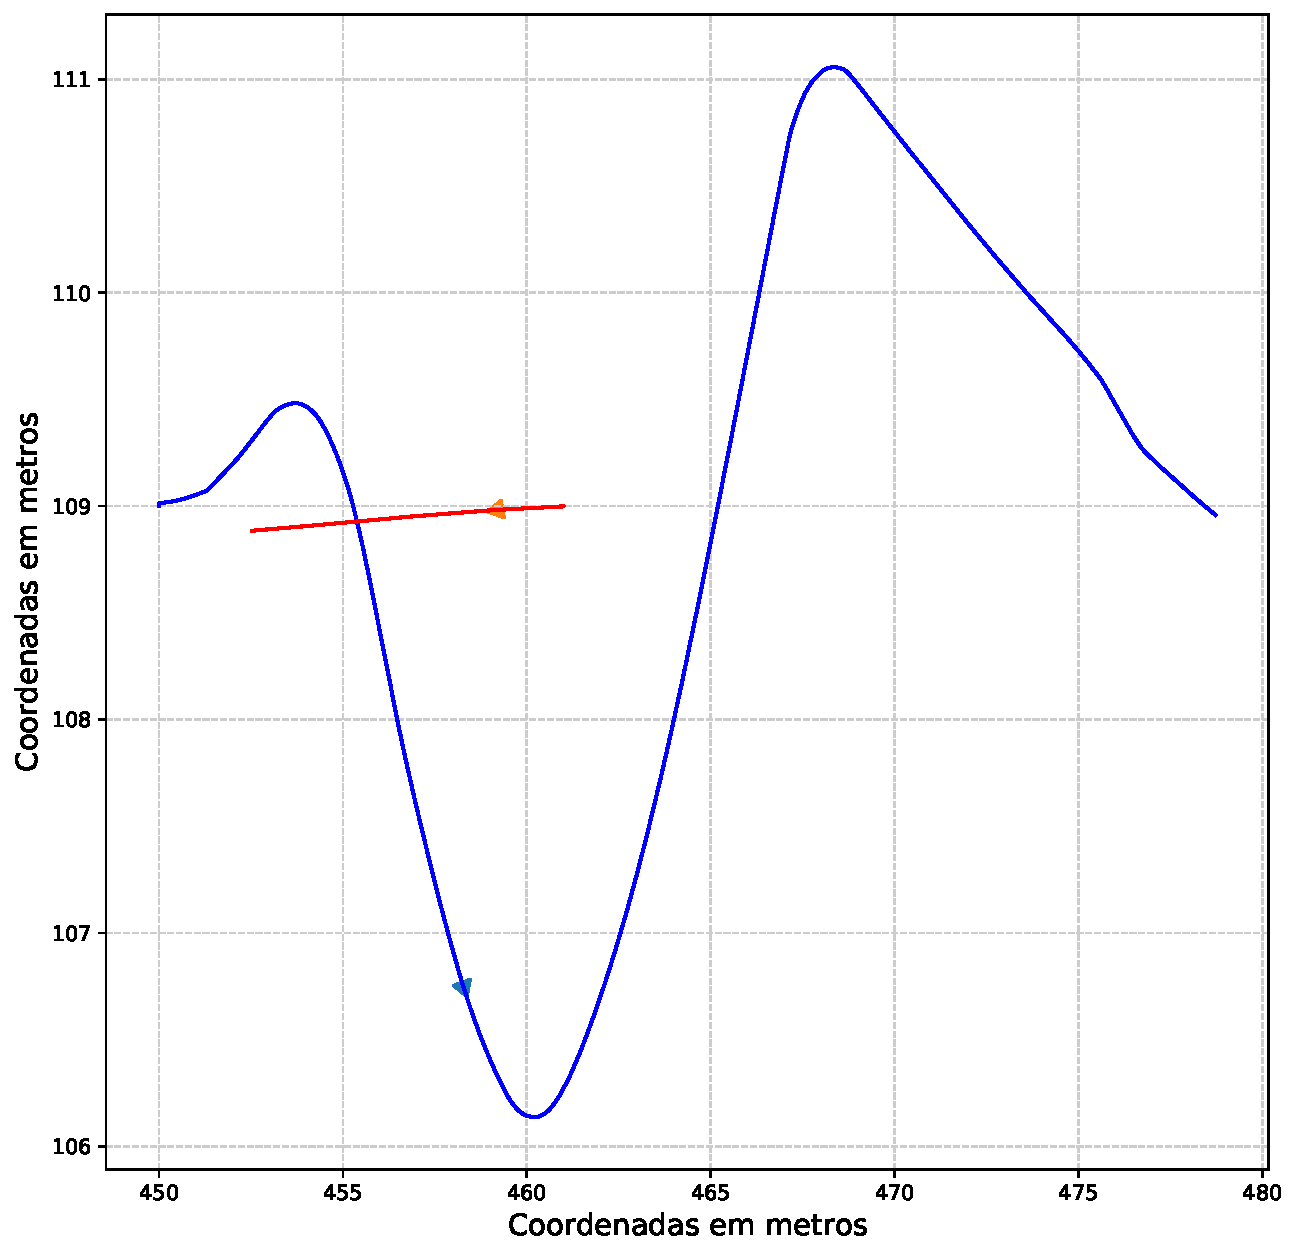
\includegraphics[scale=0.45]{fig/chap5/headon_cpa_trajectory.pdf}
            \caption{Trajeto das embarcações}
            \label{fig:chap5_headon_paths}
        \end{figure}
        
        \begin{figure}[H]
		\centering
% 		\begin{subfigure}{0.5\textwidth}
		\begin{subfigure}{1\textwidth}
            \centering
            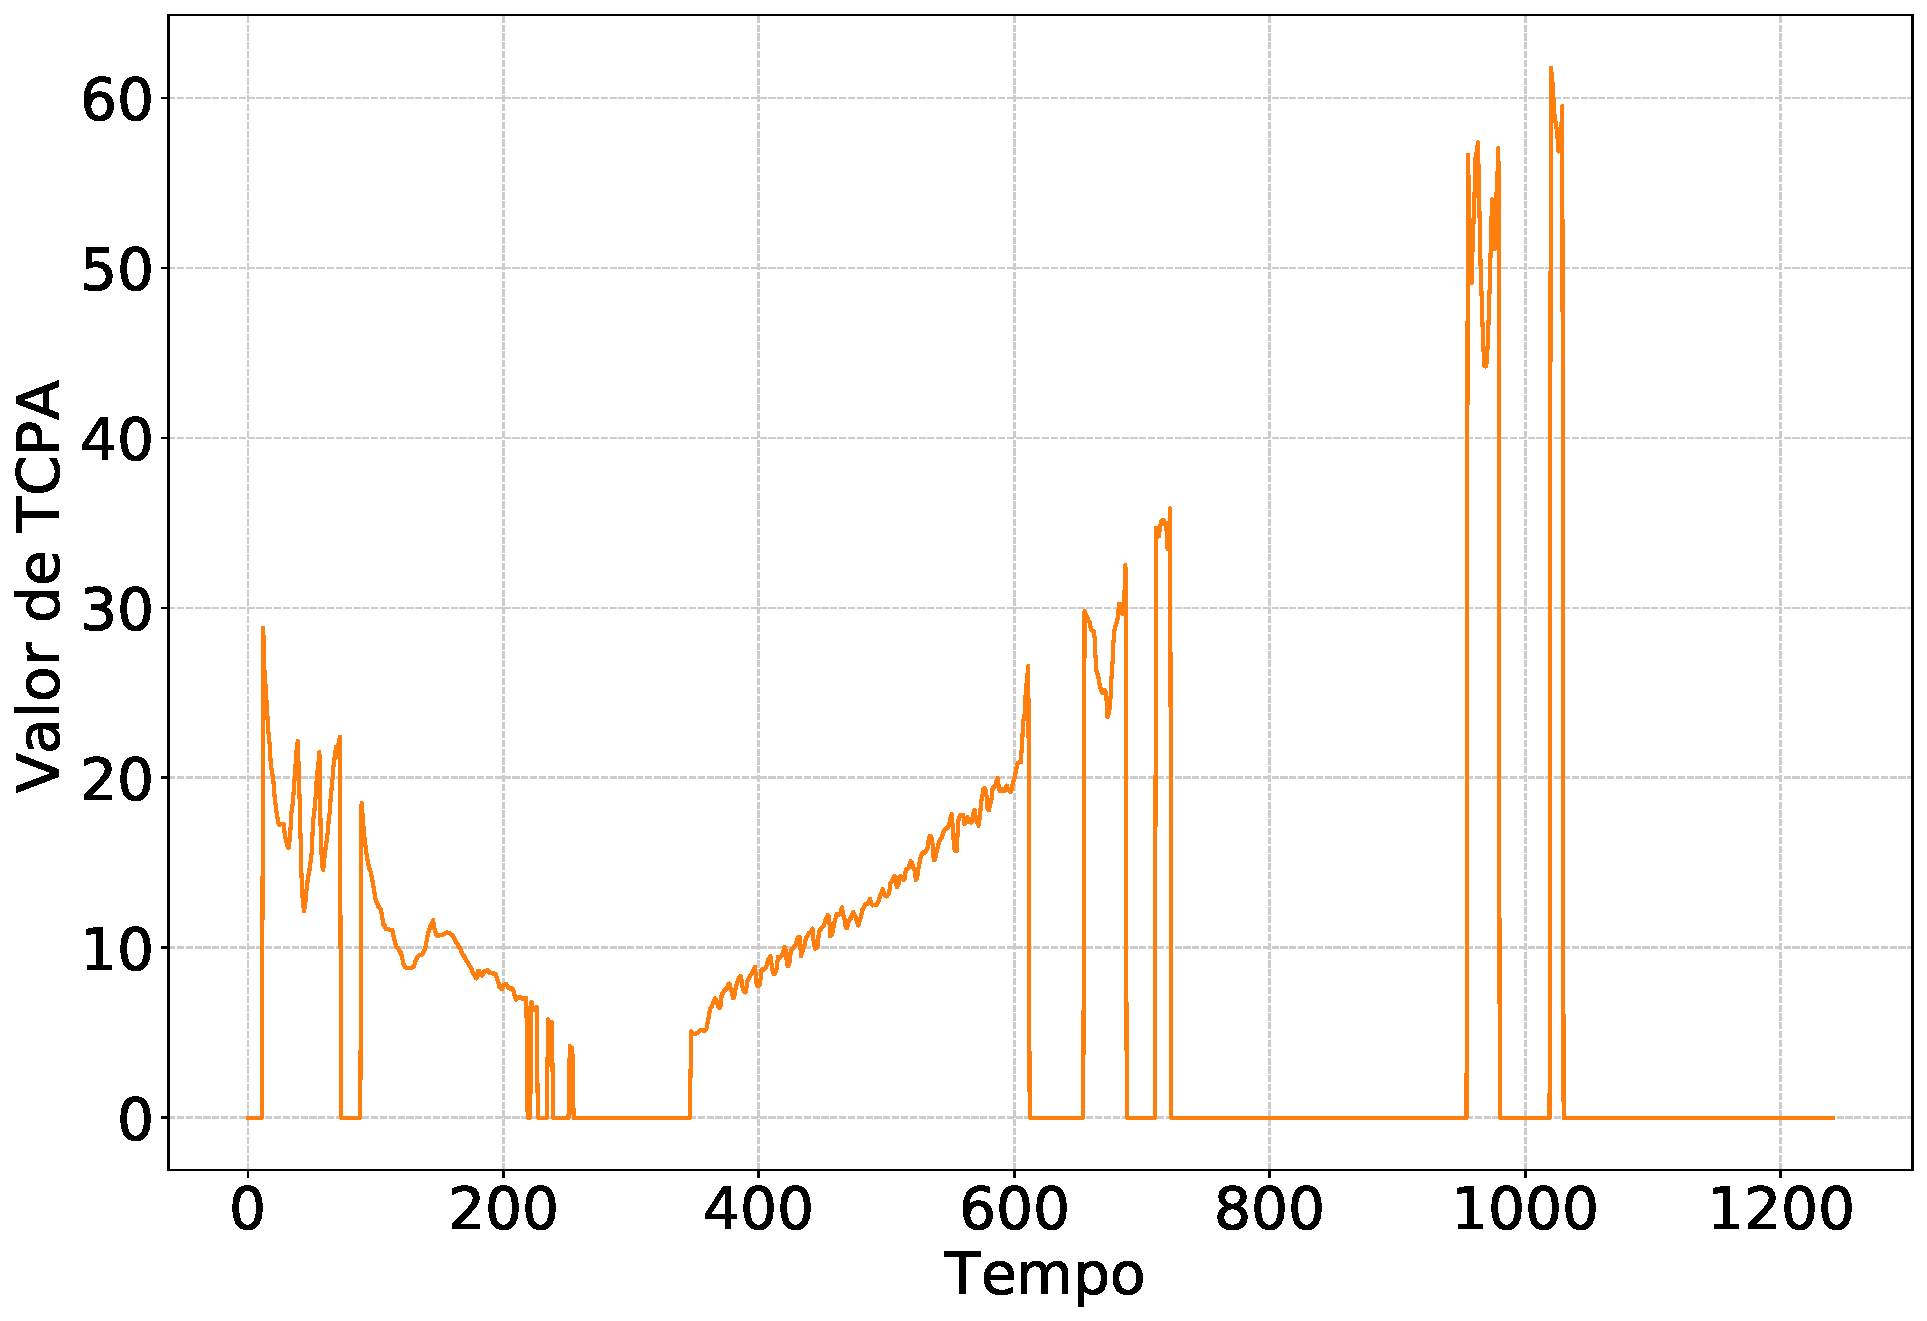
\includegraphics[width=\textwidth]{fig/chap5/headon_tcpa.pdf}
            \caption{TCPA}
            \label{fig:chap5_headon_tcpa}
        \end{subfigure}
% 		\begin{subfigure}{0.5\textwidth}
        \begin{subfigure}{1\textwidth}
            \centering
            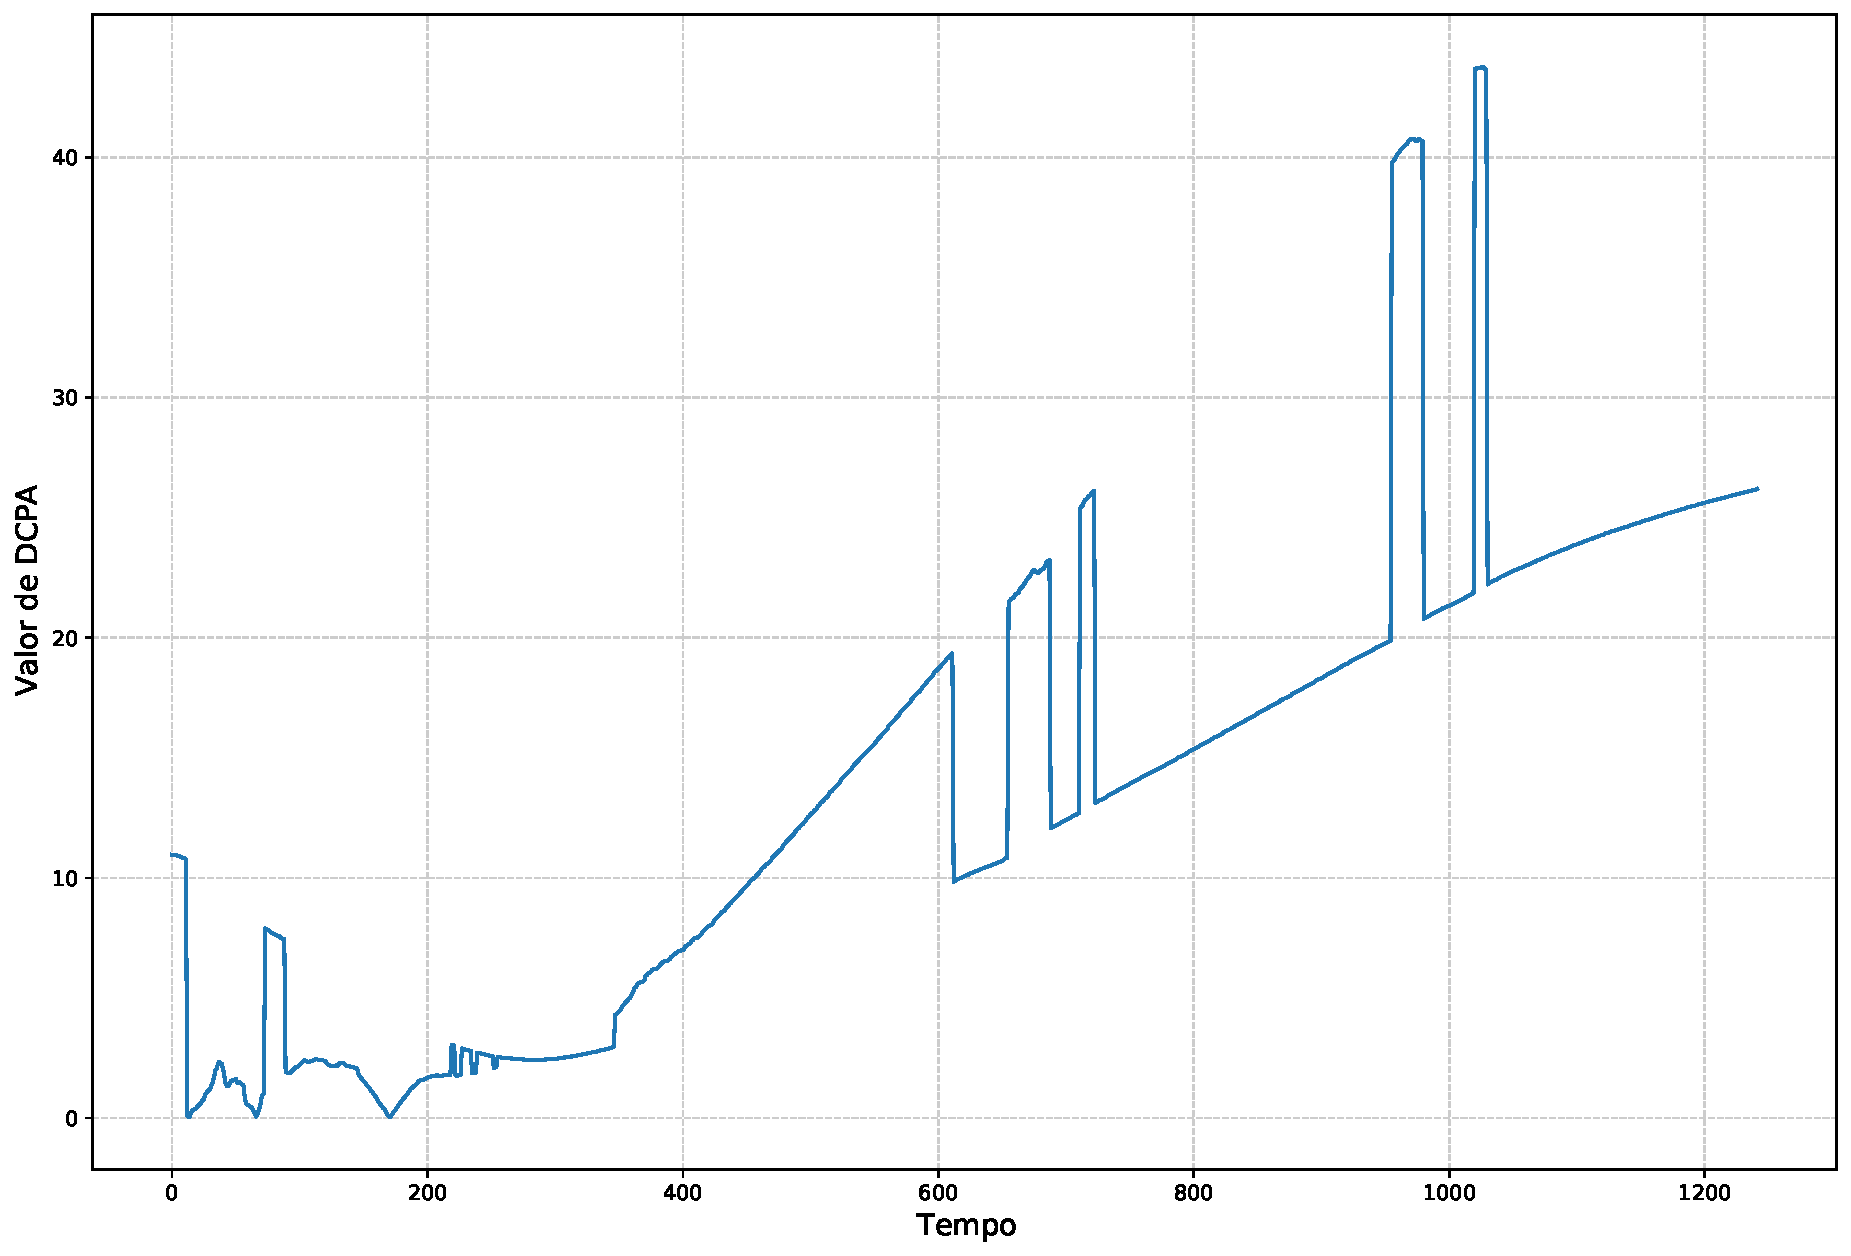
\includegraphics[width=\textwidth]{fig/chap5/headon_dcpa.pdf}
            \caption{DCPA}
            \label{fig:chap5_headon_dcpa}
        \end{subfigure}
        
        \caption{Informações do CPA}
        \label{fig:chap5_headon_cpa}
        \end{figure}
        
        \begin{figure}[H]
            \centering
            % 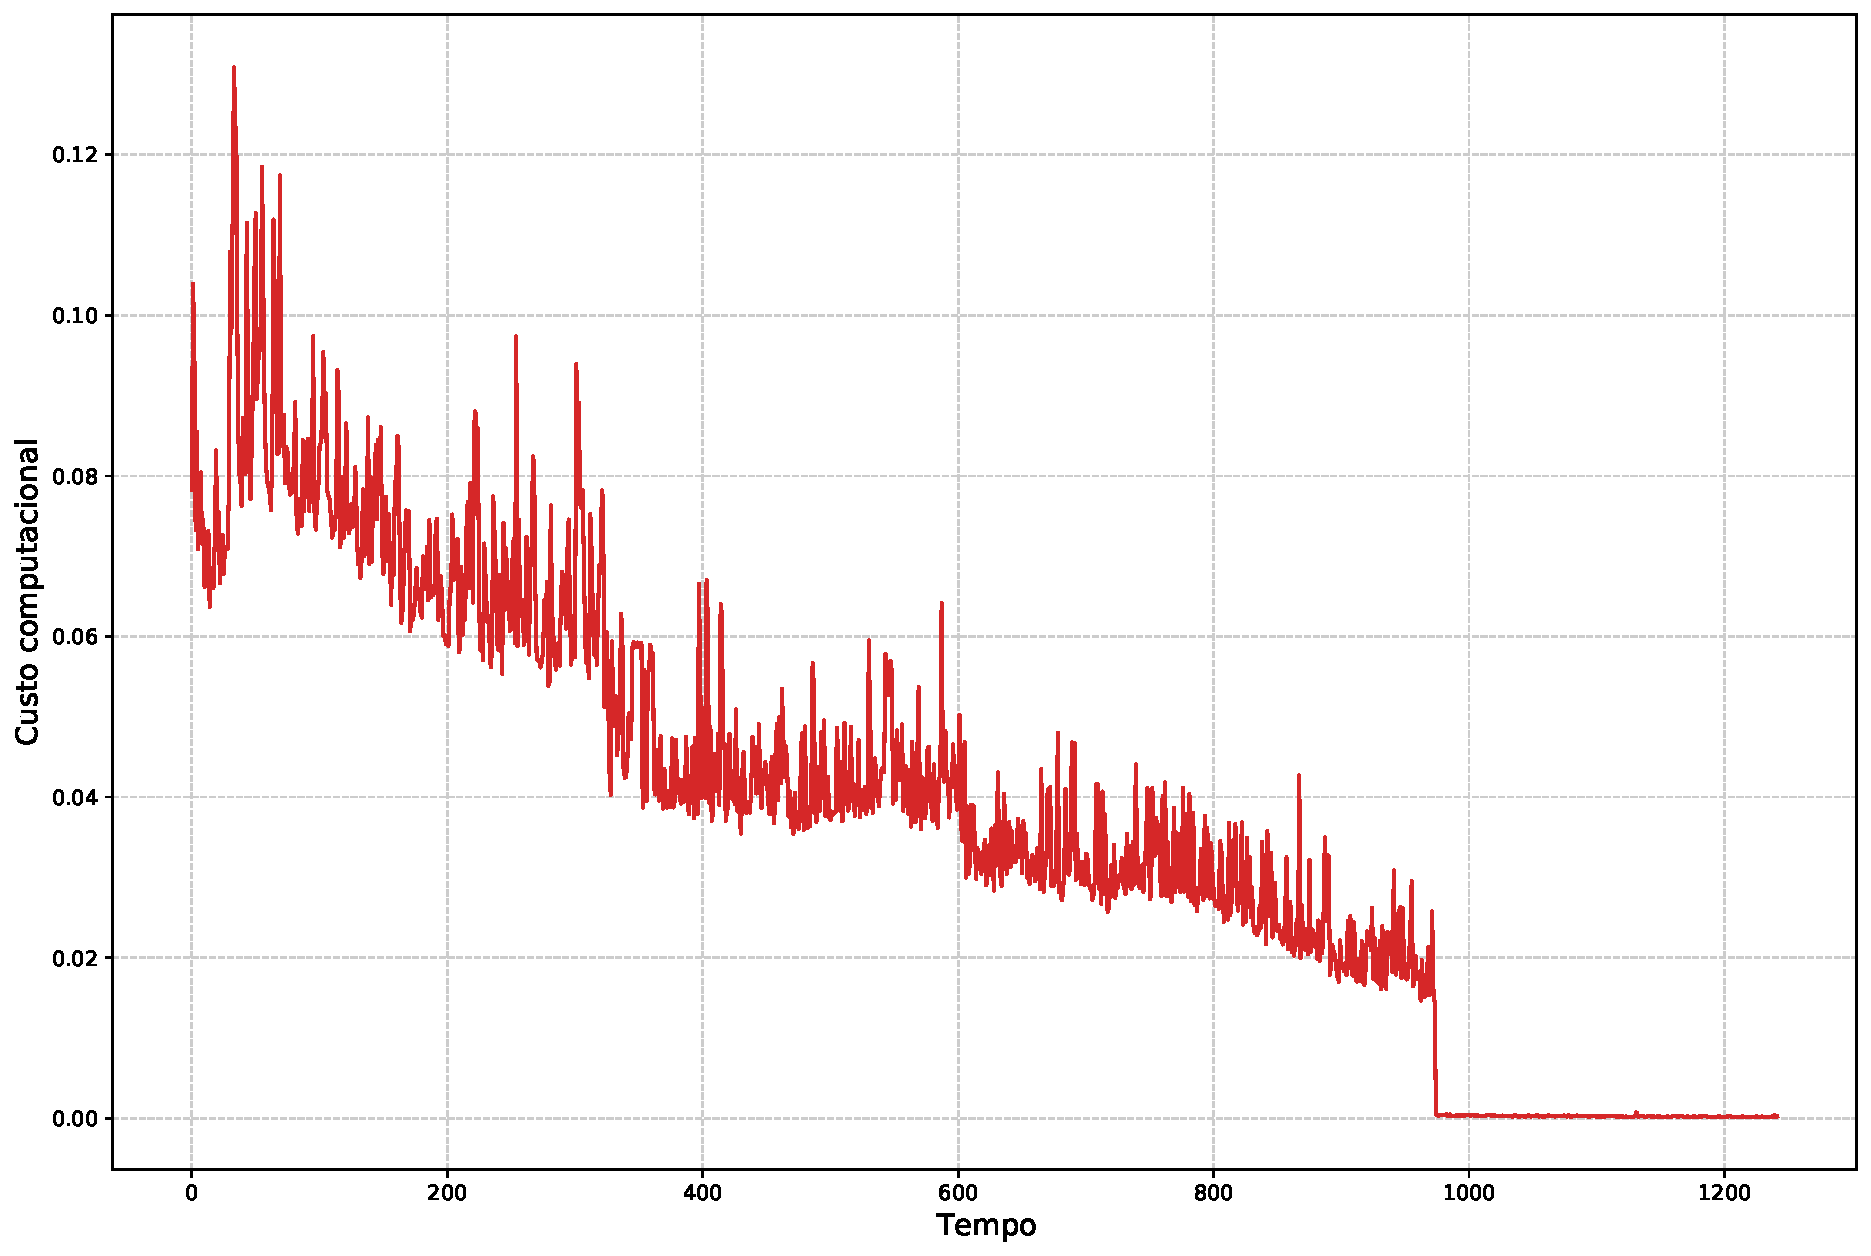
\includegraphics[width=0.3\textwidth]{fig/chap5/headon_computation_time.pdf}
            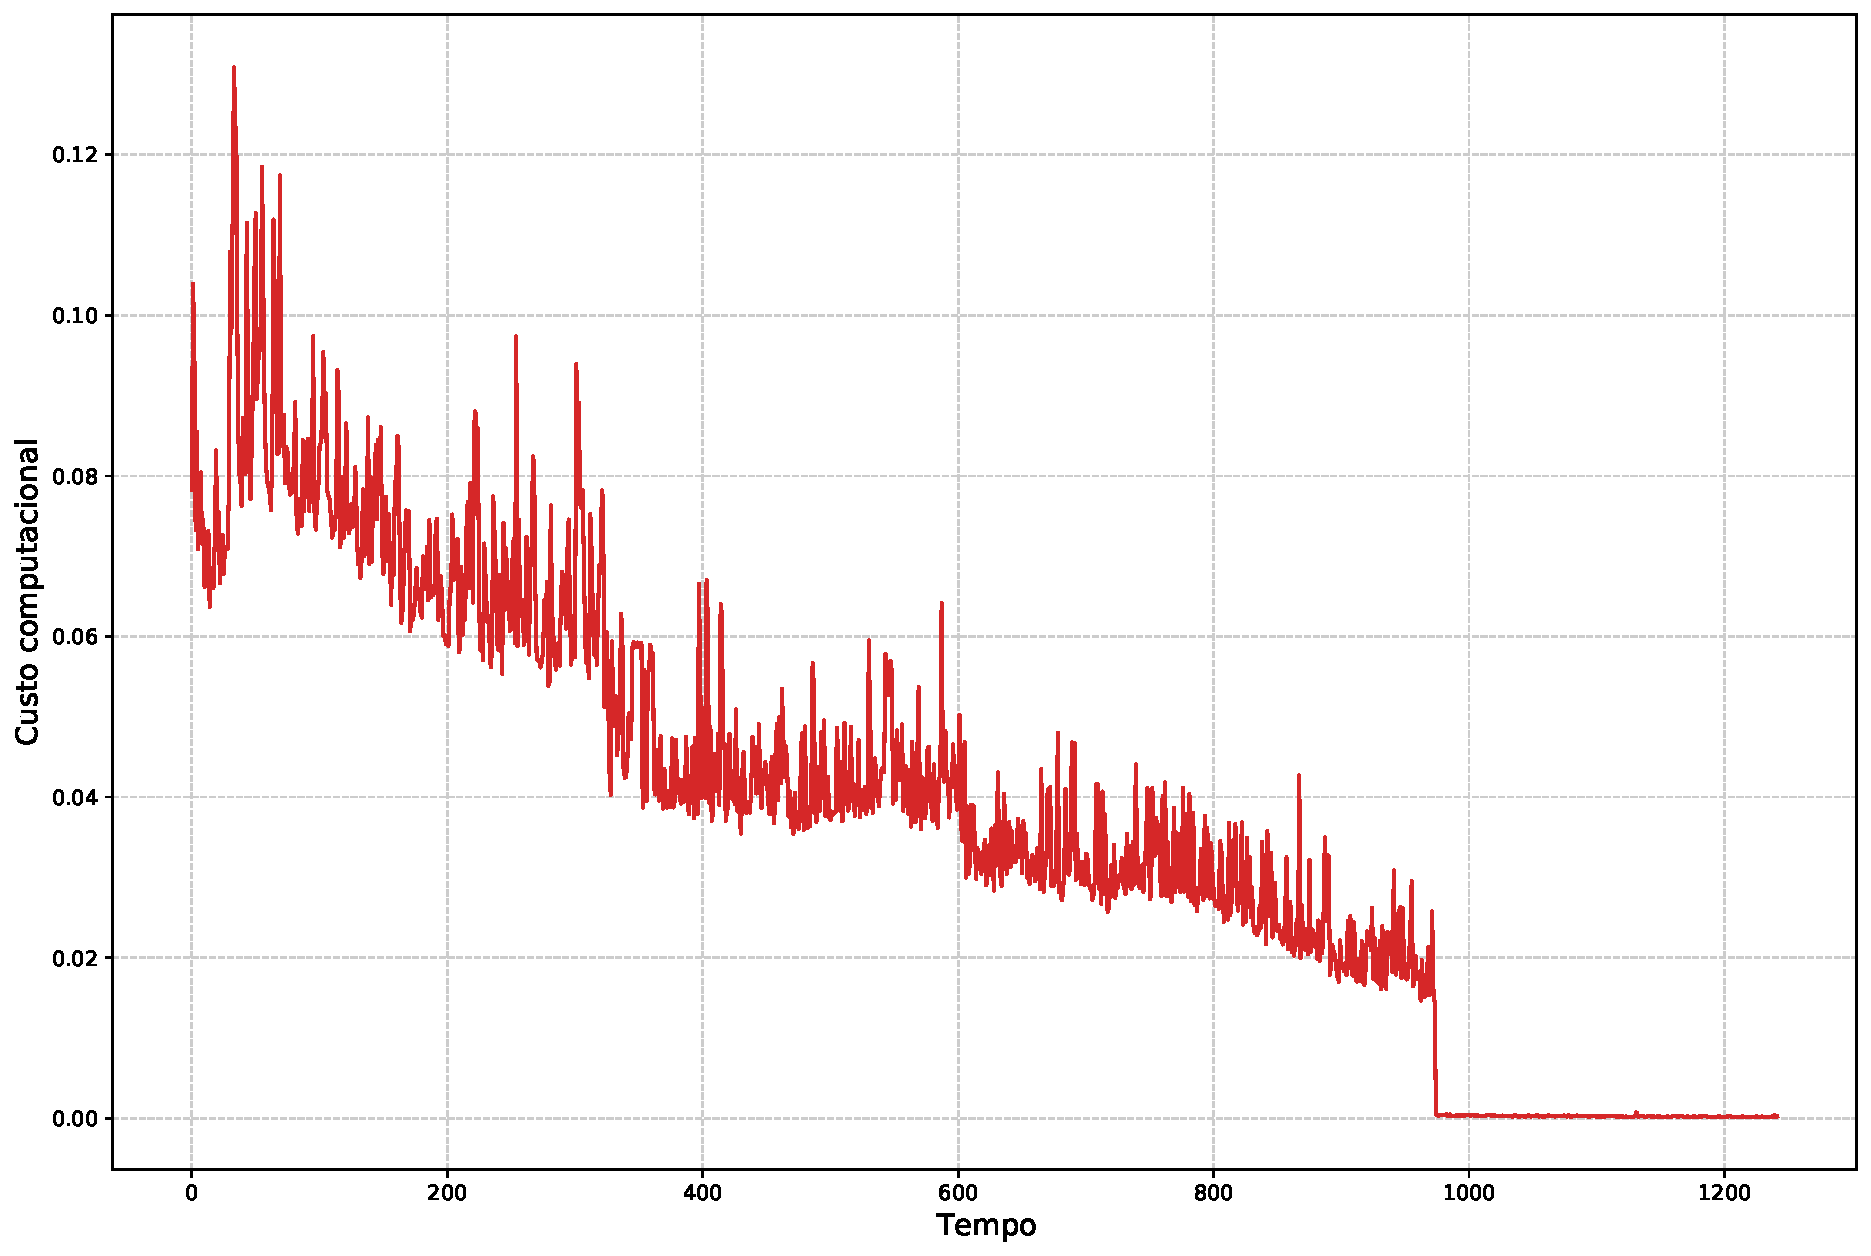
\includegraphics[width=\textwidth]{fig/chap5/headon_computation_time.pdf}
            \caption{Tempo de computação}
            \label{fig:chap5_headon_computation_time}
        \end{figure}
        
    \section{Overtake} \label{subchap5_overtake}
        A Figura~\ref{fig:chap5_overtake_paths} mostra o trajeto resultante para o caso de teste \textit{"Overtake"}. Nesse caso, as embarcações se deslocam na mesma direção e o USV realiza a manobra para ultrapassar a outra embarcação. A linha azul representa o trajeto realizado pelo USV enquanto que a linha vermelha representa o trajeto realizado pela outra embarcação. Os pequenos triângulos, em cada uma das trajetórias no gráfico, indicam o sentido em que as embarcações se deslocaram e a posição em que cada embarcação estava no momento em que foi registrada a menor distância entre elas durante todo o teste. Nesse caso, a distância foi de 2,255m. A Figura~\ref{fig:chap5_overtake_cpa} mostra as informações do CPA coletadas durante o teste. A análise da Figura~\ref{fig:chap5_overtake_tcpa} e da Figura~\ref{fig:chap5_overtake_dcpa} são análogas às análises realizadas na Seção~\ref{subchap5_headon}. Entretanto, é possível observar no início do gráfico, mostrado na Figura~\ref{fig:chap5_overtake_dcpa}, que houve um pico da estimativa de 
        distância, ocasionado pela decisão do USV de primeiro fazer uma curva para esquerda para só então executar o \textit{"Overtake"} pela direita da outra embarcação. A primeira conversão à esquerda é realizada pelo USV dado que, no início do teste, há um obstáculo estático à sua direita. Sua decisão em realizar o \textit{"Overtake"} pela direita se justifica pela COLREGS, que afirma que essa manobra deve ser realizada de forma que não configure novamente uma situação de \textit{"Overtake"}. A análise da Figura~\ref{fig:chap5_overtake_computation_time} é análoga à análise realizada anteriormente no Capítulo~\ref{subchap5_overtake}.
       
    
        \begin{figure}[H]
            \centering
            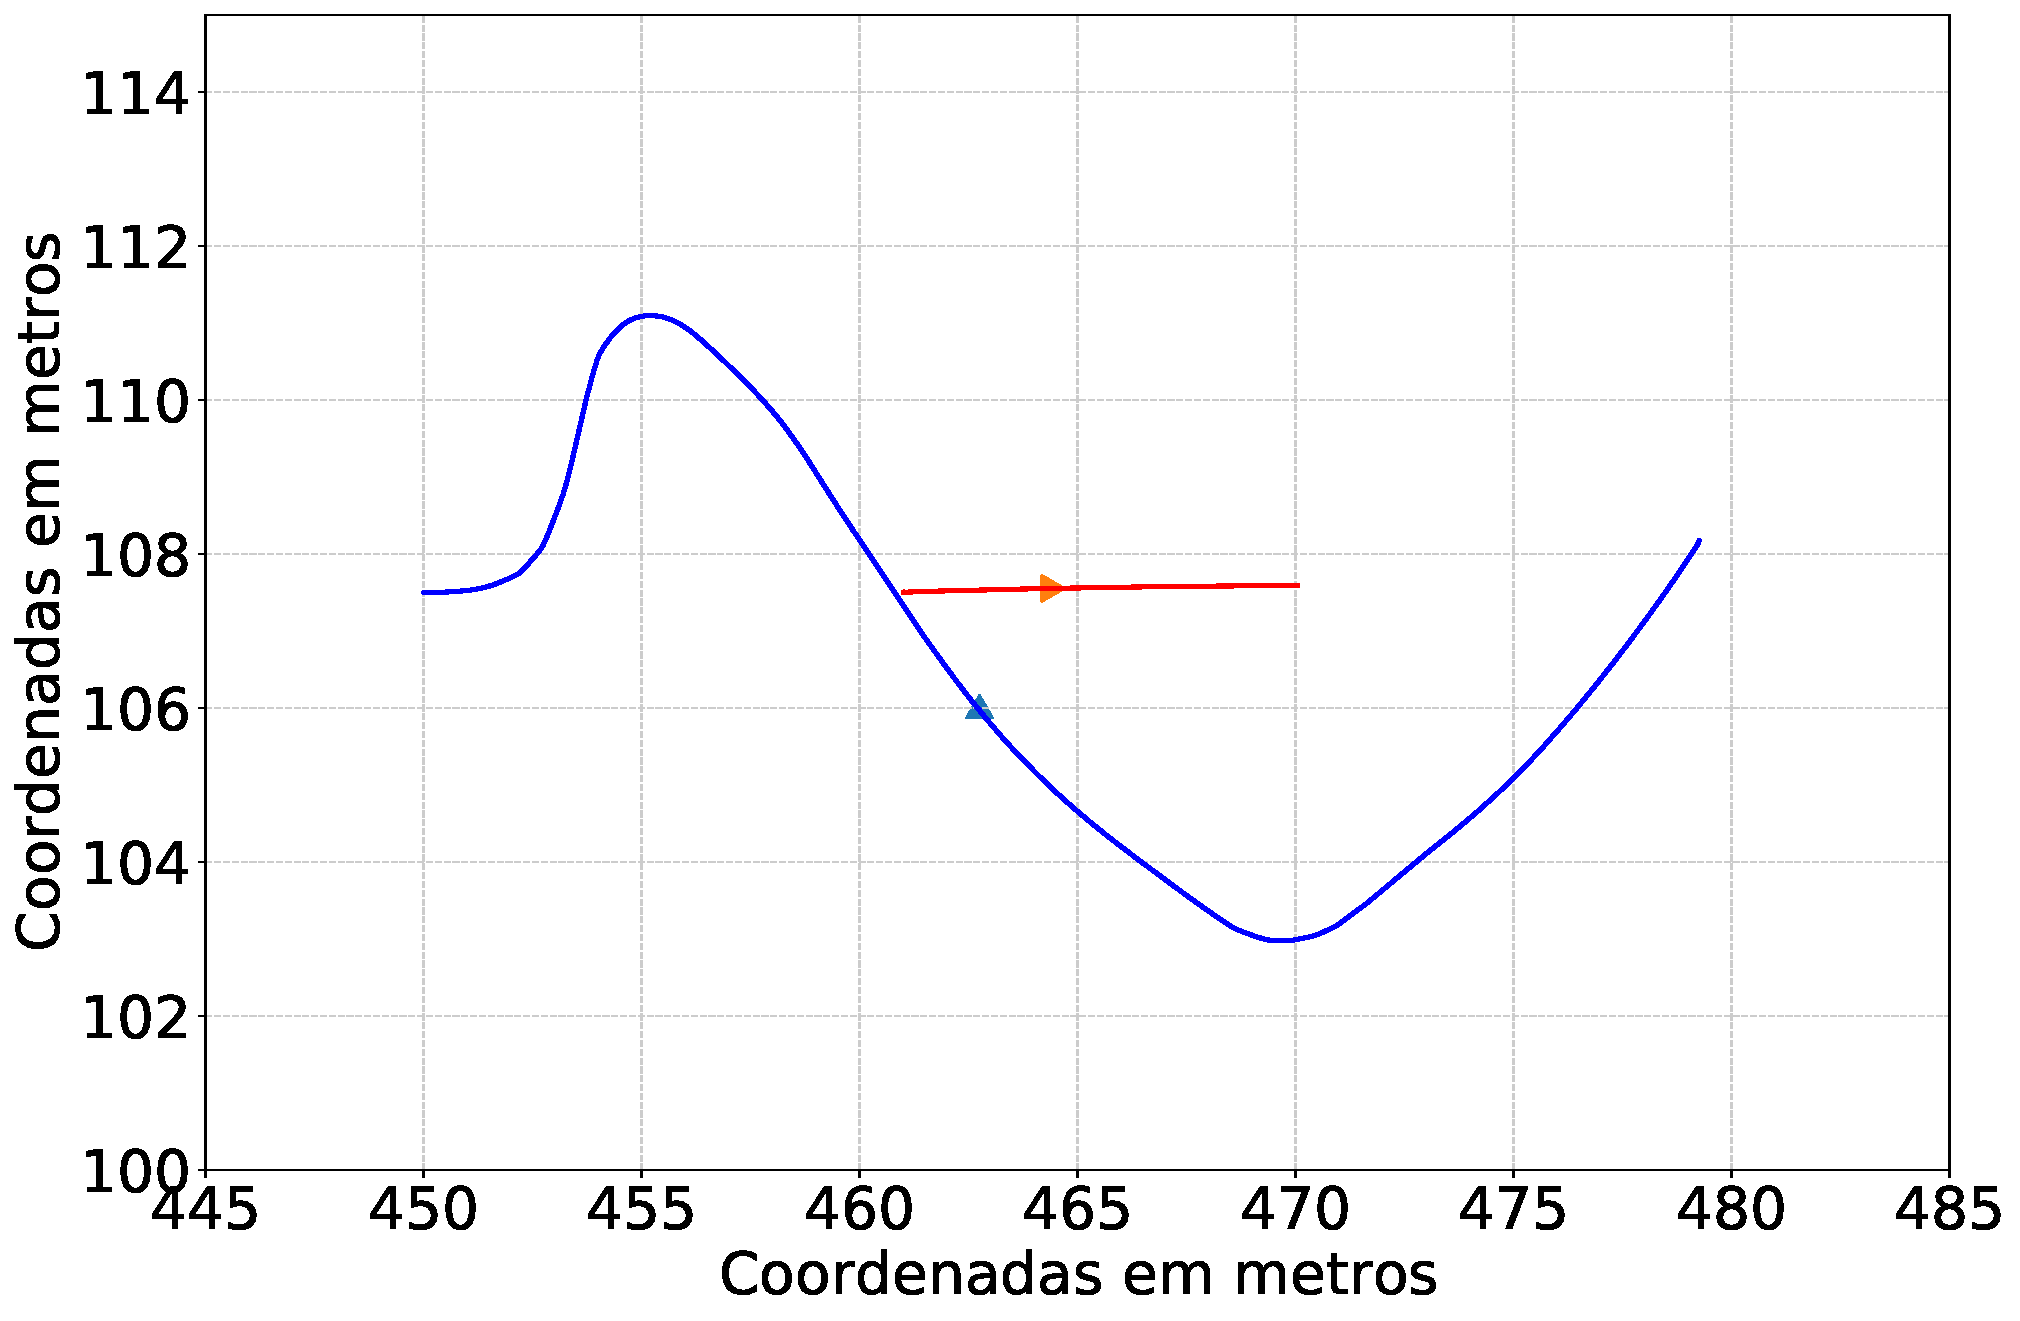
\includegraphics[scale=0.45]{fig/chap5/overtake_trajectory.pdf}
            \caption{Trajeto das embarcações}
            \label{fig:chap5_overtake_paths}
        \end{figure}
        
        \begin{figure}[H]
		\centering
% 		\begin{subfigure}{0.5\textwidth}
		\begin{subfigure}{1\textwidth}
            \centering
            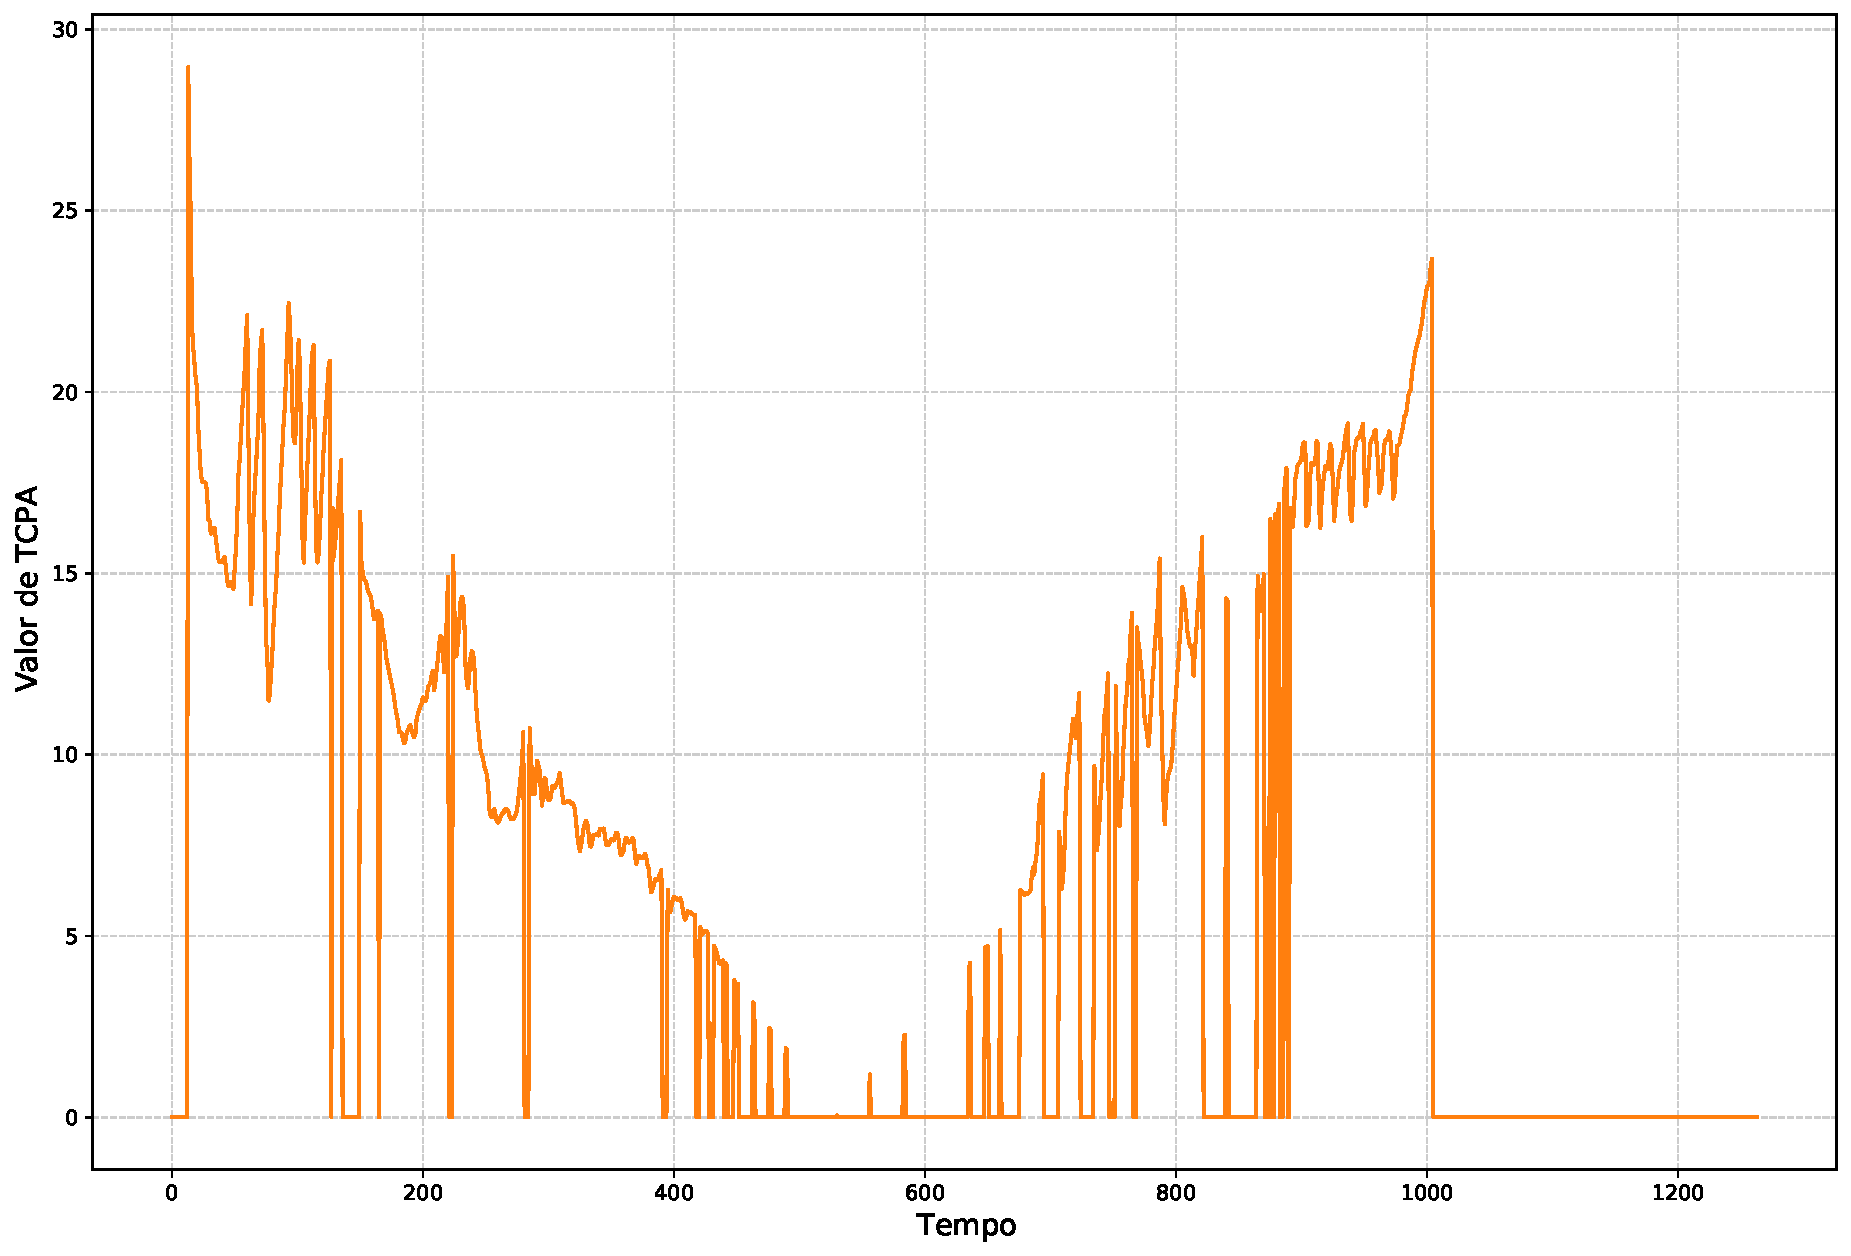
\includegraphics[width=\textwidth]{fig/chap5/overtake_tcpa.pdf}
            \caption{TCPA}
            \label{fig:chap5_overtake_tcpa}
        \end{subfigure}
% 		\begin{subfigure}{0.5\textwidth}
        \begin{subfigure}{1\textwidth}
            \centering
            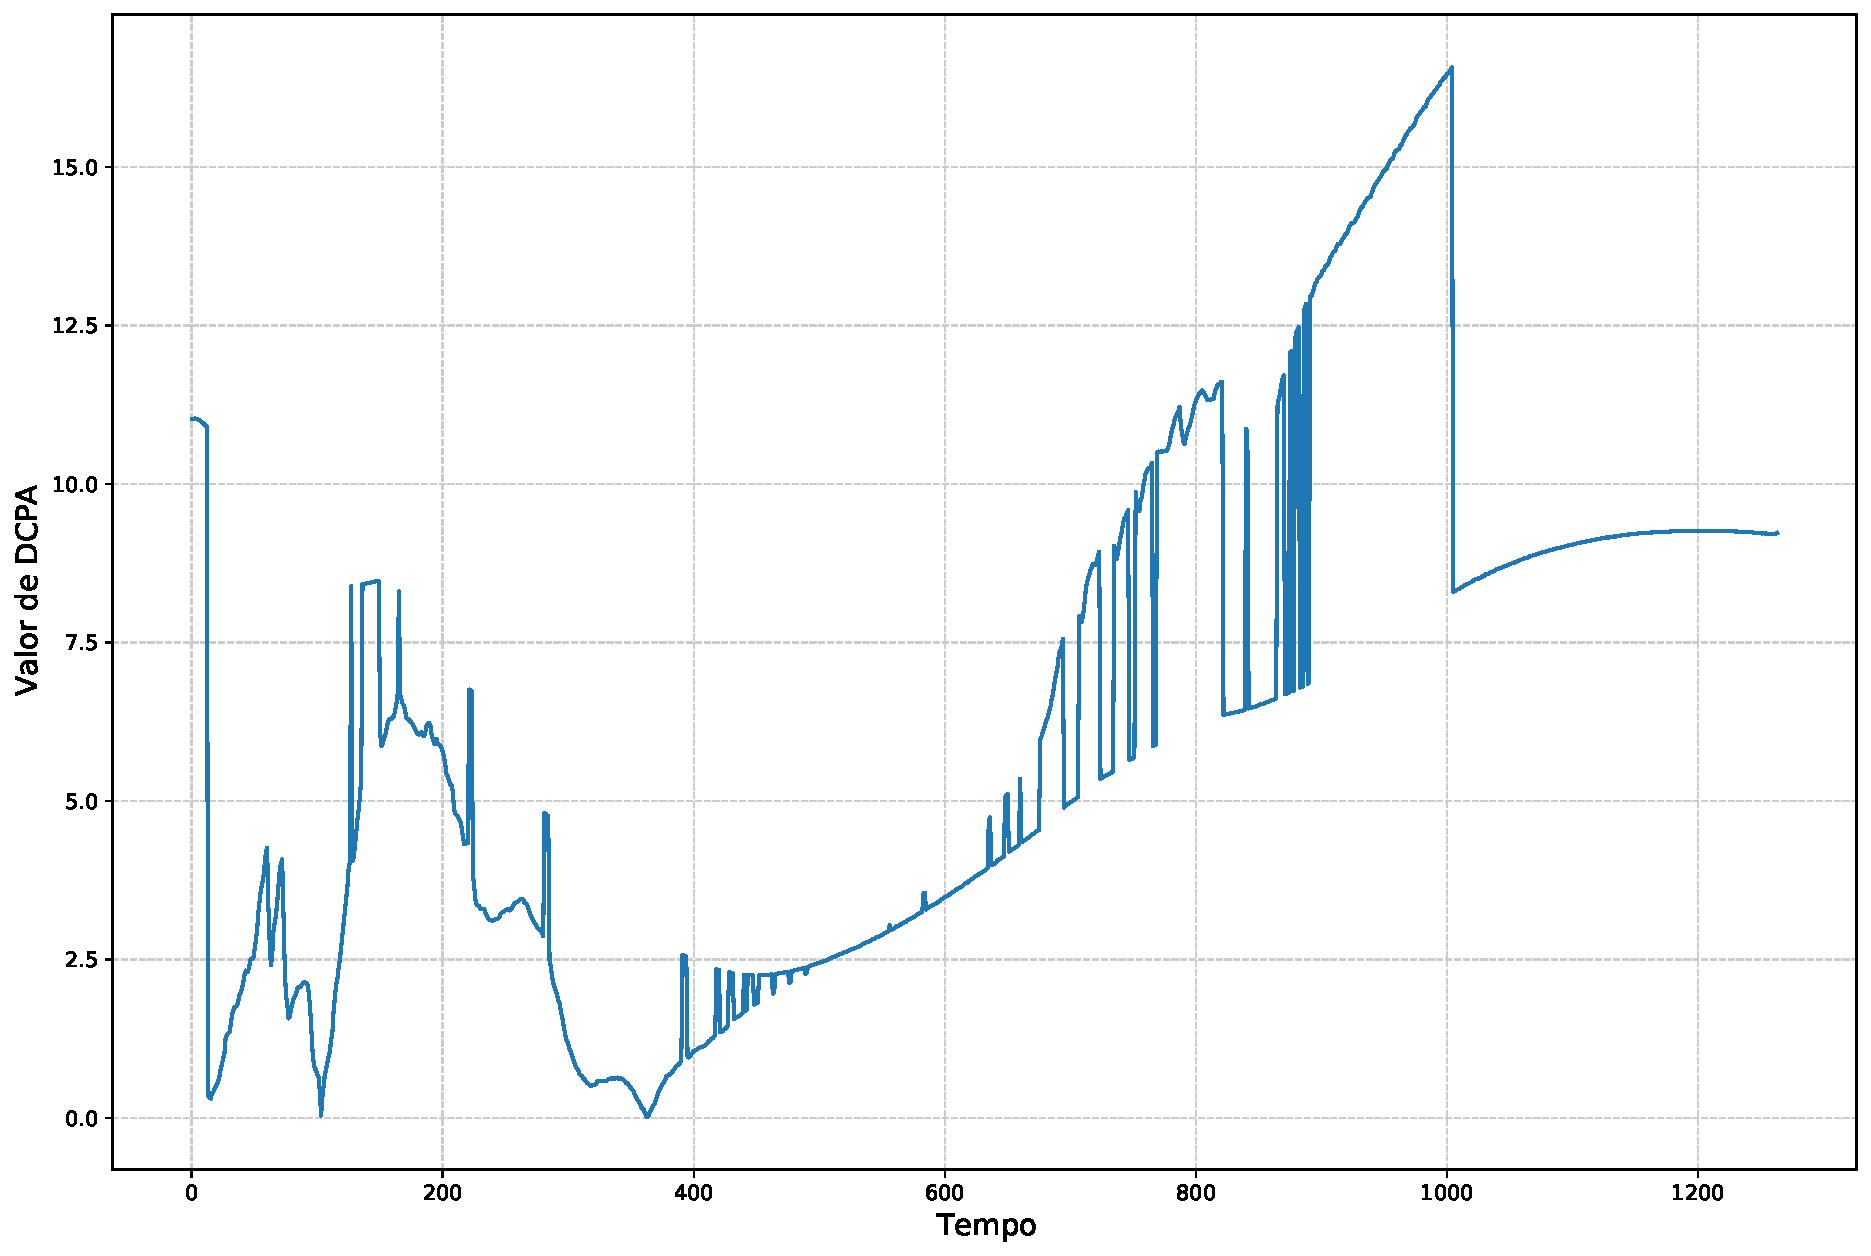
\includegraphics[width=\textwidth]{fig/chap5/overtake_dcpa.pdf}
            \caption{DCPA}
            \label{fig:chap5_overtake_dcpa}
        \end{subfigure}
        
        \caption{Informações do CPA}
        \label{fig:chap5_overtake_cpa}
        \end{figure}
        
        \begin{figure}[H]
            \centering
            % 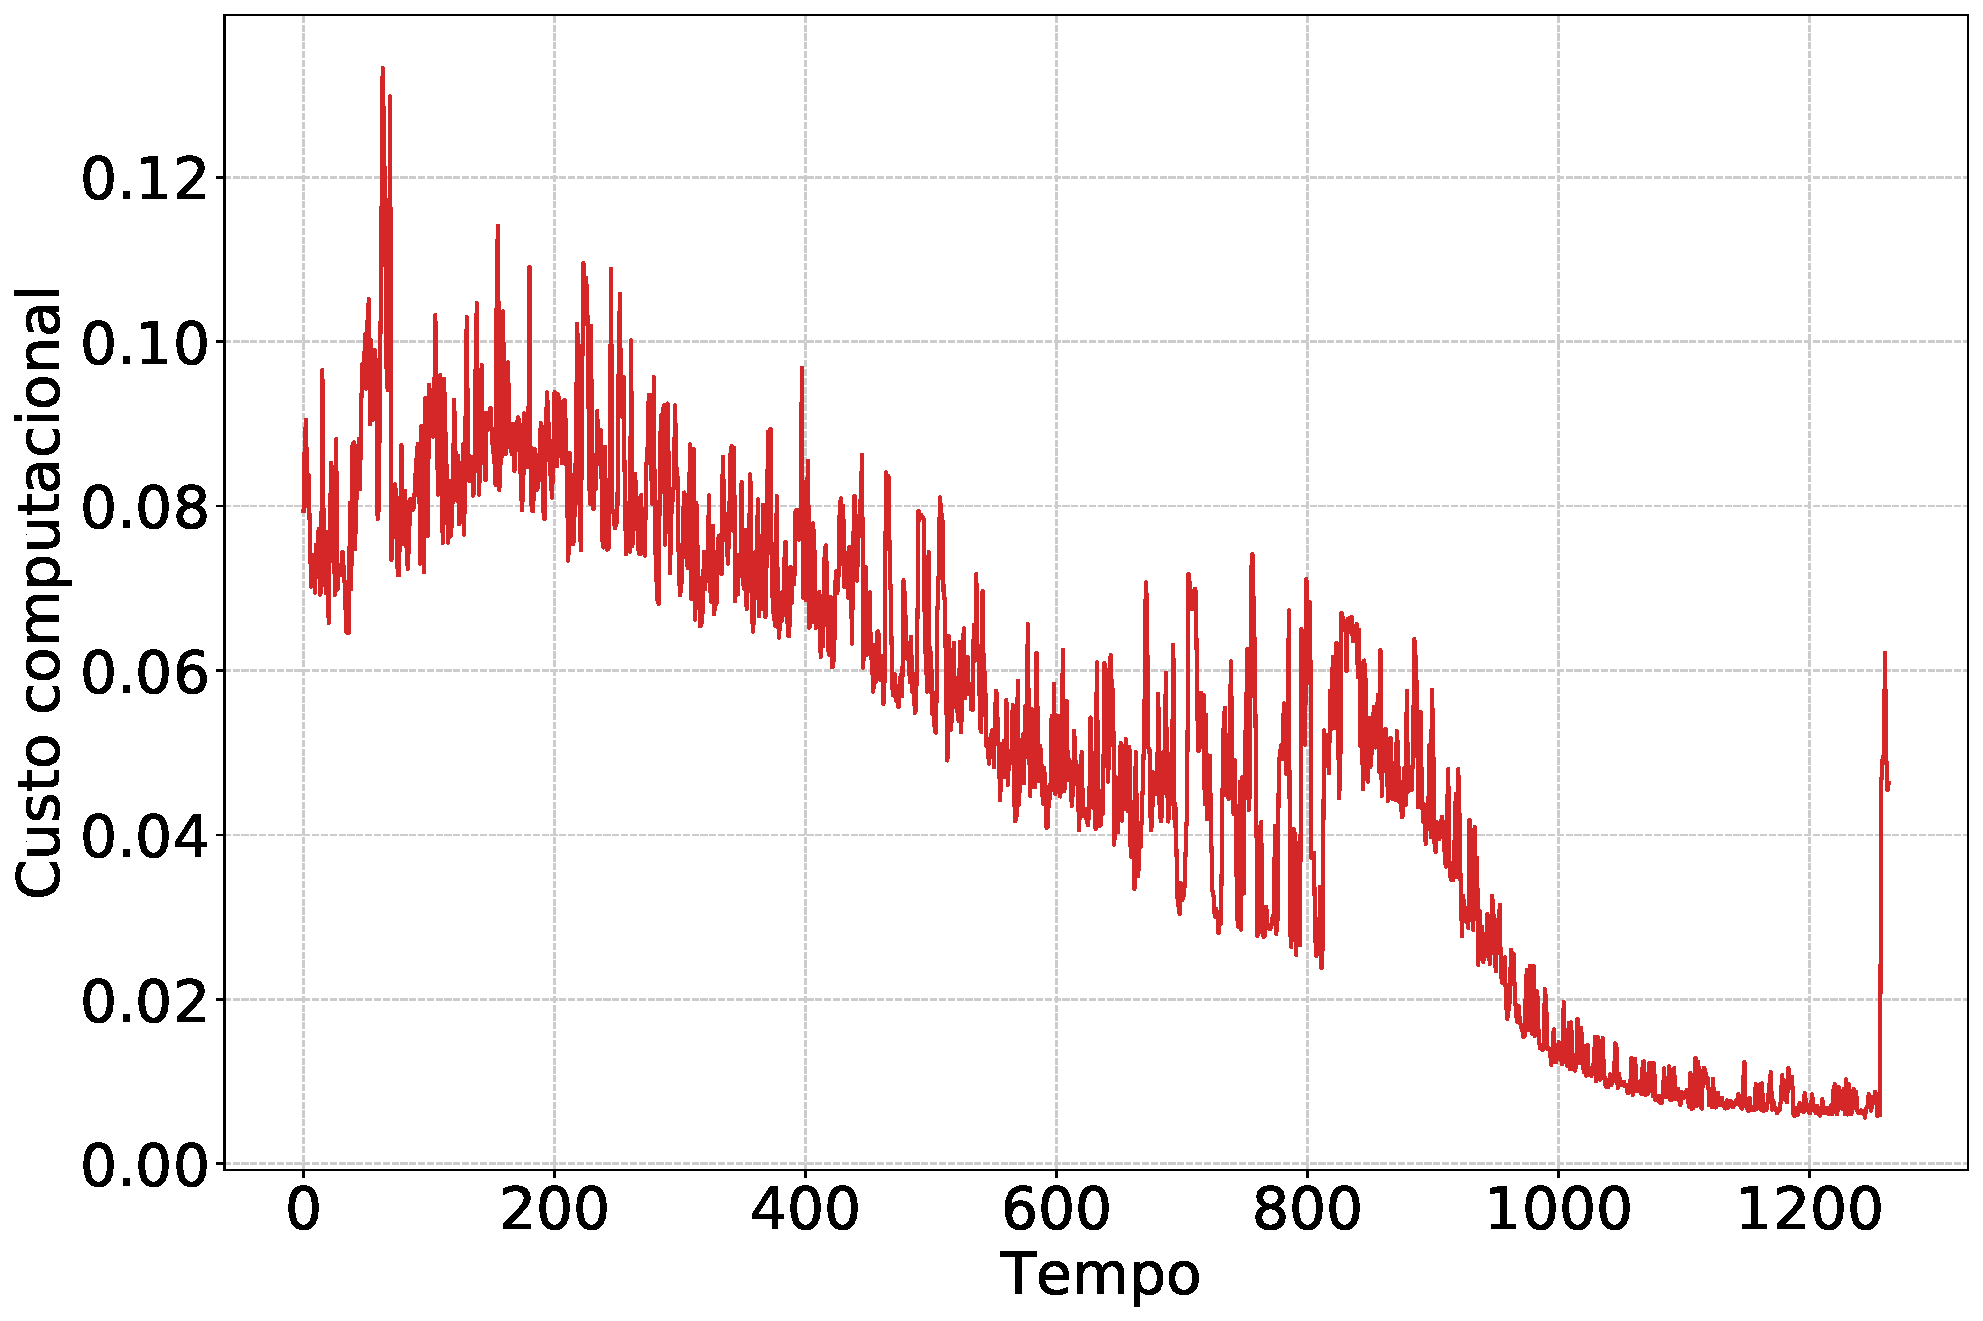
\includegraphics[width=0.3\textwidth]{fig/chap5/overtake_computation_time.pdf}
            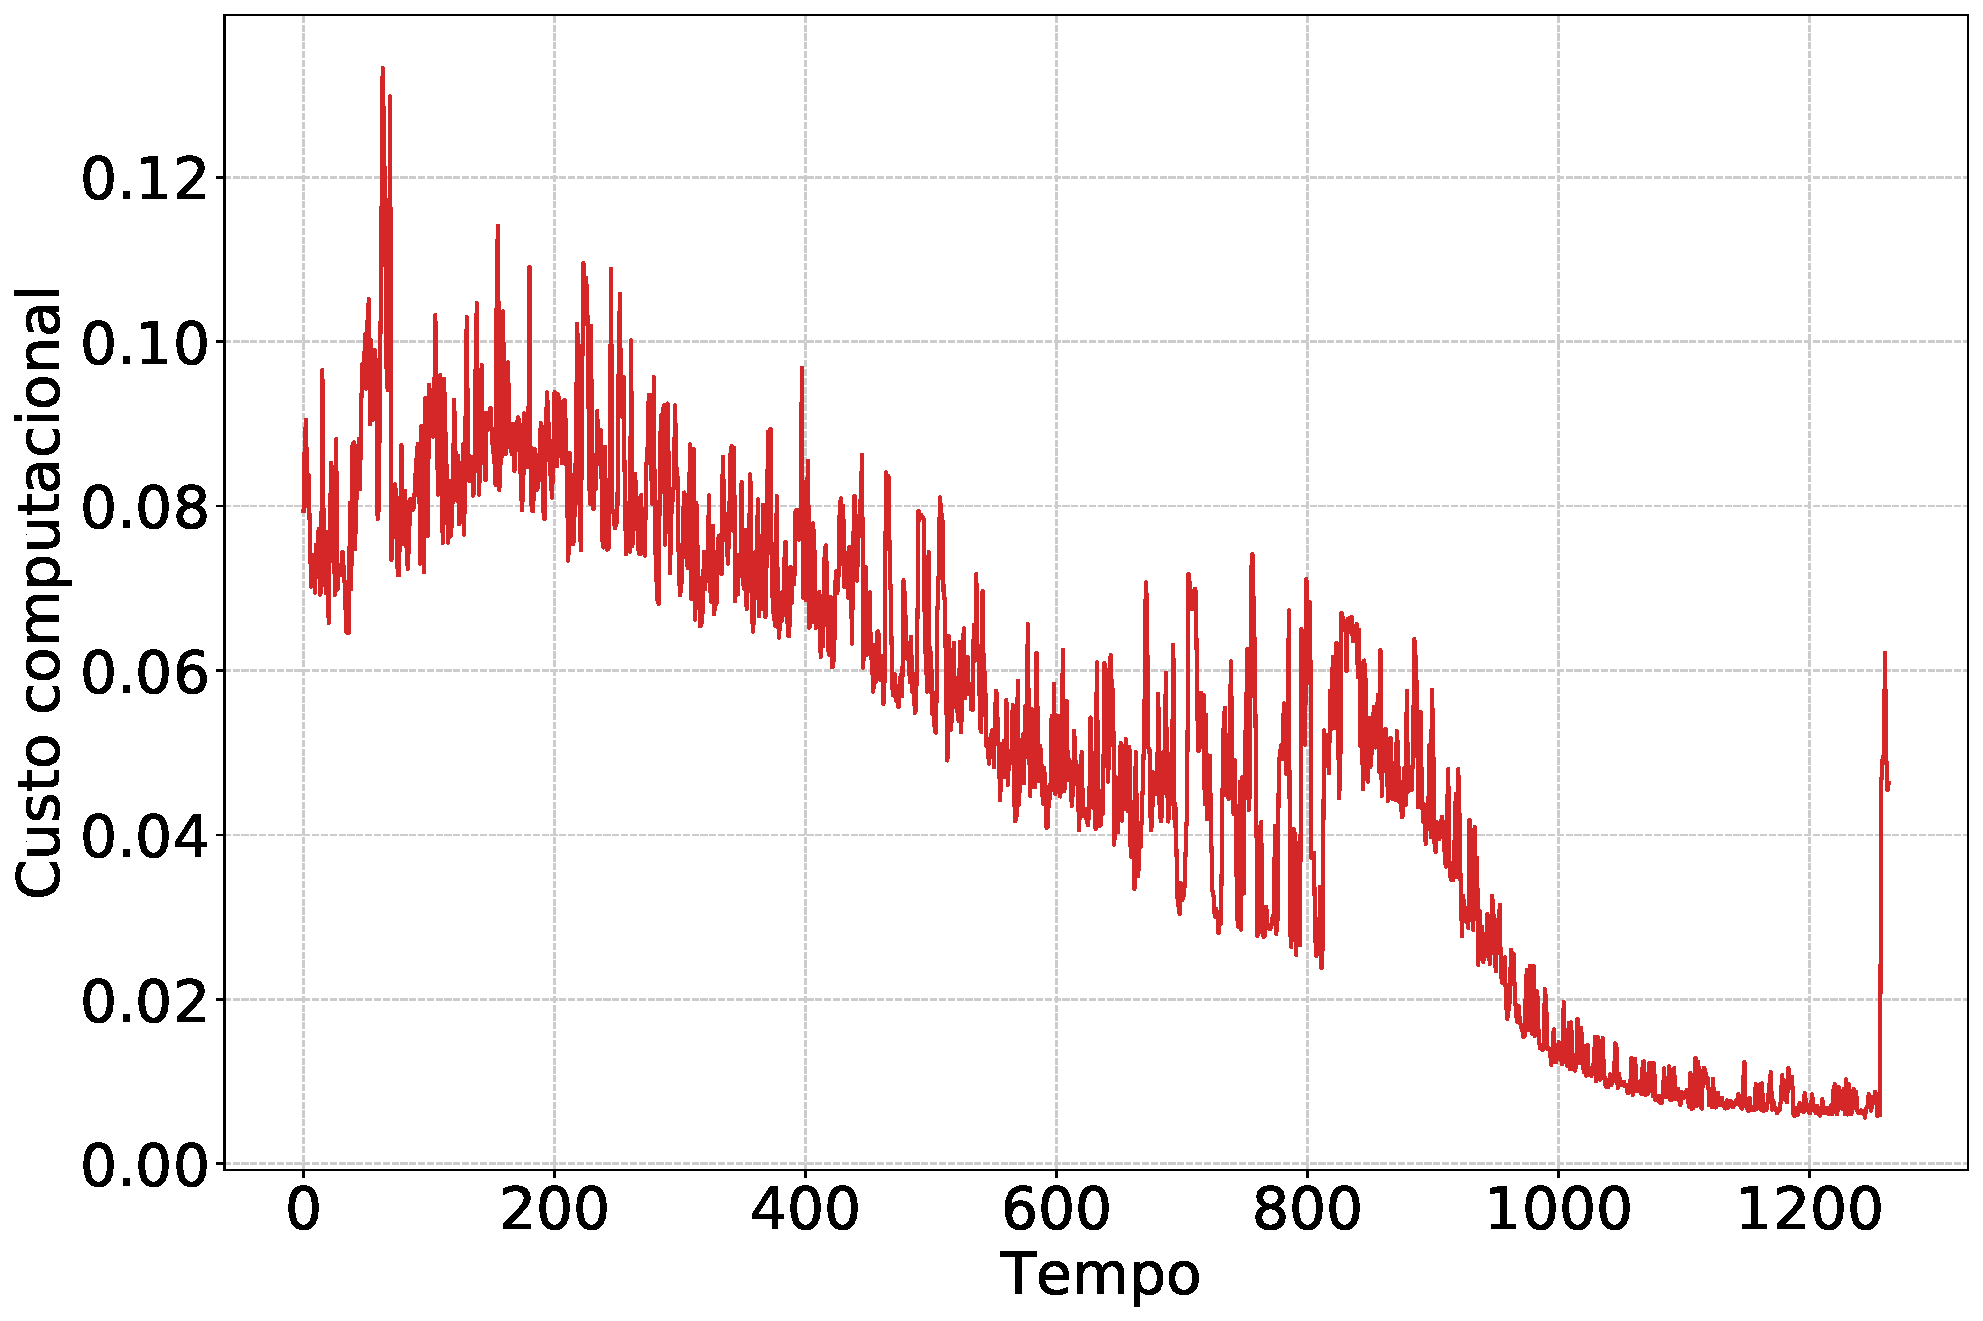
\includegraphics[width=\textwidth]{fig/chap5/overtake_computation_time.pdf}
            \caption{Tempo de computação}
            \label{fig:chap5_overtake_computation_time}
        \end{figure}
        
    \section{Crossing from Left} \label{subchap5_crossing_from_left}
        A Figura~\ref{fig:chap5_crossing_left_paths} mostra a trajetória resultante das embarcações para o caso de teste \textit{"Crossing from Left"}, onde o USV encontra a outra embarcação à sua esquerda. Nesse caso, segundo a COLREGS, o USV não é responsável por evitar a colisão em caso de risco. Novamente, a linha azul na Figura~\ref{fig:chap5_crossing_left_paths} indica o trajeto realizado pelo USV enquanto que a linha vermelha indica o trajeto realizado pela outra embarcação. Neste caso de teste a menor distância registrada entre as embarcações, indicado pelos triângulos vermelhos, foi de 8,316m. As análises do \tcpa e do \dcpa, ilustrados respectivamente na 
        Figura~\ref{fig:chap5_crossing_left_tcpa} e na Figura~\ref{fig:chap5_crossing_left_dcpa}, são análogas às análises realizadas anteriormente, em que com as embarcações se aproximando a tendência é que o \tcpa e o \dcpa diminuam, enquanto que ao se afastarem esses valores tendem a aumentar. No gráfico do tempo de computação (Figura~\ref{fig:chap5_crossing_left_computation_time}), percebe-se que o esforço computacional é muito pequeno até o momento em que a outra embarcação é detectada pelo planejador local. Segundo Jurak~\cite{Jurak2020COLREGS}, um erro de conversão de coordenadas globais para locais ocasiona um objetivo inválido para o planejador local, ocasionando o vale apresentado na Figura~\ref{fig:chap5_crossing_left_computation_time}. Pois segundo o fluxograma apresentado no 
        Capítulo~\ref{chap4:desenvolvimento}, se o objetivo do planejador local for inválido por dois ciclos de processamento, o sistema não deve fazer nada.
    
        \begin{figure}[H]
            \centering
            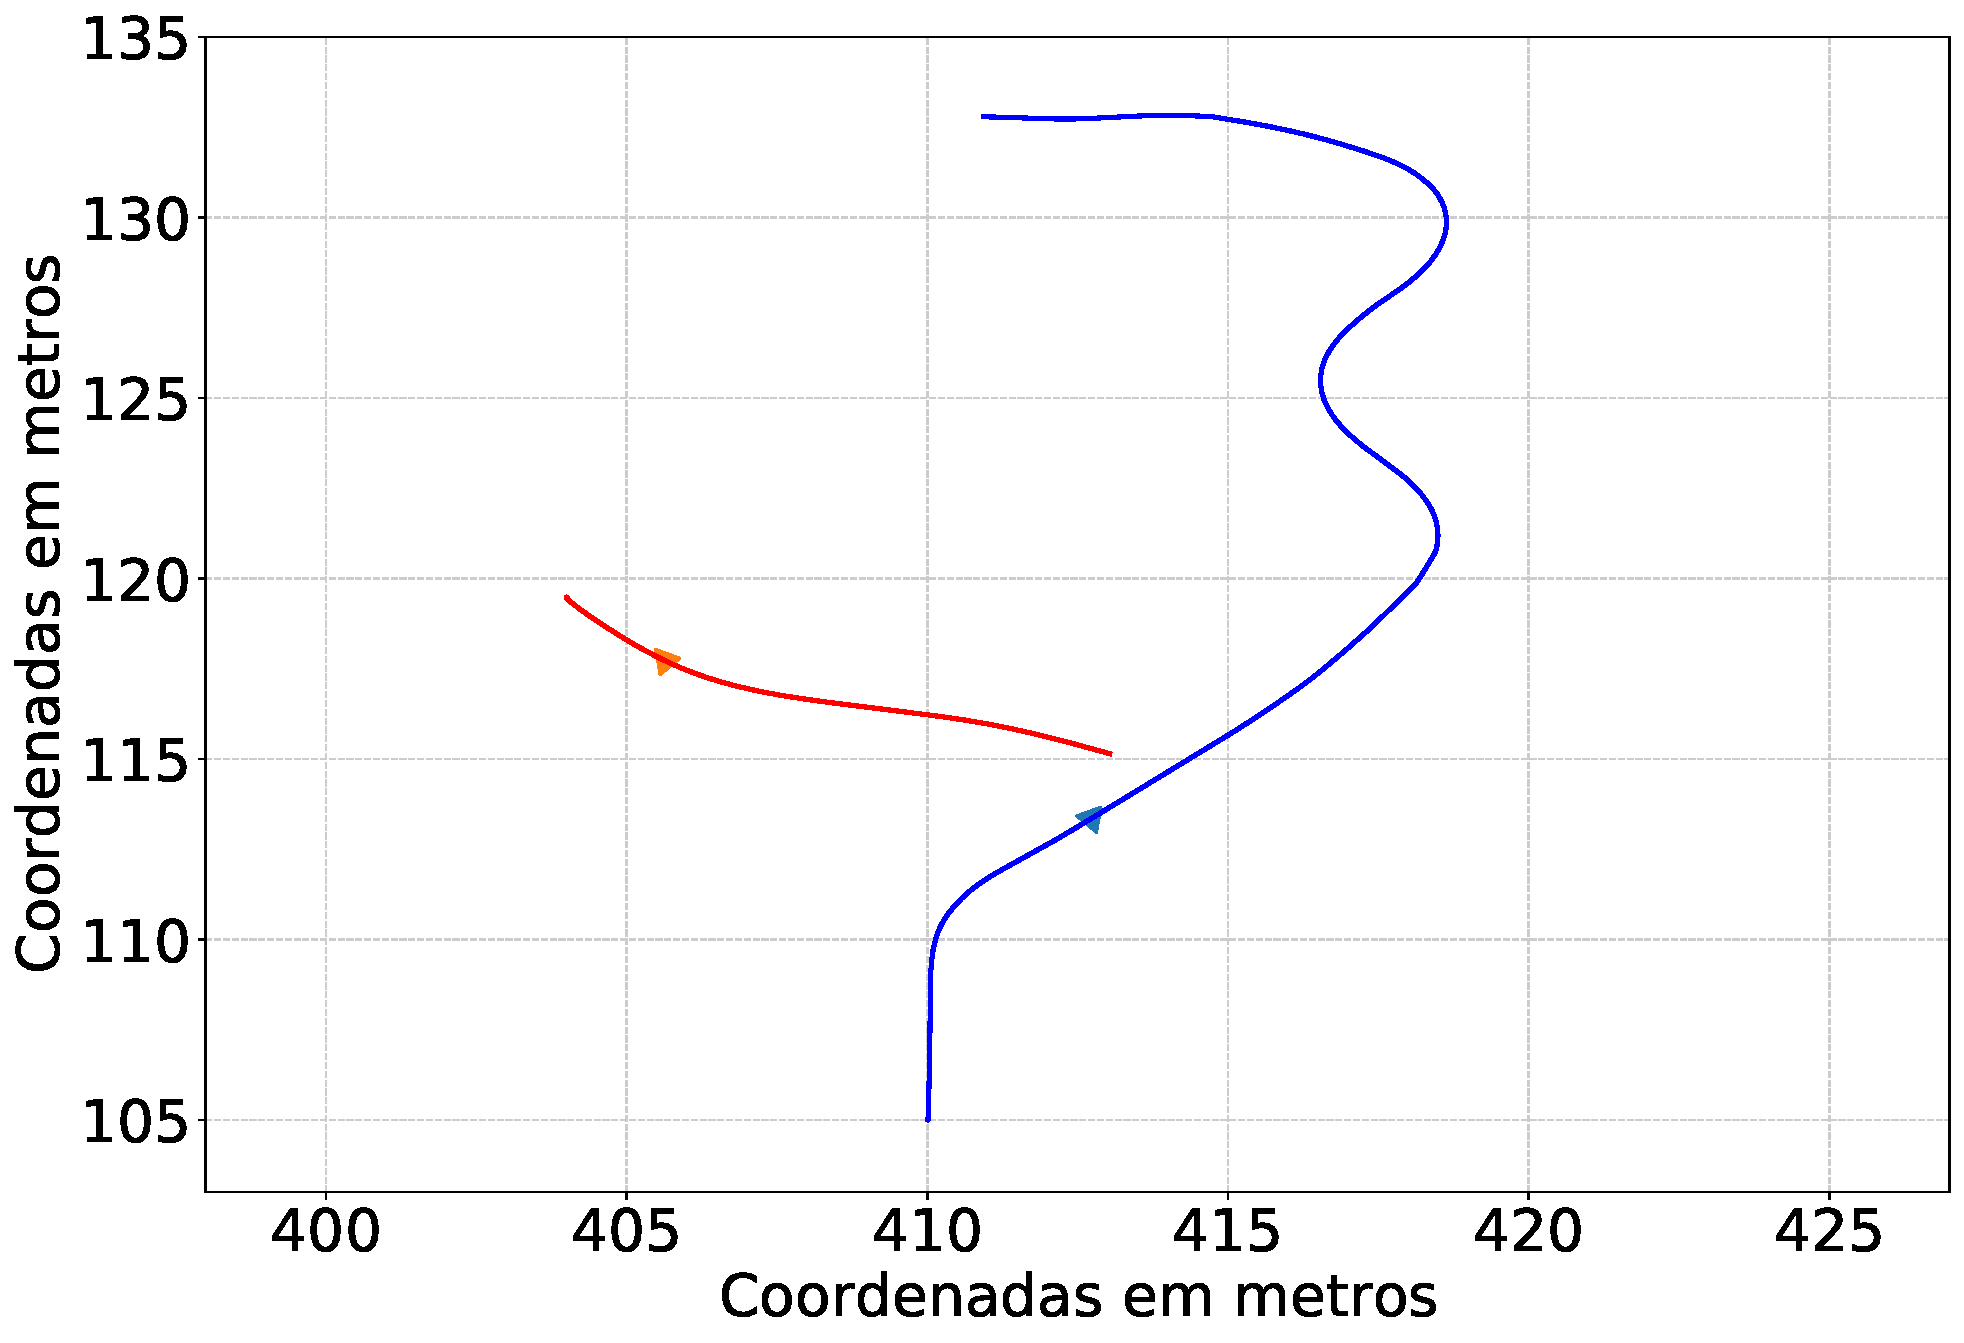
\includegraphics[scale=0.45]{fig/chap5/crossing_left_trajectory.pdf}
            \caption{Trajeto das embarcações}
            \label{fig:chap5_crossing_left_paths}
        \end{figure}
        
        \begin{figure}[H]
		\centering
% 		\begin{subfigure}{0.5\textwidth}
		\begin{subfigure}{1\textwidth}
            \centering
            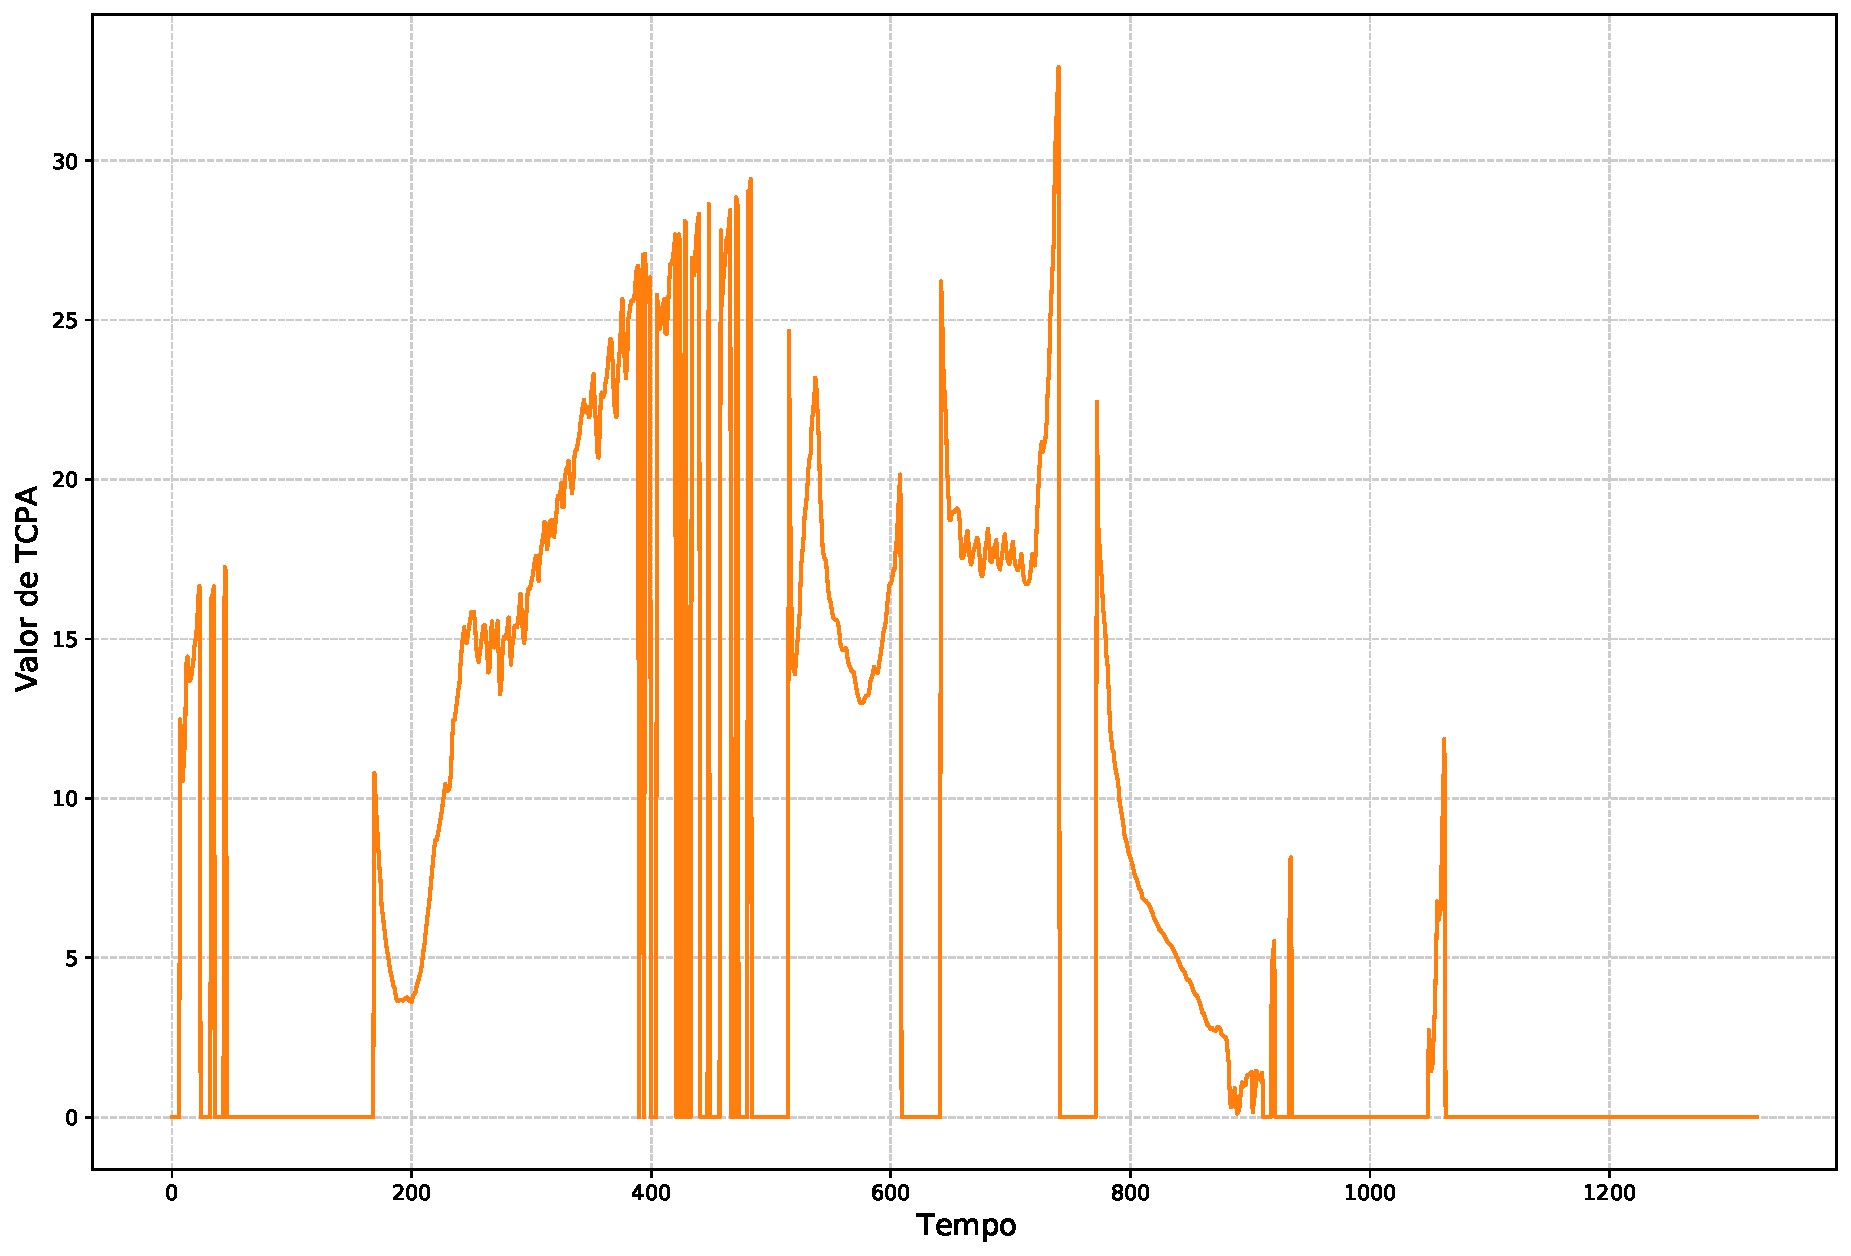
\includegraphics[width=\textwidth]{fig/chap5/crossing_left_tcpa.pdf}
            \caption{TCPA}
            \label{fig:chap5_crossing_left_tcpa}
        \end{subfigure}
        % \begin{subfigure}{0.5\textwidth}
        \begin{subfigure}{1\textwidth}
            \centering
            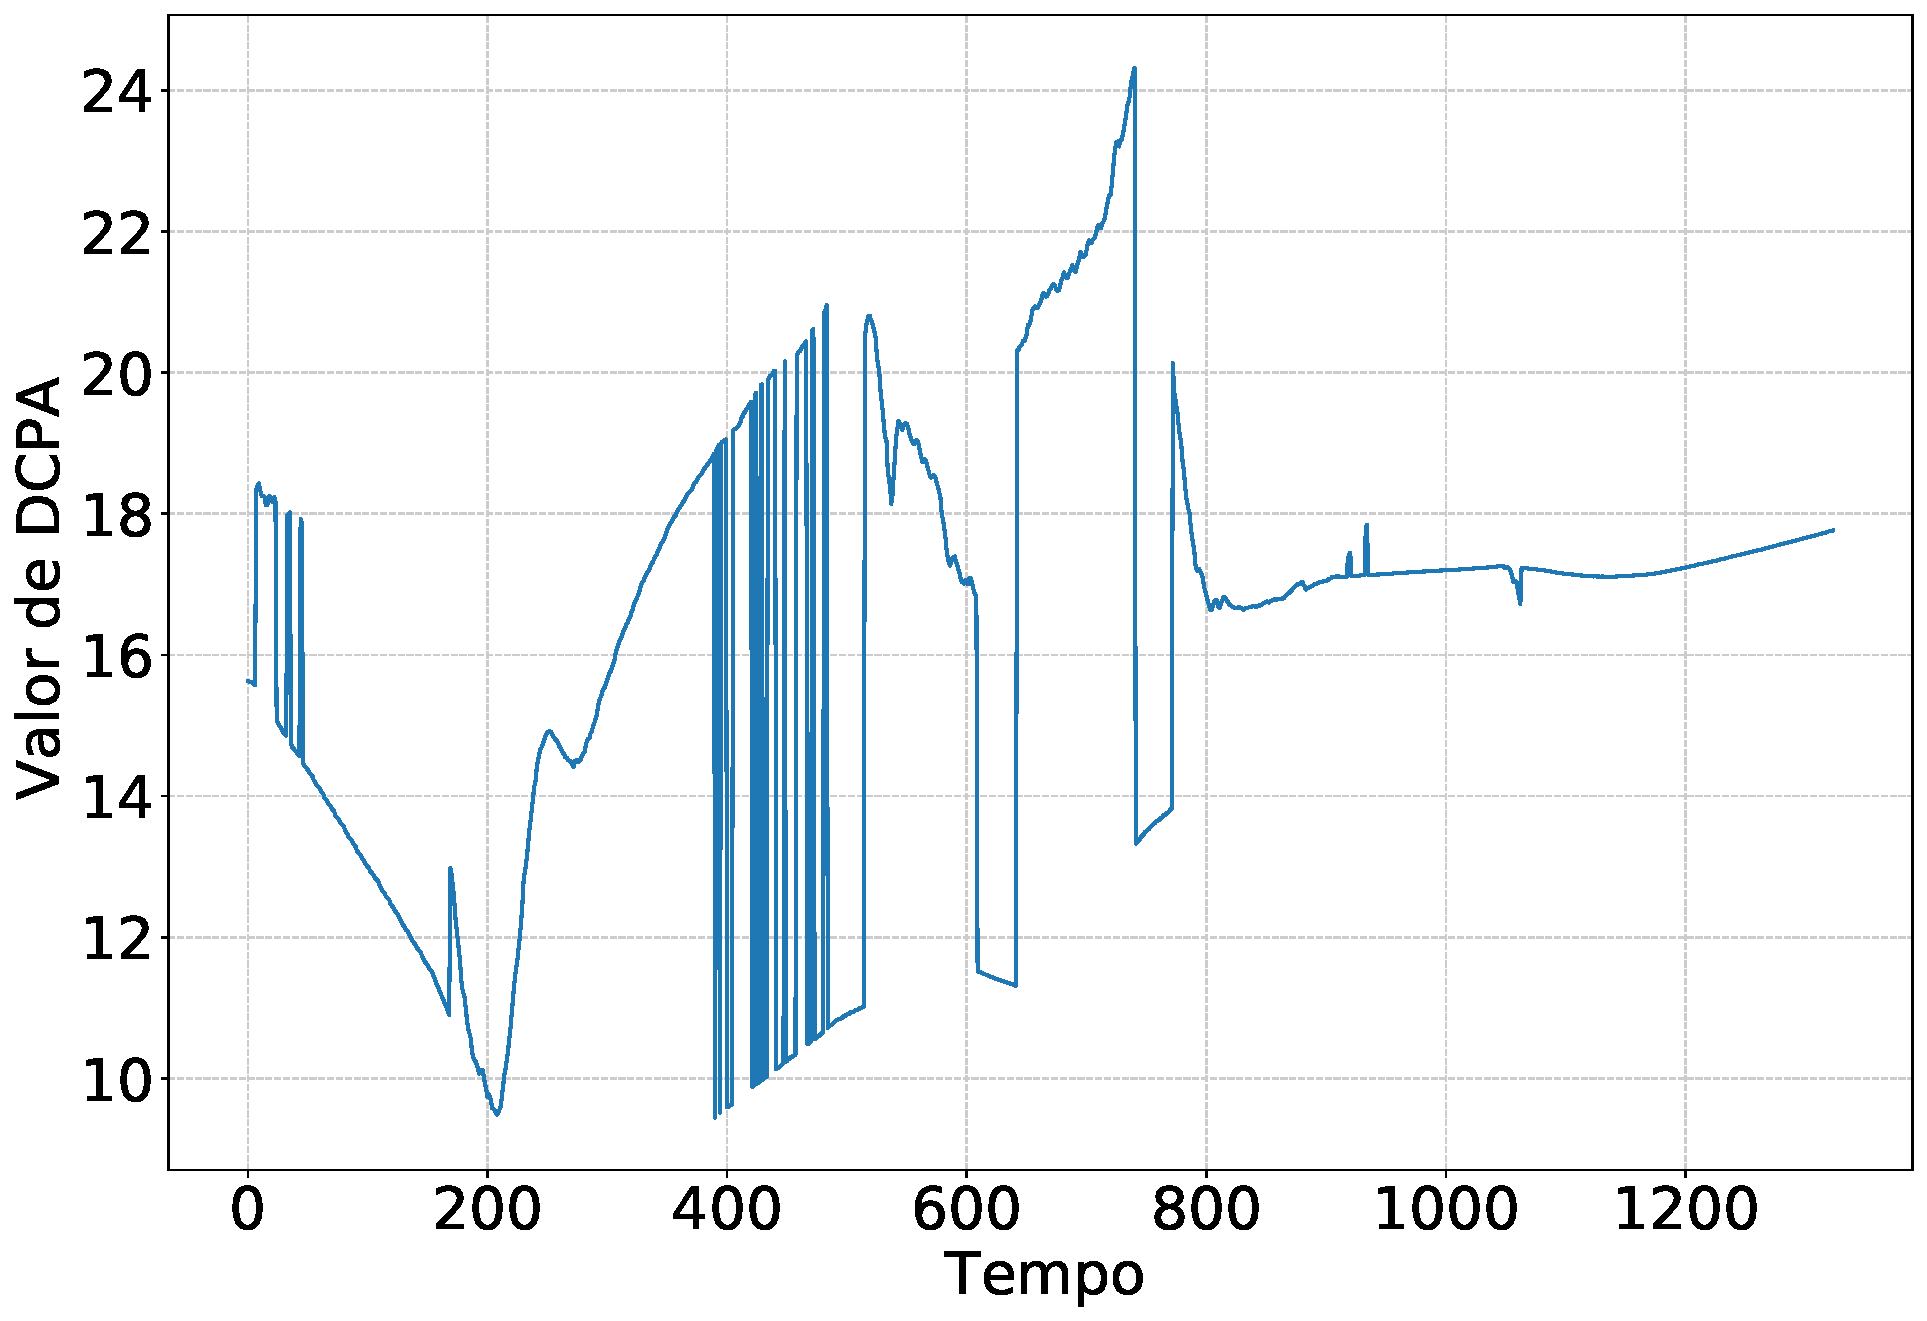
\includegraphics[width=\textwidth]{fig/chap5/crossing_left_dcpa.pdf}
            \caption{DCPA}
            \label{fig:chap5_crossing_left_dcpa}
        \end{subfigure}
        
        \caption{Informações do CPA}
        \label{fig:chap5_crossing_left_cpa}
        \end{figure}
        
        \begin{figure}[H]
            \centering
            % 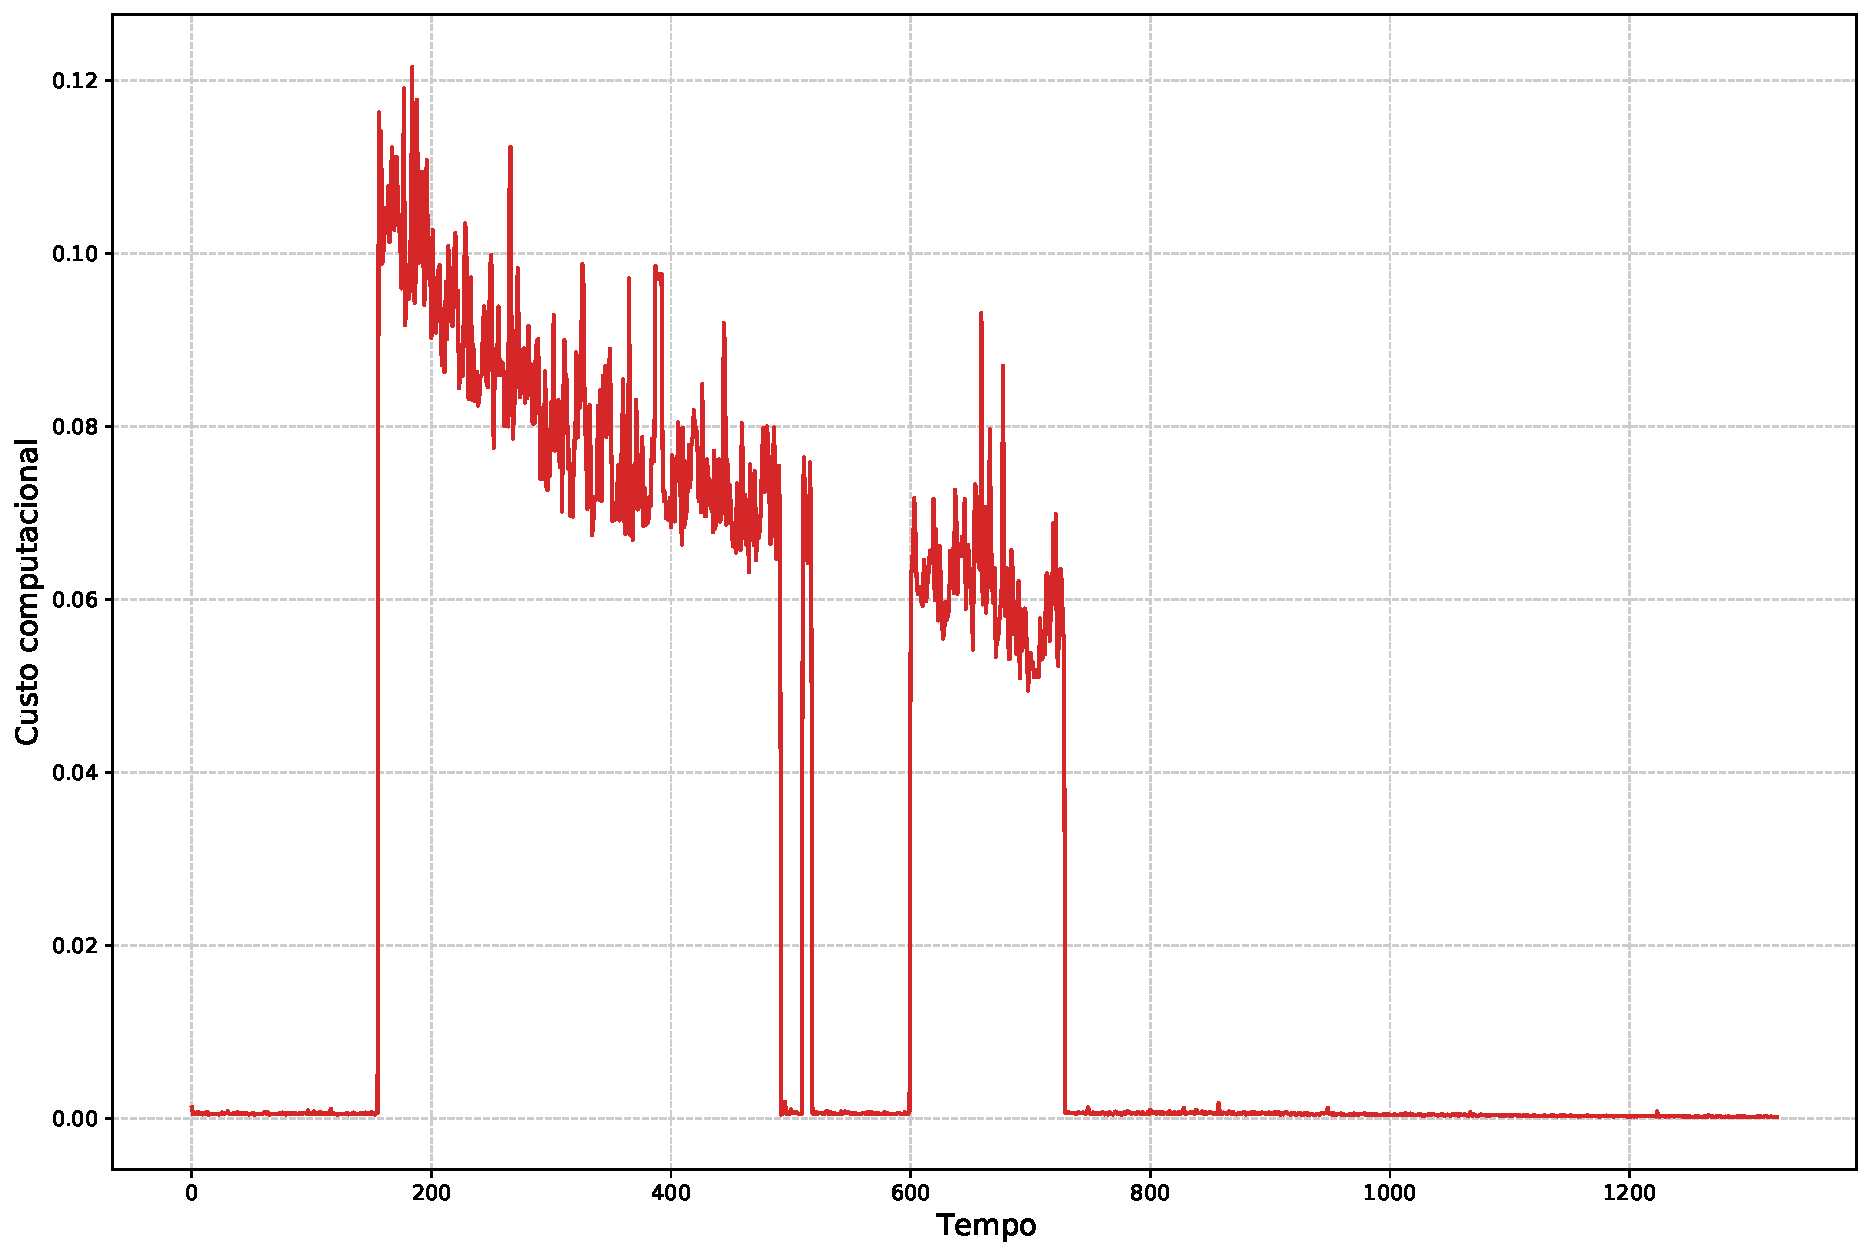
\includegraphics[scale=0.3]{fig/chap5/crossing_left_computation_time.pdf}
            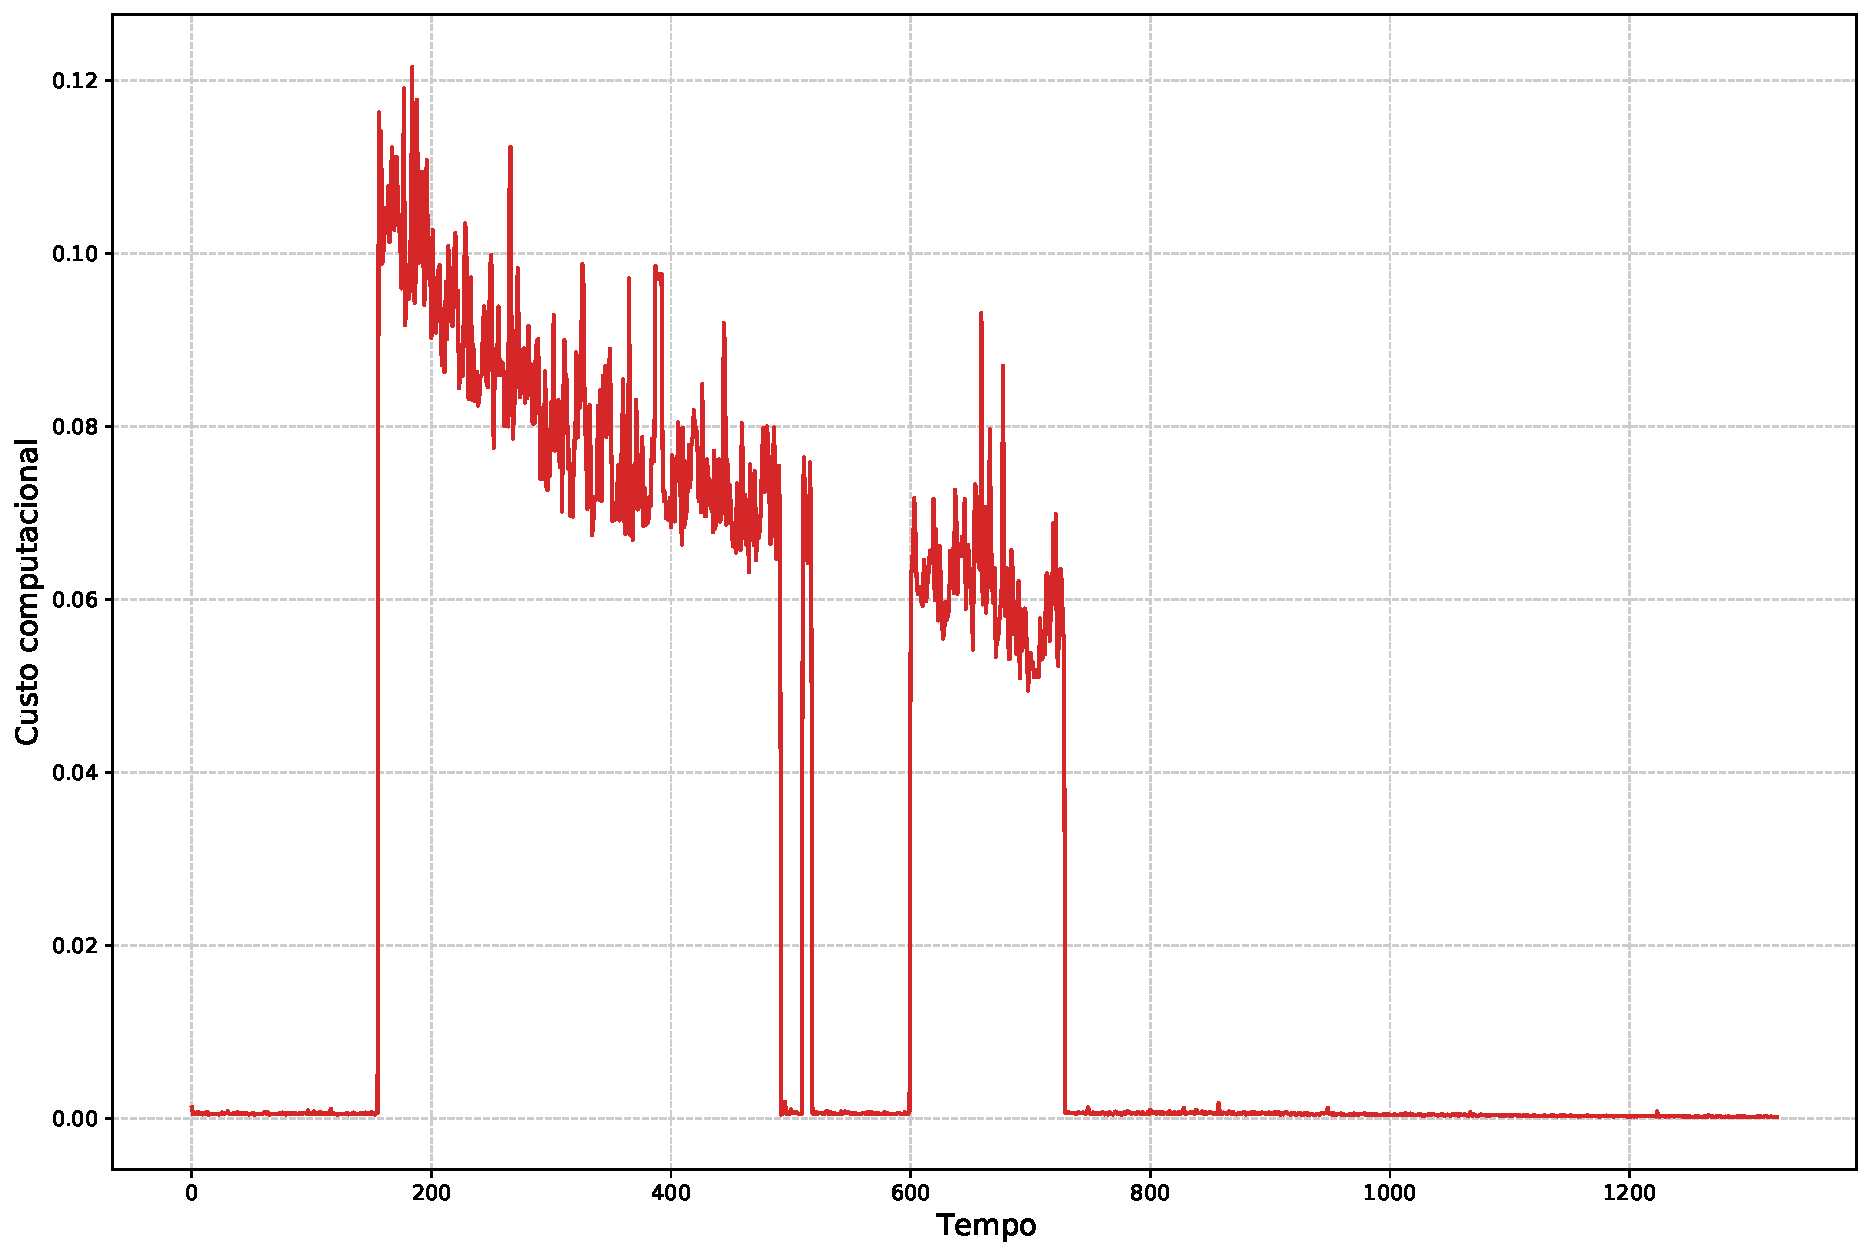
\includegraphics[width=\textwidth]{fig/chap5/crossing_left_computation_time.pdf}
            \caption{Tempo de computação}
            \label{fig:chap5_crossing_left_computation_time}
        \end{figure}
        
    \section{Crossing from Right} \label{subchap5_crossing_from_right}
        A Figura~\ref{fig:chap5_crossing_right_paths} apresenta a trajetória das embarcações para o presente caso de teste, onde o USV encontra a outra embarcação vindo pelo seu lado direito. Nesse caso o USV é responsável por evitar uma possível colisão, desviando de sua rota original pela direita a fim de passar por trás da outra embarcação. Novamente a linha azul representa o trajeto realizado pelo USV enquanto que a linha vermelha representa o trajeto da outra 
        embarcação. A menor distância registrada nesse teste foi de 1,866m e a posição das embarcações nesse momento está indicada pelos triângulos em cada linha na imagem. A análise do \tcpa e do \dcpa, ilustrados respectivamente pela Figura~\ref{fig:chap5_crossing_right_tcpa} e Figura~\ref{fig:chap5_crossing_right_dcpa}, são análogas às análises anteriores. Ou seja, conforme as embarcações vão se aproximando menor é o \tcpa e \dcpa calculado, conforme a distância entre as embarcações vai aumentando a tendência é que o \tcpa e o \dcpa também aumentem em decorrência da distância. O tempo de computação, ilustrado pela Figura~\ref{fig:chap5_crossing_right_computation_time}, tem seus picos justificados pelo planejamento necessário enquanto a outra embarcação estiver no alcance do planejador local.
    
        \begin{figure}[H]
            \centering
            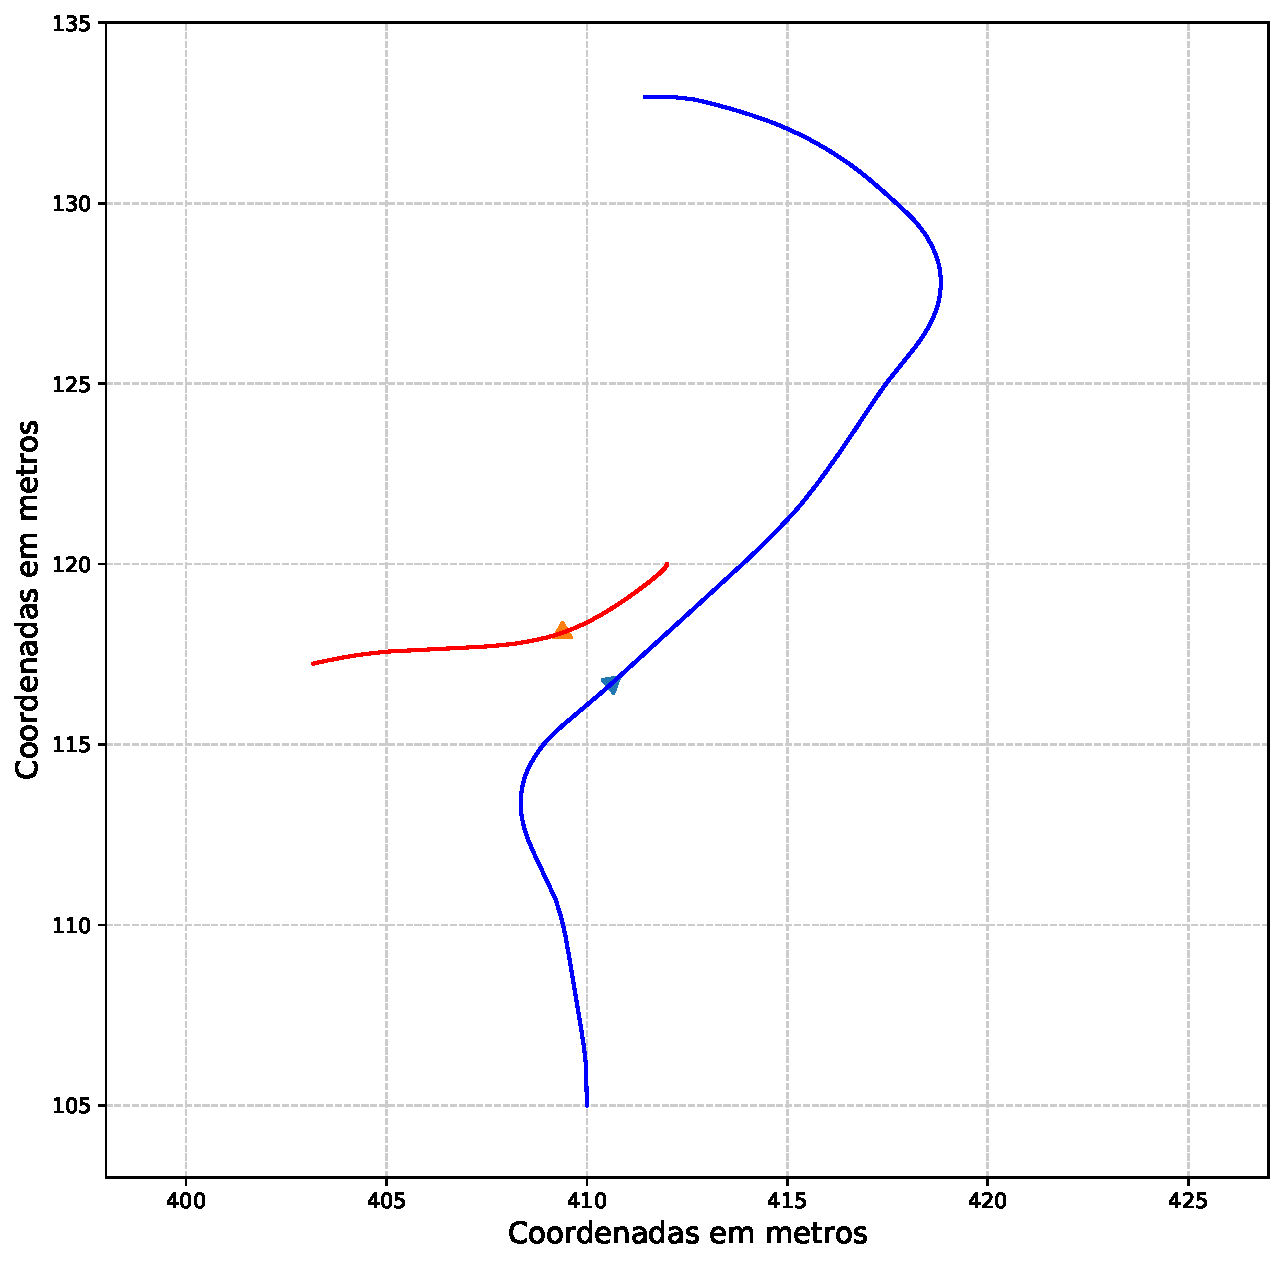
\includegraphics[scale=0.45]{fig/chap5/crossing_right_trajectory.pdf}
            \caption{Trajeto das embarcações}
            \label{fig:chap5_crossing_right_paths}
        \end{figure}
        
        \begin{figure}[H]
		\centering
% 		\begin{subfigure}{0.5\textwidth}
		\begin{subfigure}{1\textwidth}
            \centering
            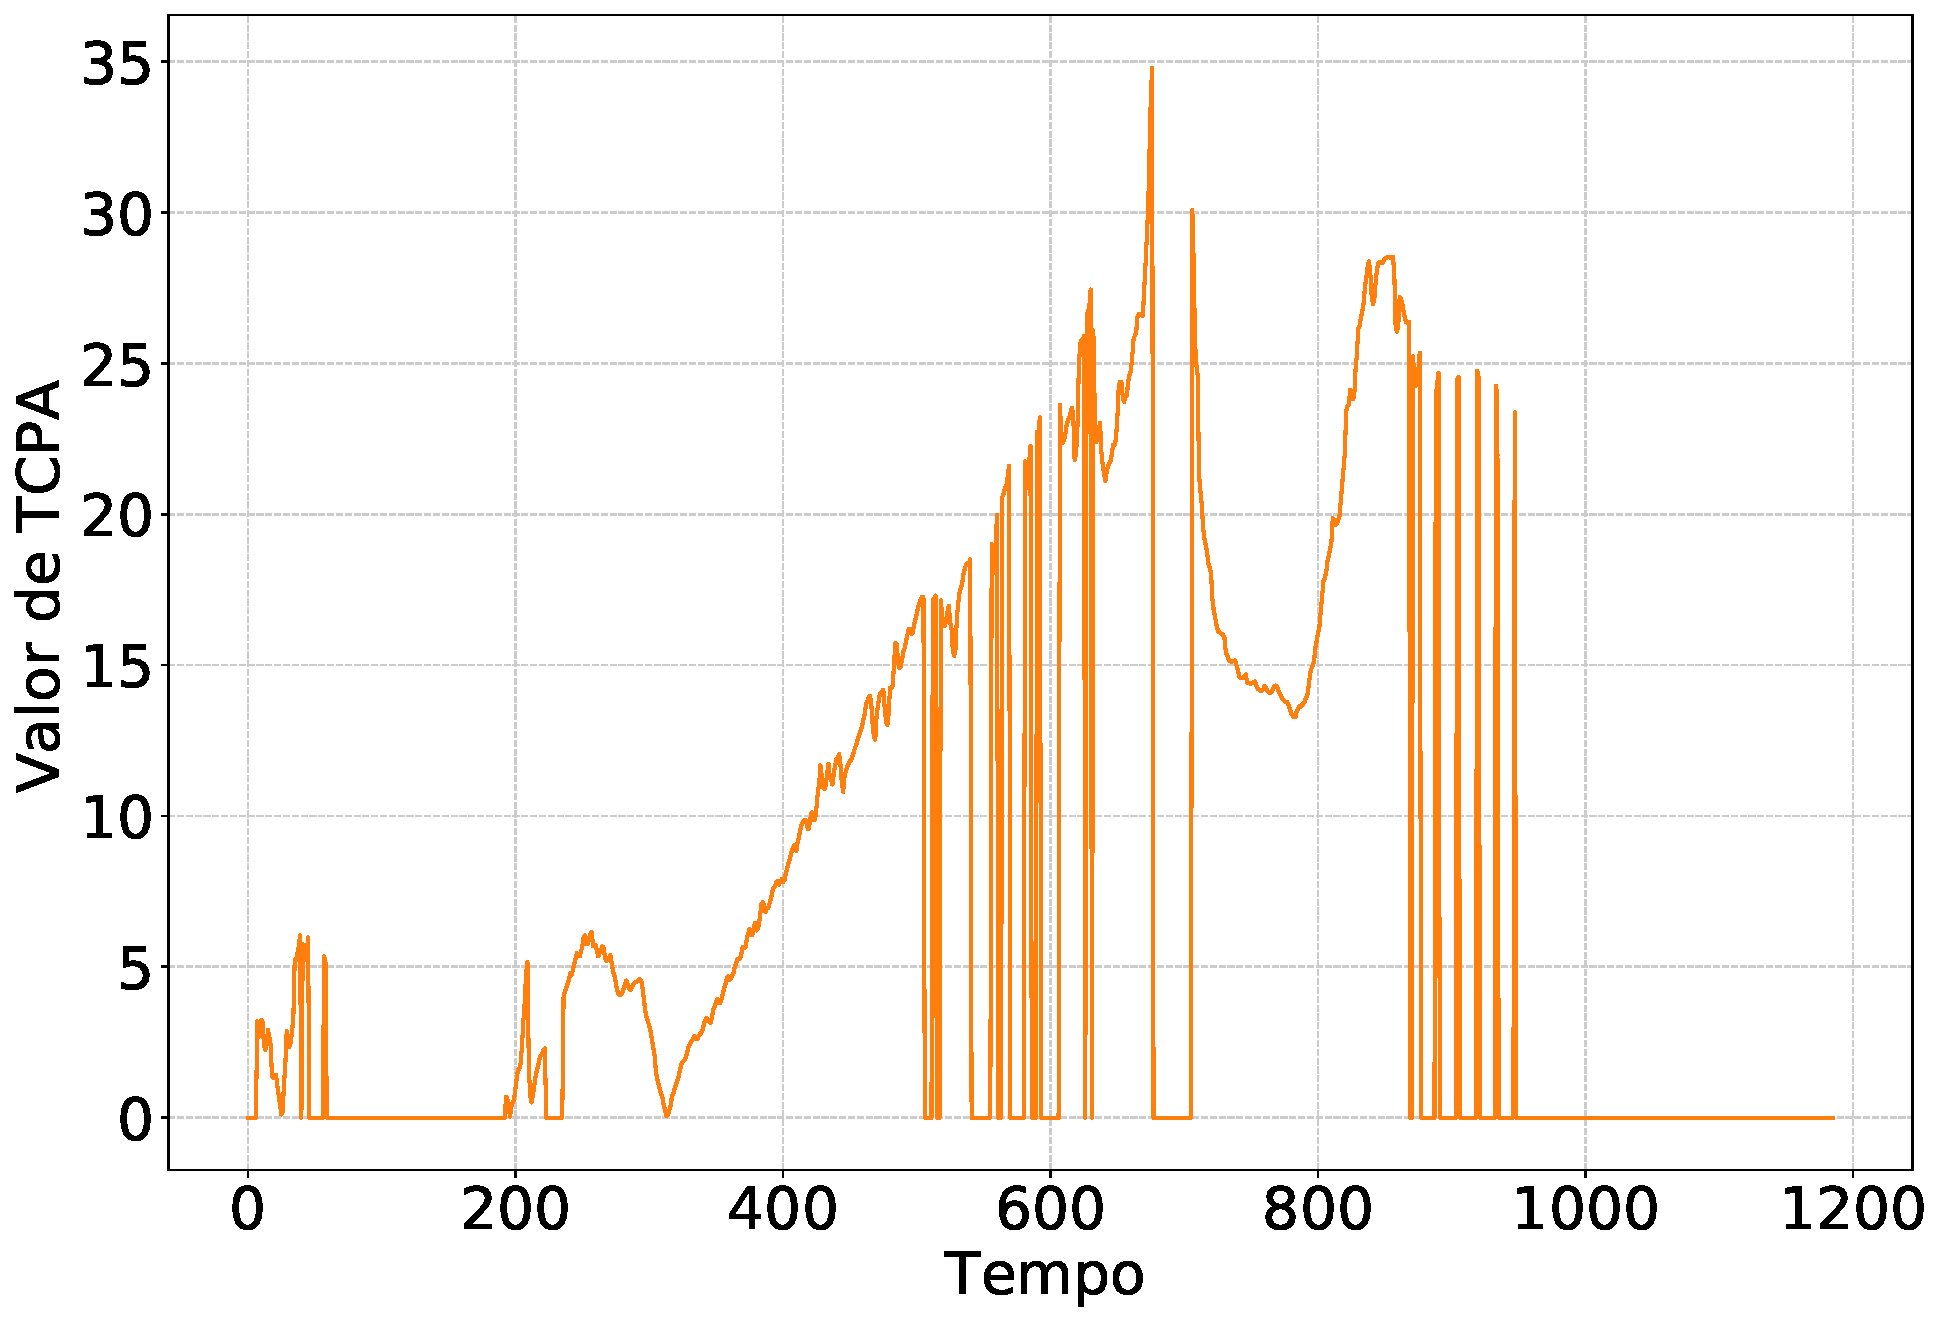
\includegraphics[width=\textwidth]{fig/chap5/crossing_right_tcpa.pdf}
            \caption{TCPA}
            \label{fig:chap5_crossing_right_tcpa}
        \end{subfigure}
        % \begin{subfigure}{0.5\textwidth}
        \begin{subfigure}{1\textwidth}
            \centering
            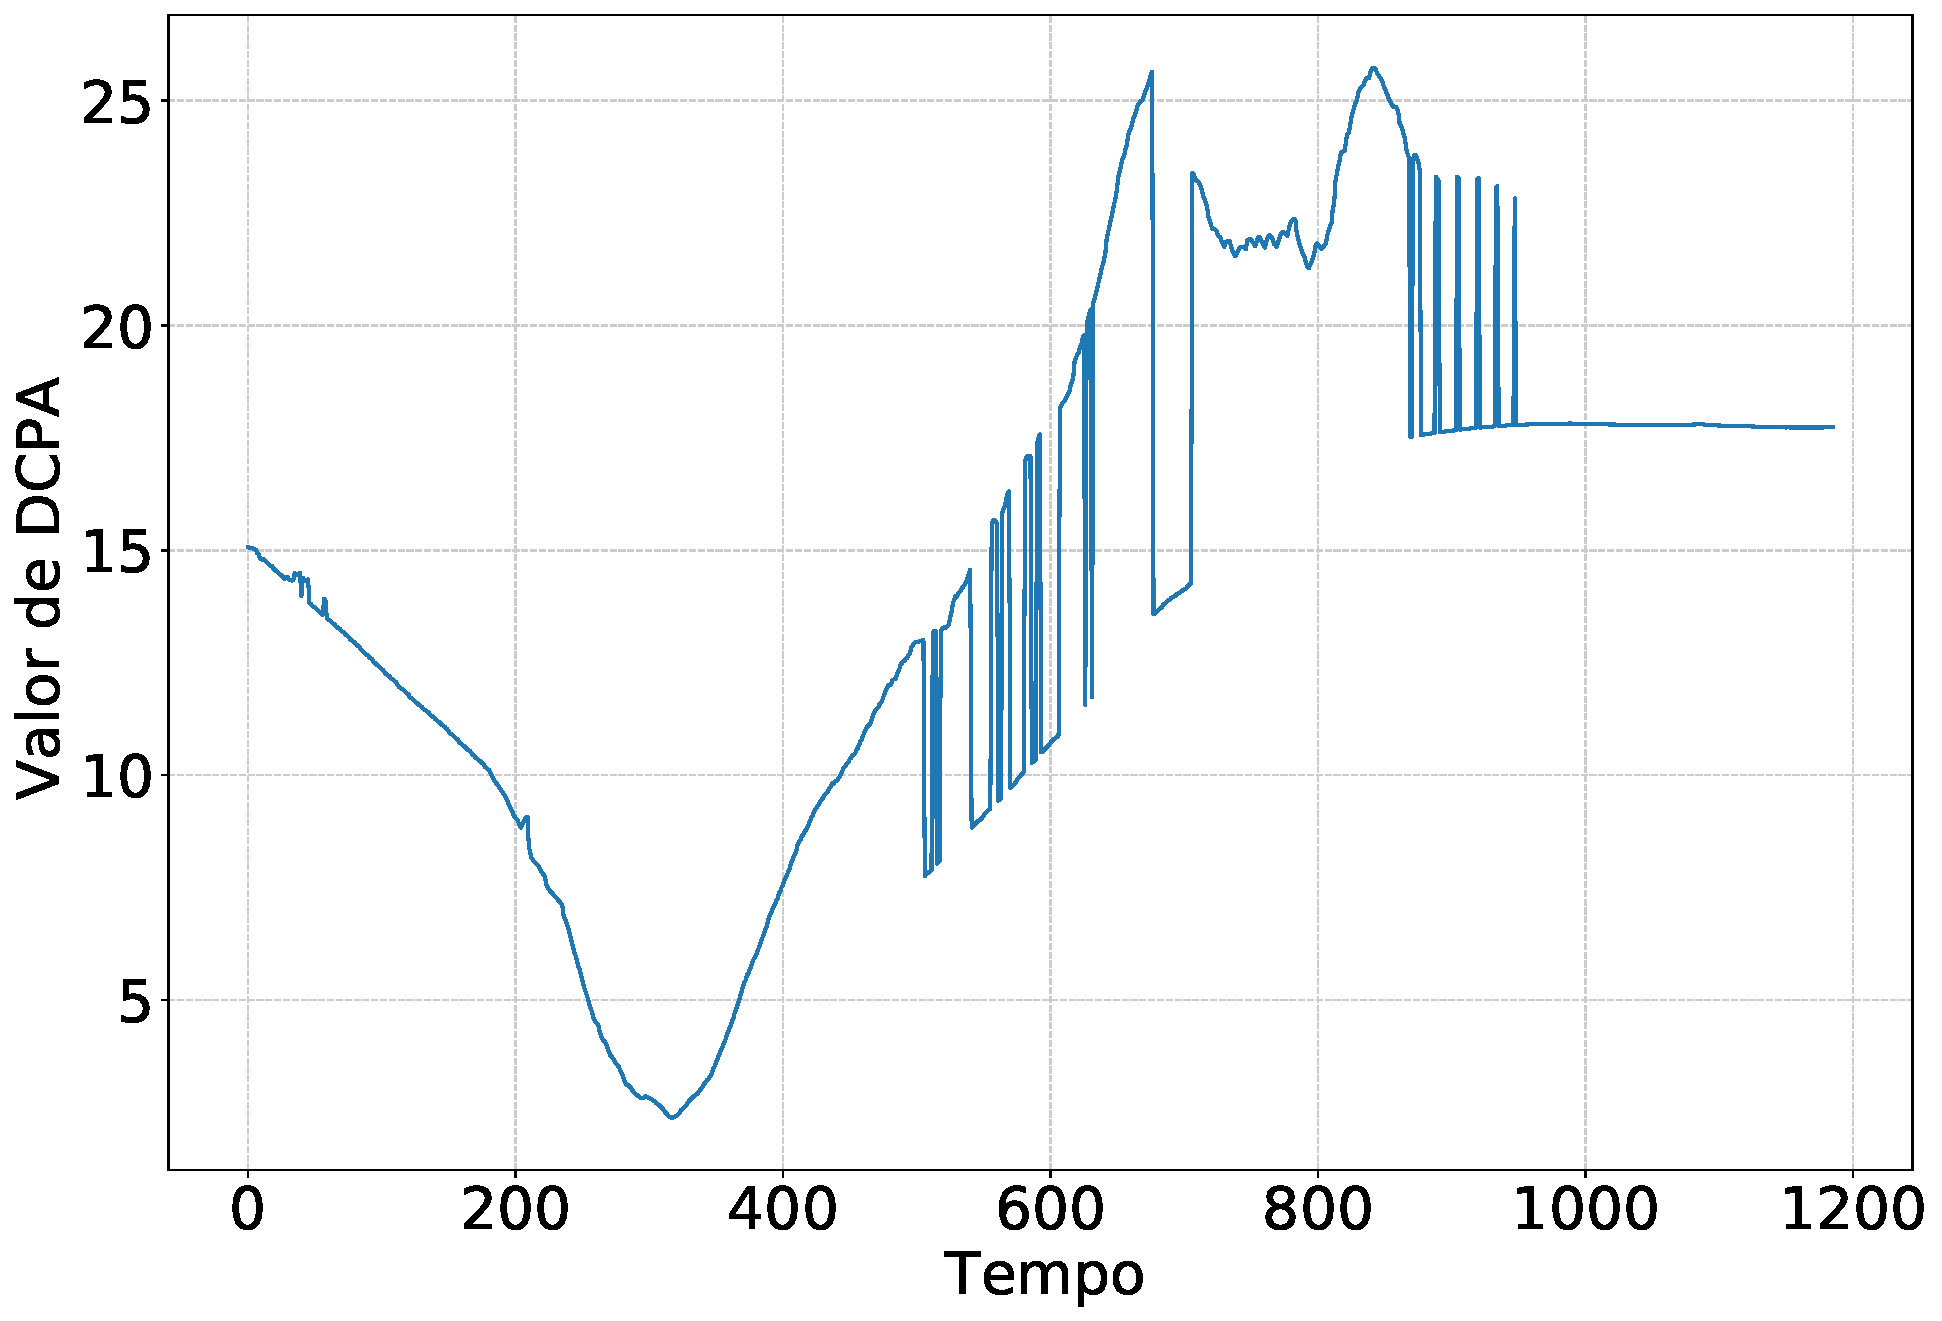
\includegraphics[width=\textwidth]{fig/chap5/crossing_right_dcpa.pdf}
            \caption{DCPA}
            \label{fig:chap5_crossing_right_dcpa}
        \end{subfigure}
        
        \caption{Informações do CPA}
        \label{fig:chap5_crossing_right_cpa}
        \end{figure}
        
        \begin{figure}[H]
            \centering
            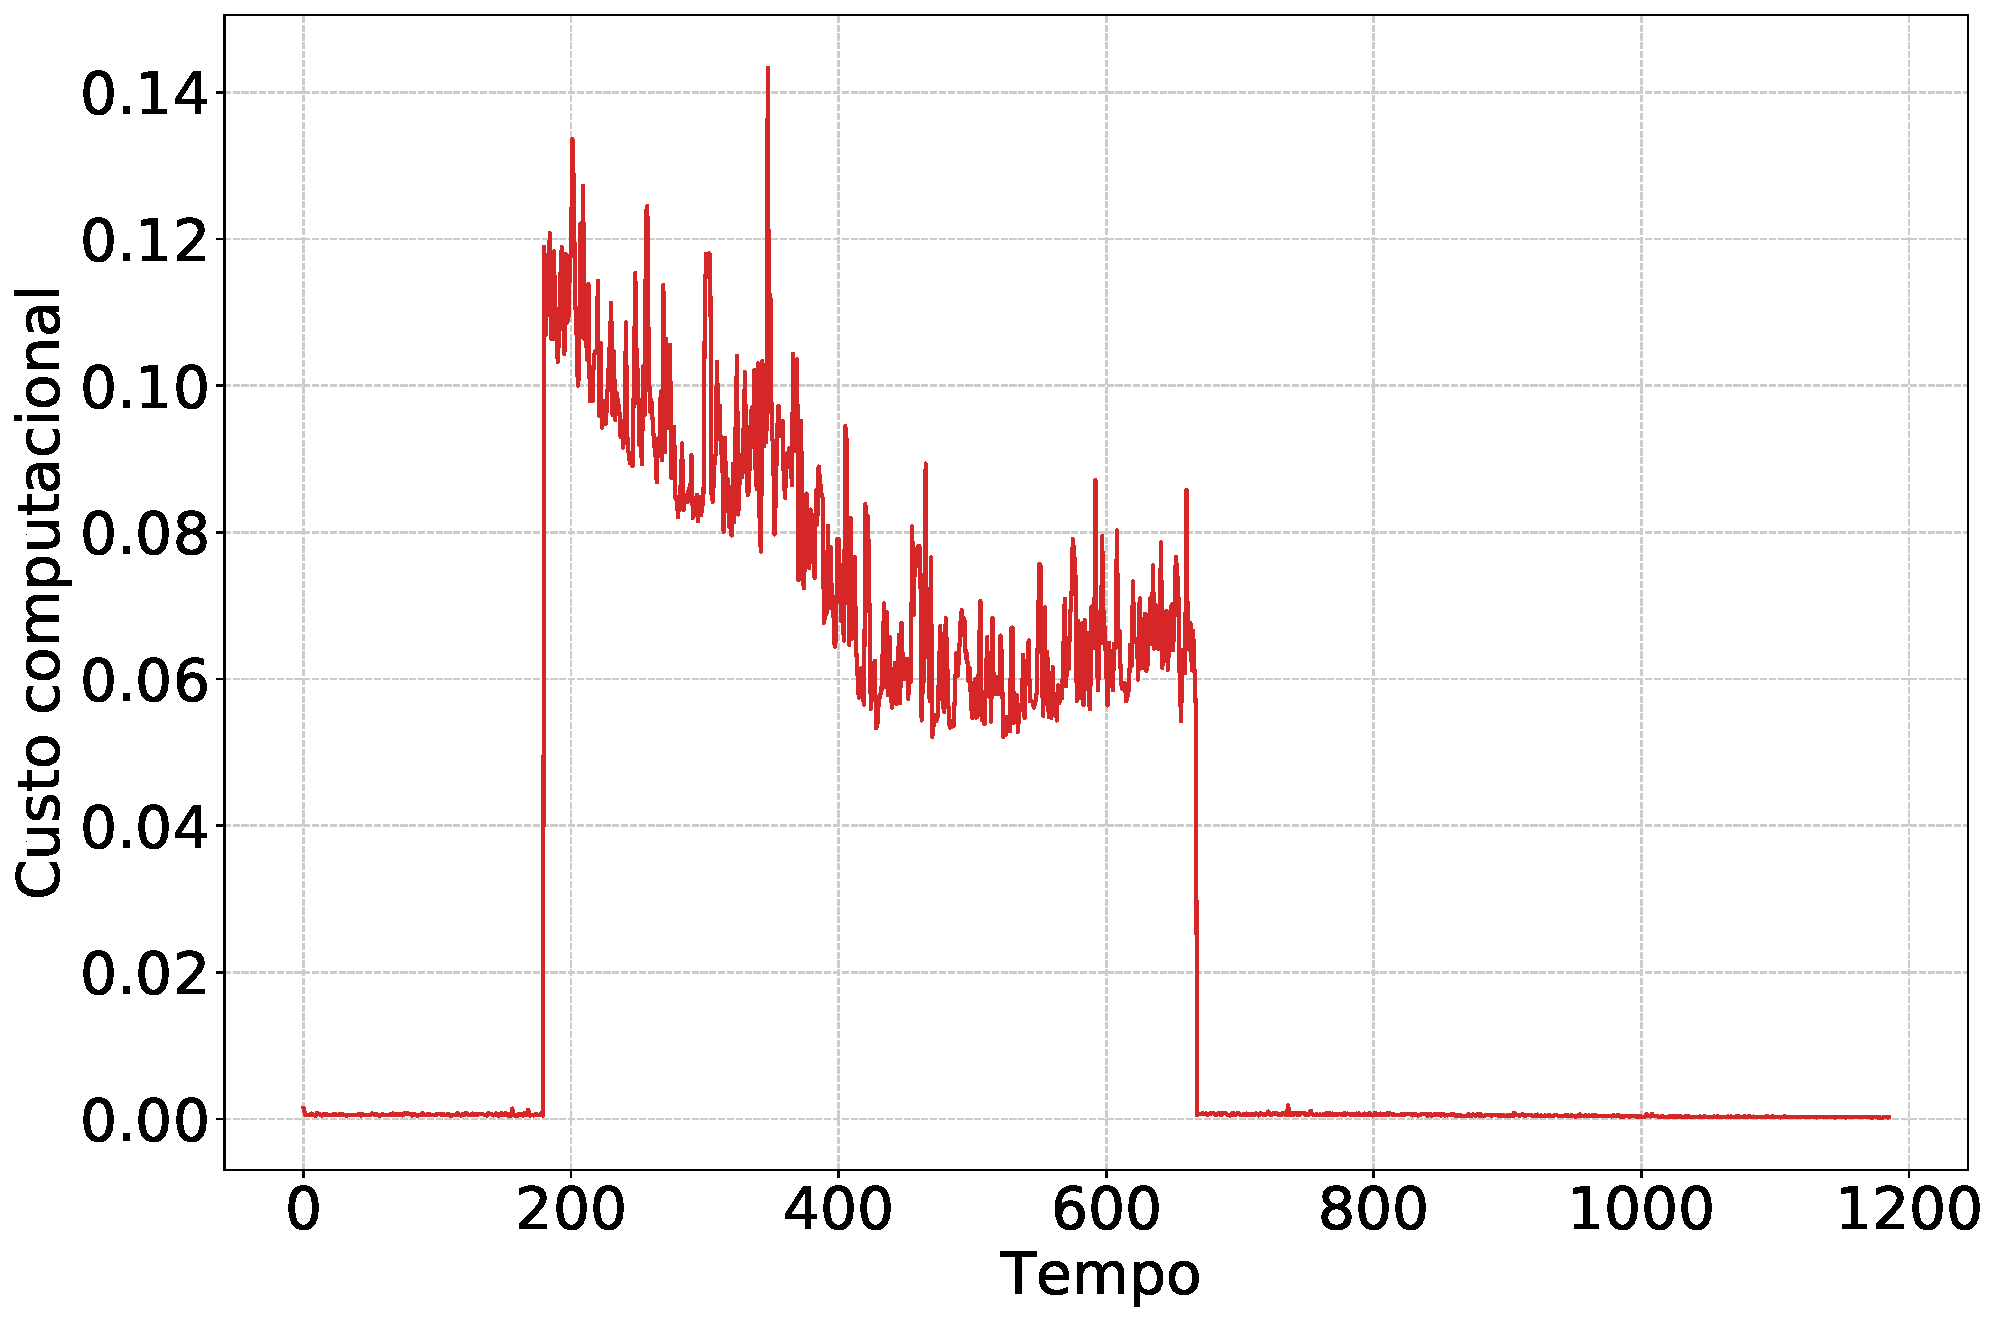
\includegraphics[width=\textwidth]{fig/chap5/crossing_right_computation_time.pdf}
            \caption{Tempo de computação}
            \label{fig:chap5_crossing_right_computation_time}
        \end{figure}
        
    \section{Crossing from Right - Embarcação Parada}
        Nessa seção apresentaremos os casos de teste onde nossa implementação se torna evidente. Realizamos novamente o caso de teste \textit{"Crossing from Right"} porém agora a outra embarcação ficará parada durante todo o teste. Esse cenário foi executado com duas configurações diferentes no sistema base: sem CPA e com CPA.
    
        \subsection{Sem CPA}
            Primeiramente apresentaremos os resultados obtidos ao executar o cenário \textit{"Crossing from Right"} com a outra embarcação parada e sem a implementação do CPA no sistema base do USV. A Figura~\ref{fig:chap5_crossing_right_stopped_vessel_no_cpa_paths} mostra o trajeto realizado pelo USV. Como pode-se observar, mesmo com a outra embarcação parada o USV tenta realizar uma manobra em conformidade com as COLREGS. Da imagem apresentada também é possível inferir que o USV não obteve sucesso na tentativa de passar por trás da outra embarcação, como requisitado pela COLREGS. Nesse caso, a distância mínima registrada durante o encontro foi de 1,352m. A Figura~\ref{fig:chap5_crossing_right_stopped_vessel_no_cpa_computation_time} mostra o tempo de computação necessário para executar a rotina apresentada no Capítulo~\ref{chap4:desenvolvimento}. Nesse caso, é possível observar um elevado esforço computacional durante quase todo o percurso, ocasionado pela criação dos obstáculos virtuais e a necessidade de planejar uma rota local. Após passar pela outra embarcação e começar a se afastar o esforço necessário diminui, dado que não é mais preciso contornar o obstáculo.
    
            \begin{figure}[H]
                \centering
                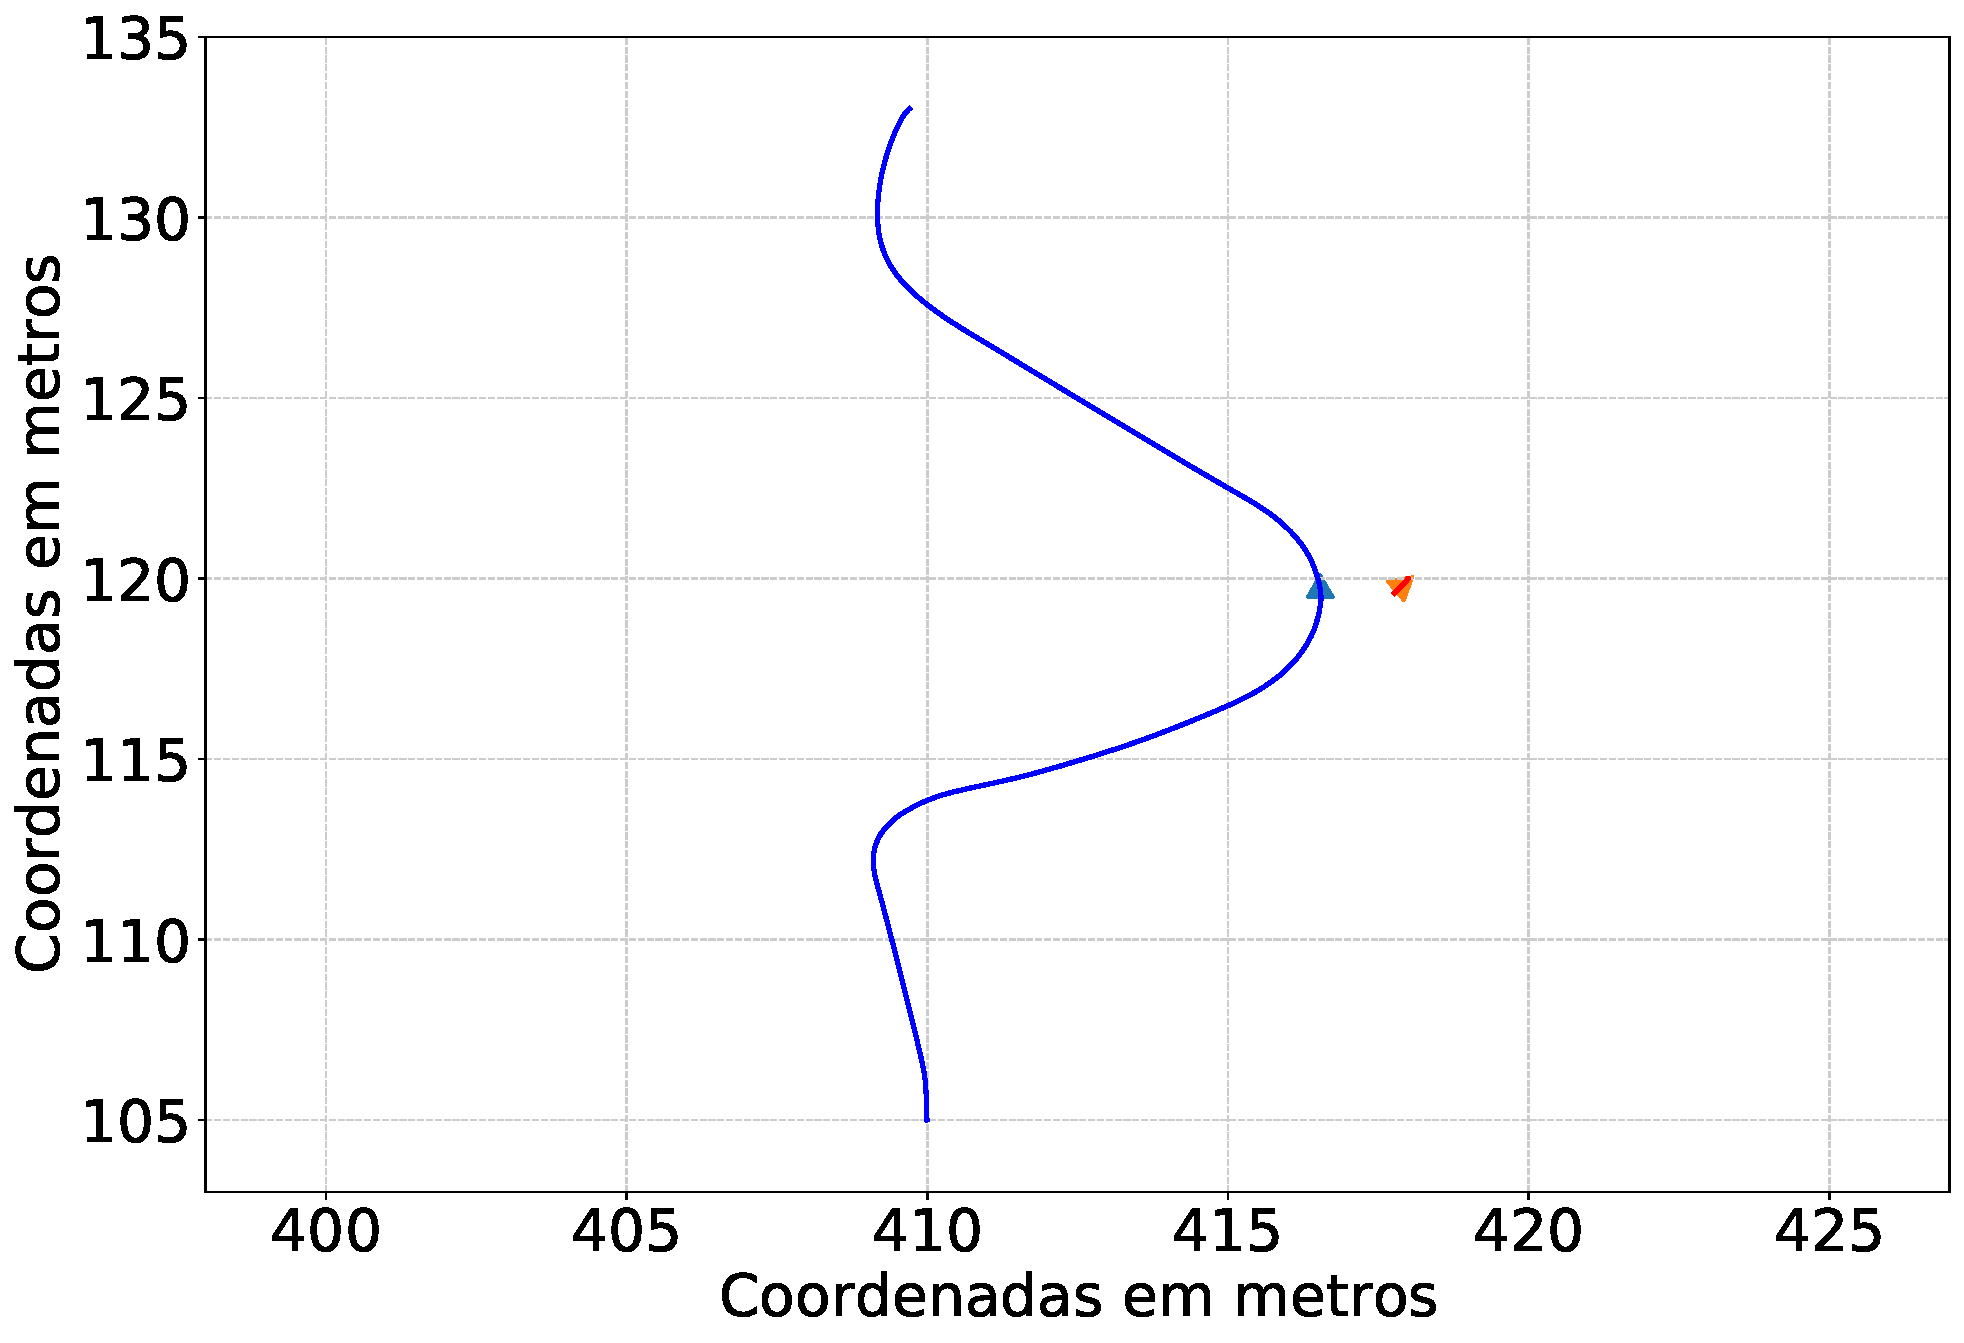
\includegraphics[scale=0.45]{fig/chap5/crossing_right_stopped_vessel_no_cpa_trajectory.pdf}
                \caption{Trajeto das embarcações}
                \label{fig:chap5_crossing_right_stopped_vessel_no_cpa_paths}
            \end{figure}
            
            \begin{figure}[H]
                \centering
                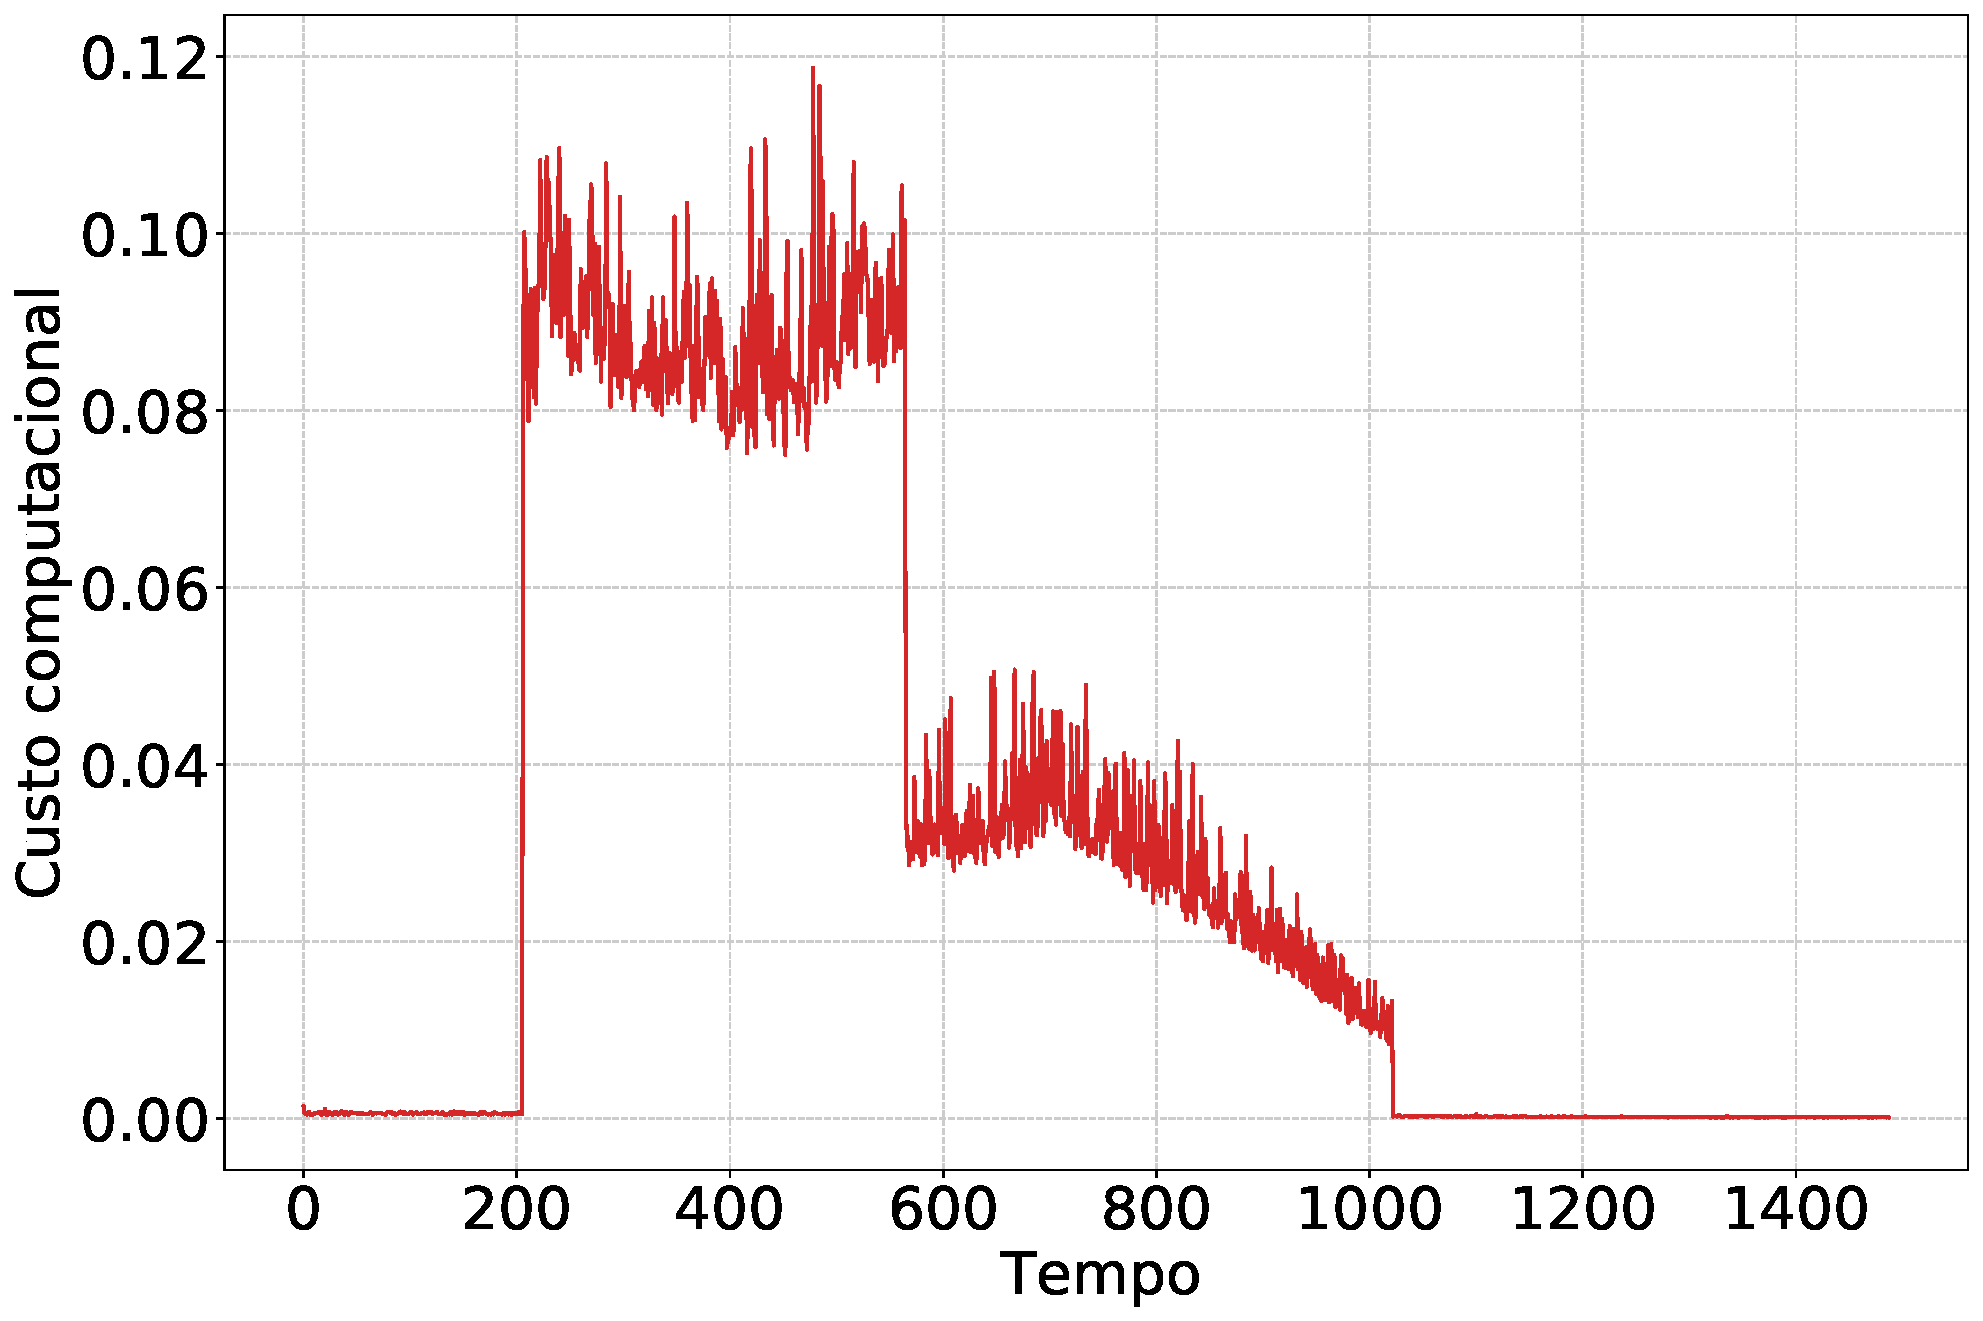
\includegraphics[scale=0.3]{fig/chap5/crossing_right_stopped_vessel_no_cpa_computation_time.pdf}
                \caption{Tempo de computação}
                \label{fig:chap5_crossing_right_stopped_vessel_no_cpa_computation_time}
            \end{figure}
            
        \subsection{Com CPA}\label{subsection_crossing_right_stopped_vessel_cpa}
            Executando o mesmo caso de teste com o CPA integrado no sistema do USV podemos observar, na Figura~\ref{fig:chap5_crossing_right_stopped_vessel_cpa_paths}, que obtivemos um resultado diferente. Novamente, a linha azul indica a rota realizada pelo USV enquanto que o triângulo vermelho indica a posição que a outra embarcação ficou durante todo o teste. O triângulo azul indica a posição do USV no momento em que a menor distância entre as embarcações foi registrada, que nesse caso foi de 10,443m. Analisando a Figura~\ref{fig:chap5_crossing_right_stopped_vessel_cpa_paths} isoladamente ficamos inclinados a entender que o CPA realizou a função desejada no sistema, indicando que não haveria risco de colisão e permitindo que o sistema realizasse o planejamento da rota local considerando a outra embarcação apenas como um obstáculo estático. Porém ao analisarmos a Figura~\ref{fig:chap5_crossing_right_stopped_vessel_cpa_computation_time} observamos que houveram dois picos de processamento durante a execução do teste. Tais picos indicam que a outra embarcação entrou no alcance do planejador local. Isso ainda não invalida o correto funcionamento do CPA, porém ao analisarmos a Figura~\ref{fig:chap5_crossing_right_stopped_vessel_cpa_tcpa} e a Figura~\ref{fig:chap5_crossing_right_stopped_vessel_cpa_dcpa}, mais precisamente entre os instantes de tempo 350 e 400, podemos inferir que a Desigualdade~\ref{eq:cpaThreshold} é satisfeita e, portanto, o sistema entende que há risco de colisão e realiza a criação de obstáculos virtuais. Isso causa uma instabilidade no sistema, fazendo com que o planejador local, por alguns instantes de tempo, determine uma rota desnecessária por consequência dos obstáculos virtuais criados. Entretanto, momentos depois o \tcpa e o \dcpa assumem valores que fazem o sistema entender que não há risco de colisão, deixando o planejador local livre para planejar a melhor rota até o objetivo. Isso faz com que o USV se afaste da outra embarcação até que ela saia do alcance do planejador local, dado que esse é um comportamento do planejador. Com a outra embarcação fora de alcance, o planejador local fica livre para determinar a rota mais curta até o objetivo, fazendo com que a outra embarcação entre novamente no alcance do planejador local, ocasionando o segundo pico de computação mostrado na Figura~\ref{fig:chap5_crossing_right_stopped_vessel_cpa_computation_time}.
        
            \begin{figure}[H]
                \centering
                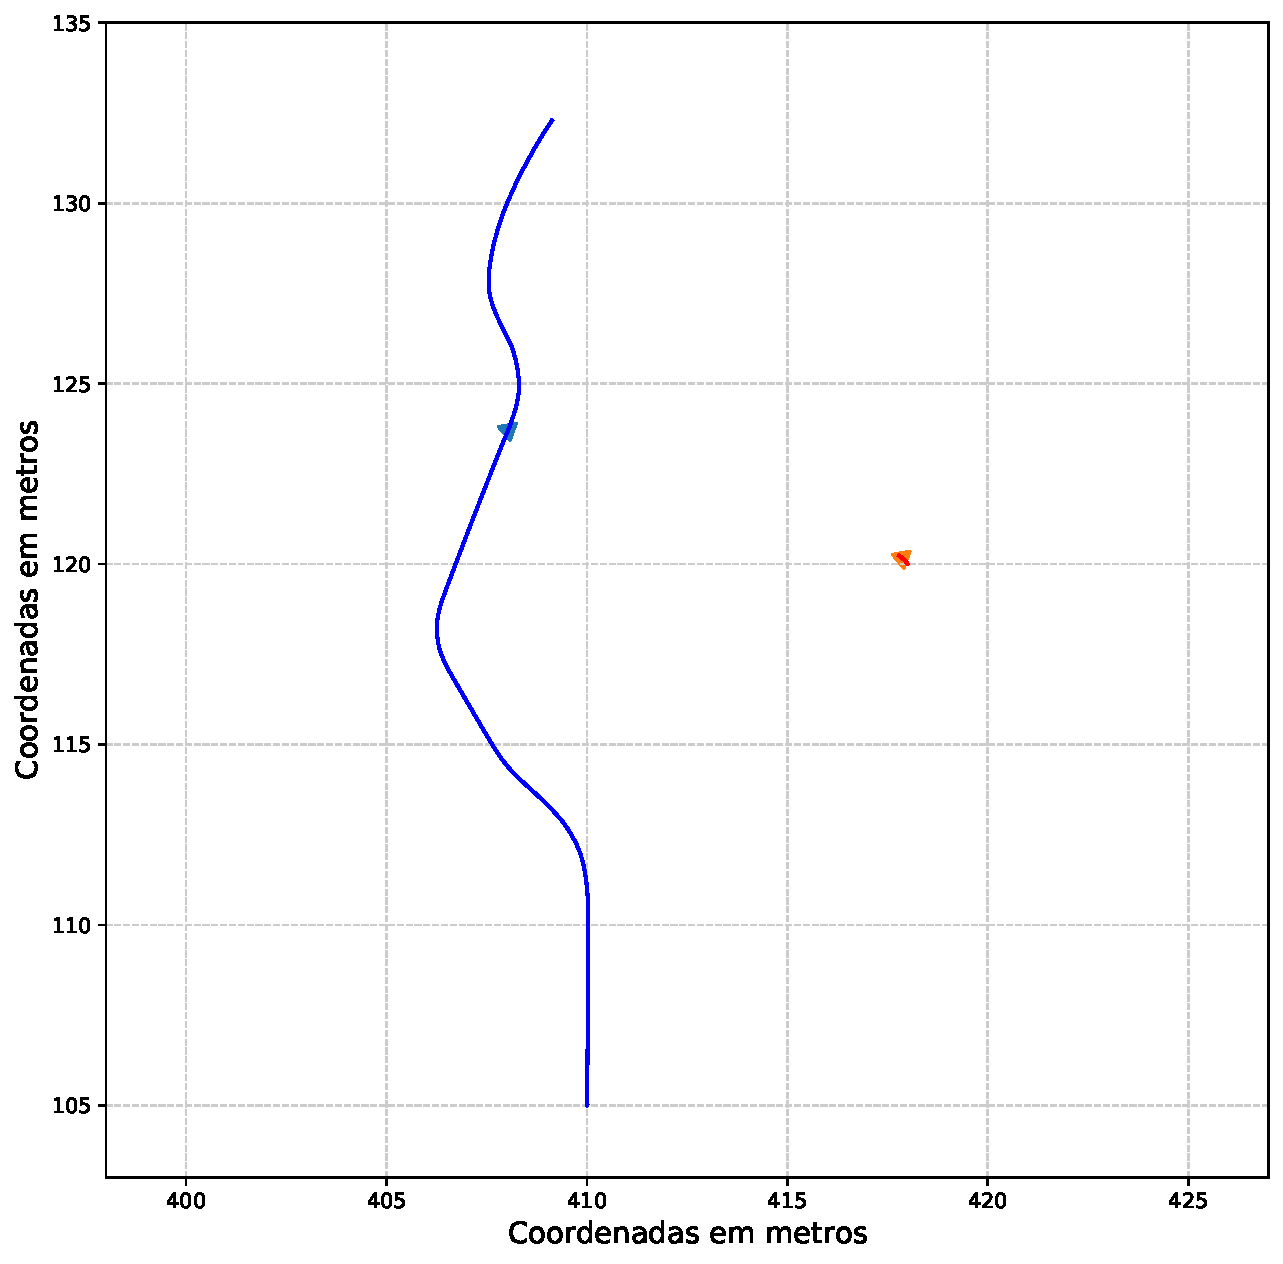
\includegraphics[scale=0.45]{fig/chap5/crossing_right_stopped_vessel_cpa_trajectory.pdf}
                \caption{Trajeto das embarcações}
                \label{fig:chap5_crossing_right_stopped_vessel_cpa_paths}
            \end{figure}
            
            \begin{figure}[H]
    		\centering
    % 		\begin{subfigure}{0.5\textwidth}
            \begin{subfigure}{1\textwidth}
                \centering
                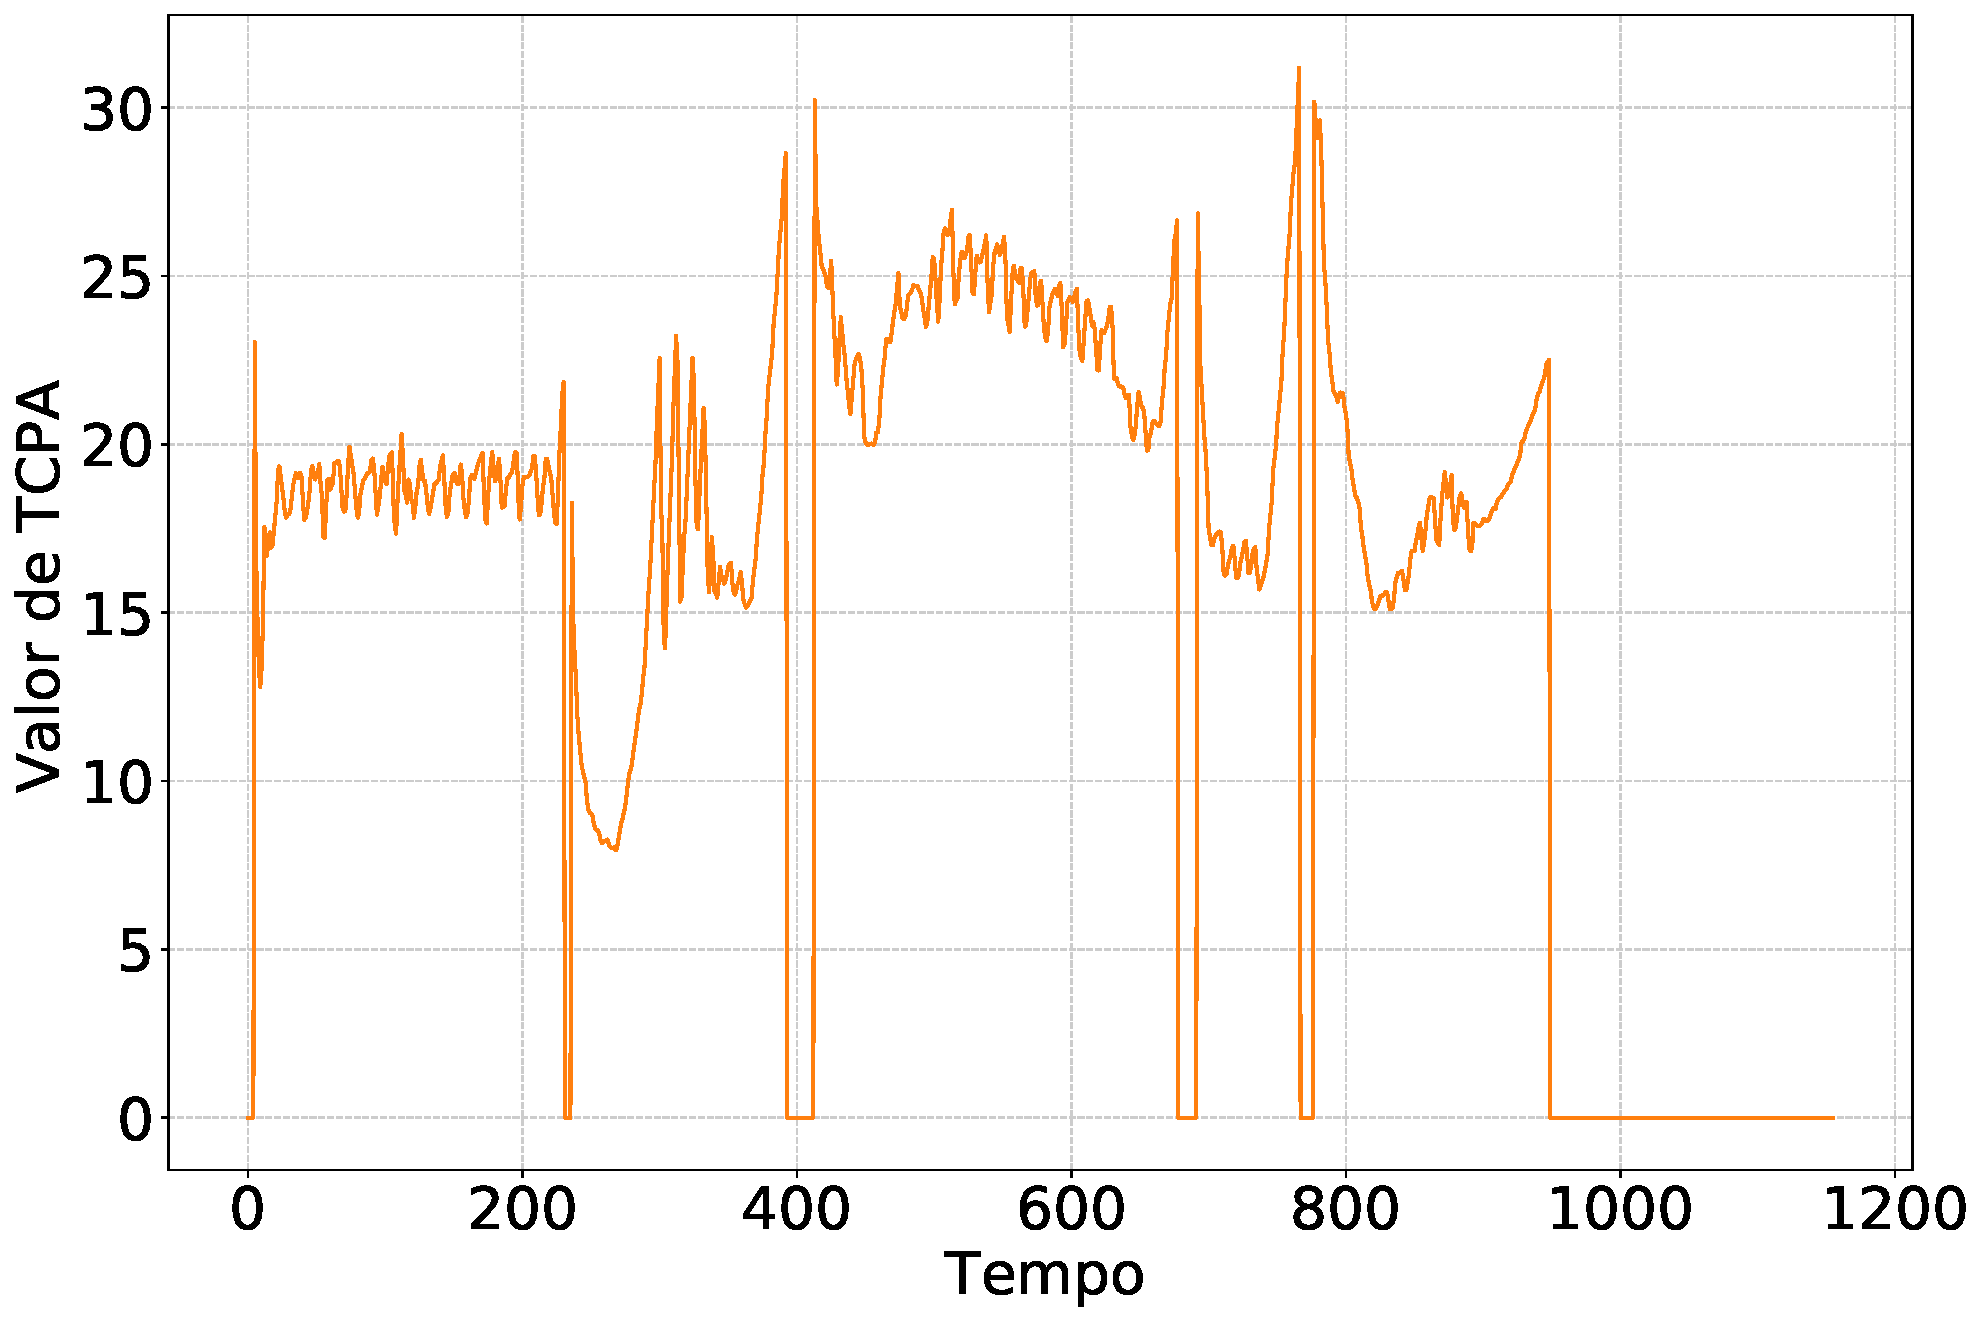
\includegraphics[width=\textwidth]{fig/chap5/crossing_right_stopped_vessel_cpa_tcpa.pdf}
                \caption{TCPA}
                \label{fig:chap5_crossing_right_stopped_vessel_cpa_tcpa}
            \end{subfigure}
            % \begin{subfigure}{0.5\textwidth}
            \begin{subfigure}{1\textwidth}
                \centering
                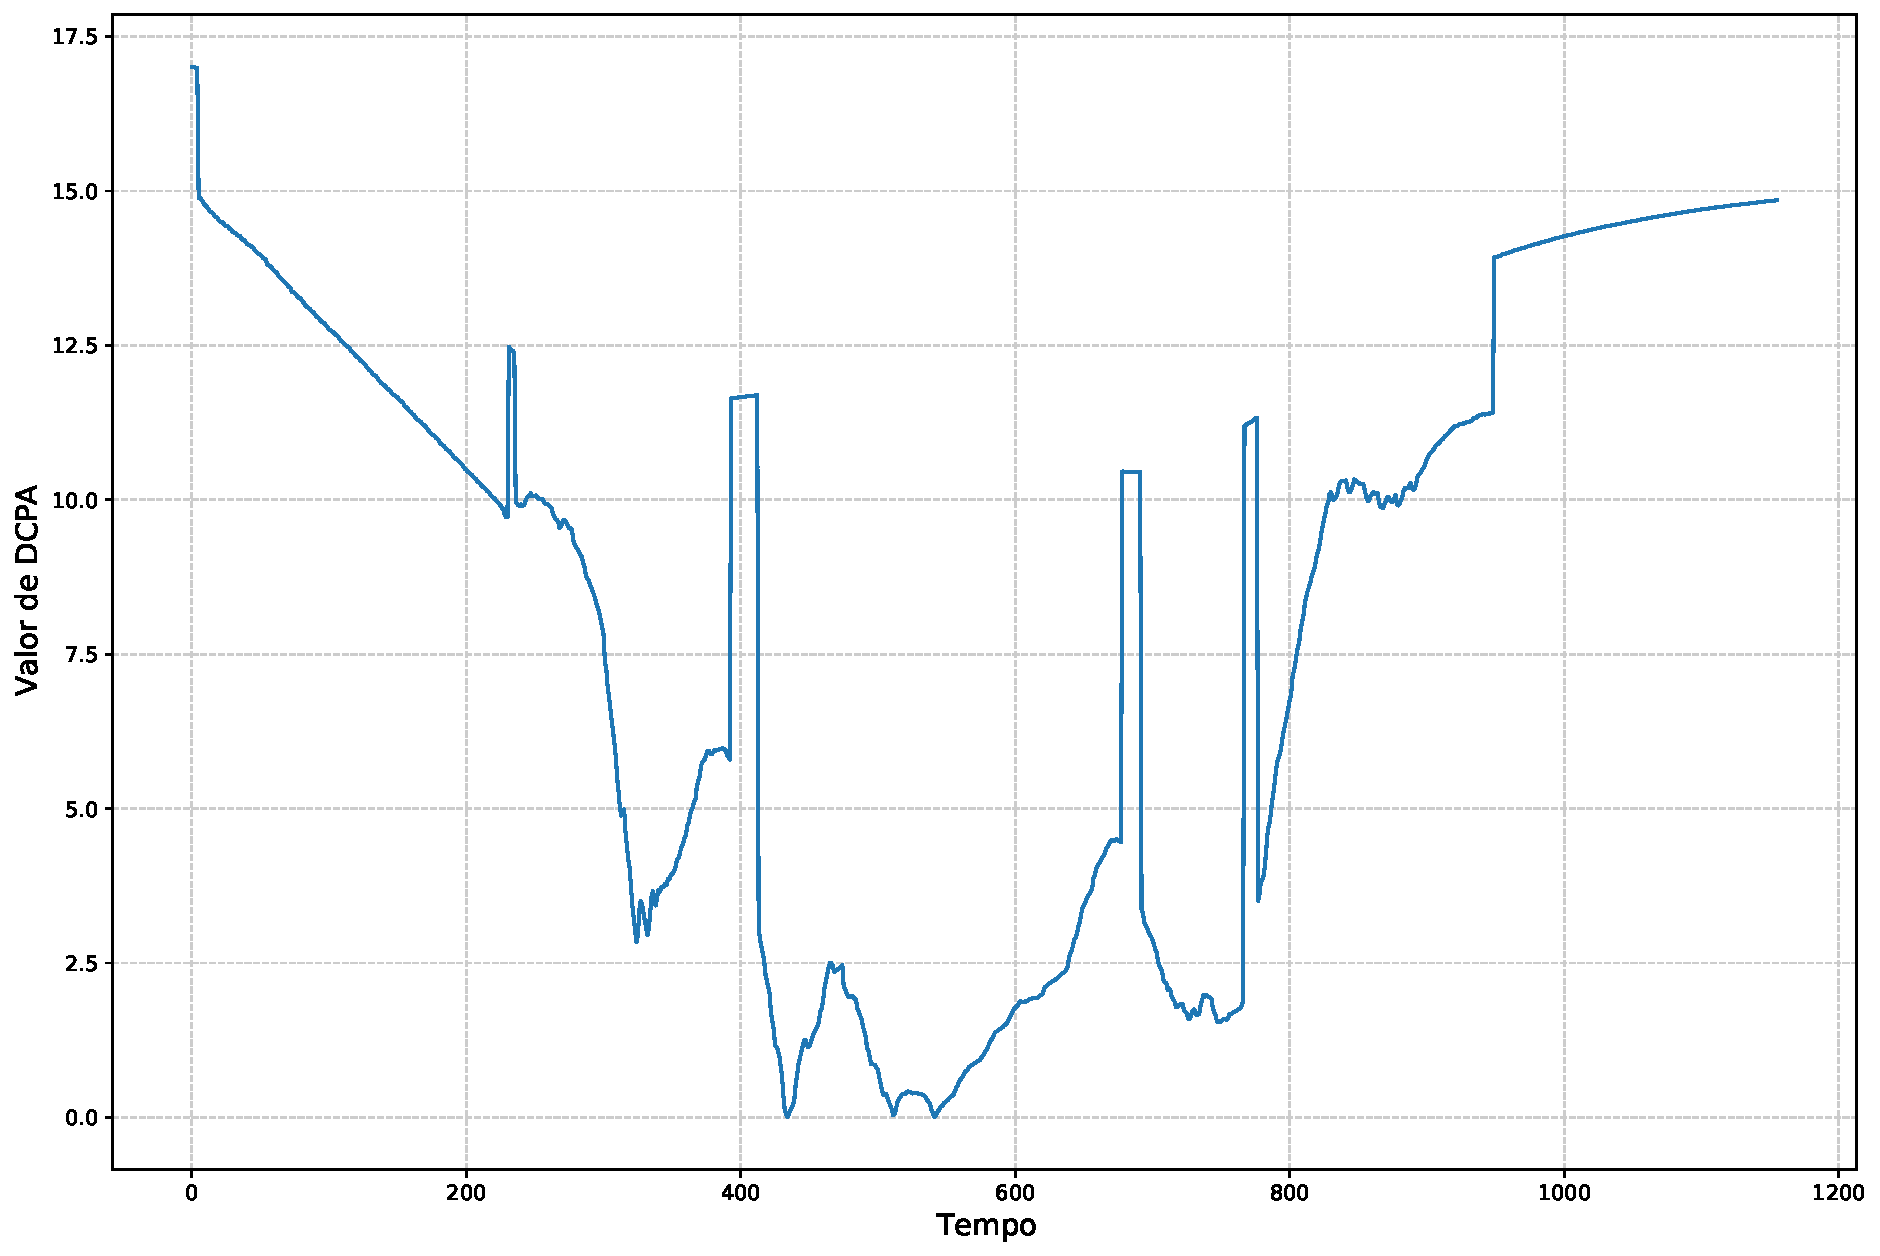
\includegraphics[width=\textwidth]{fig/chap5/crossing_right_stopped_vessel_cpa_dcpa.pdf}
                \caption{DCPA}
                \label{fig:chap5_crossing_right_stopped_vessel_cpa_dcpa}
            \end{subfigure}
            
            \caption{Informações do CPA}
            \label{fig:chap5_crossing_right_stopped_vessel_cpa}
            \end{figure}
            
            \begin{figure}[H]
                \centering
                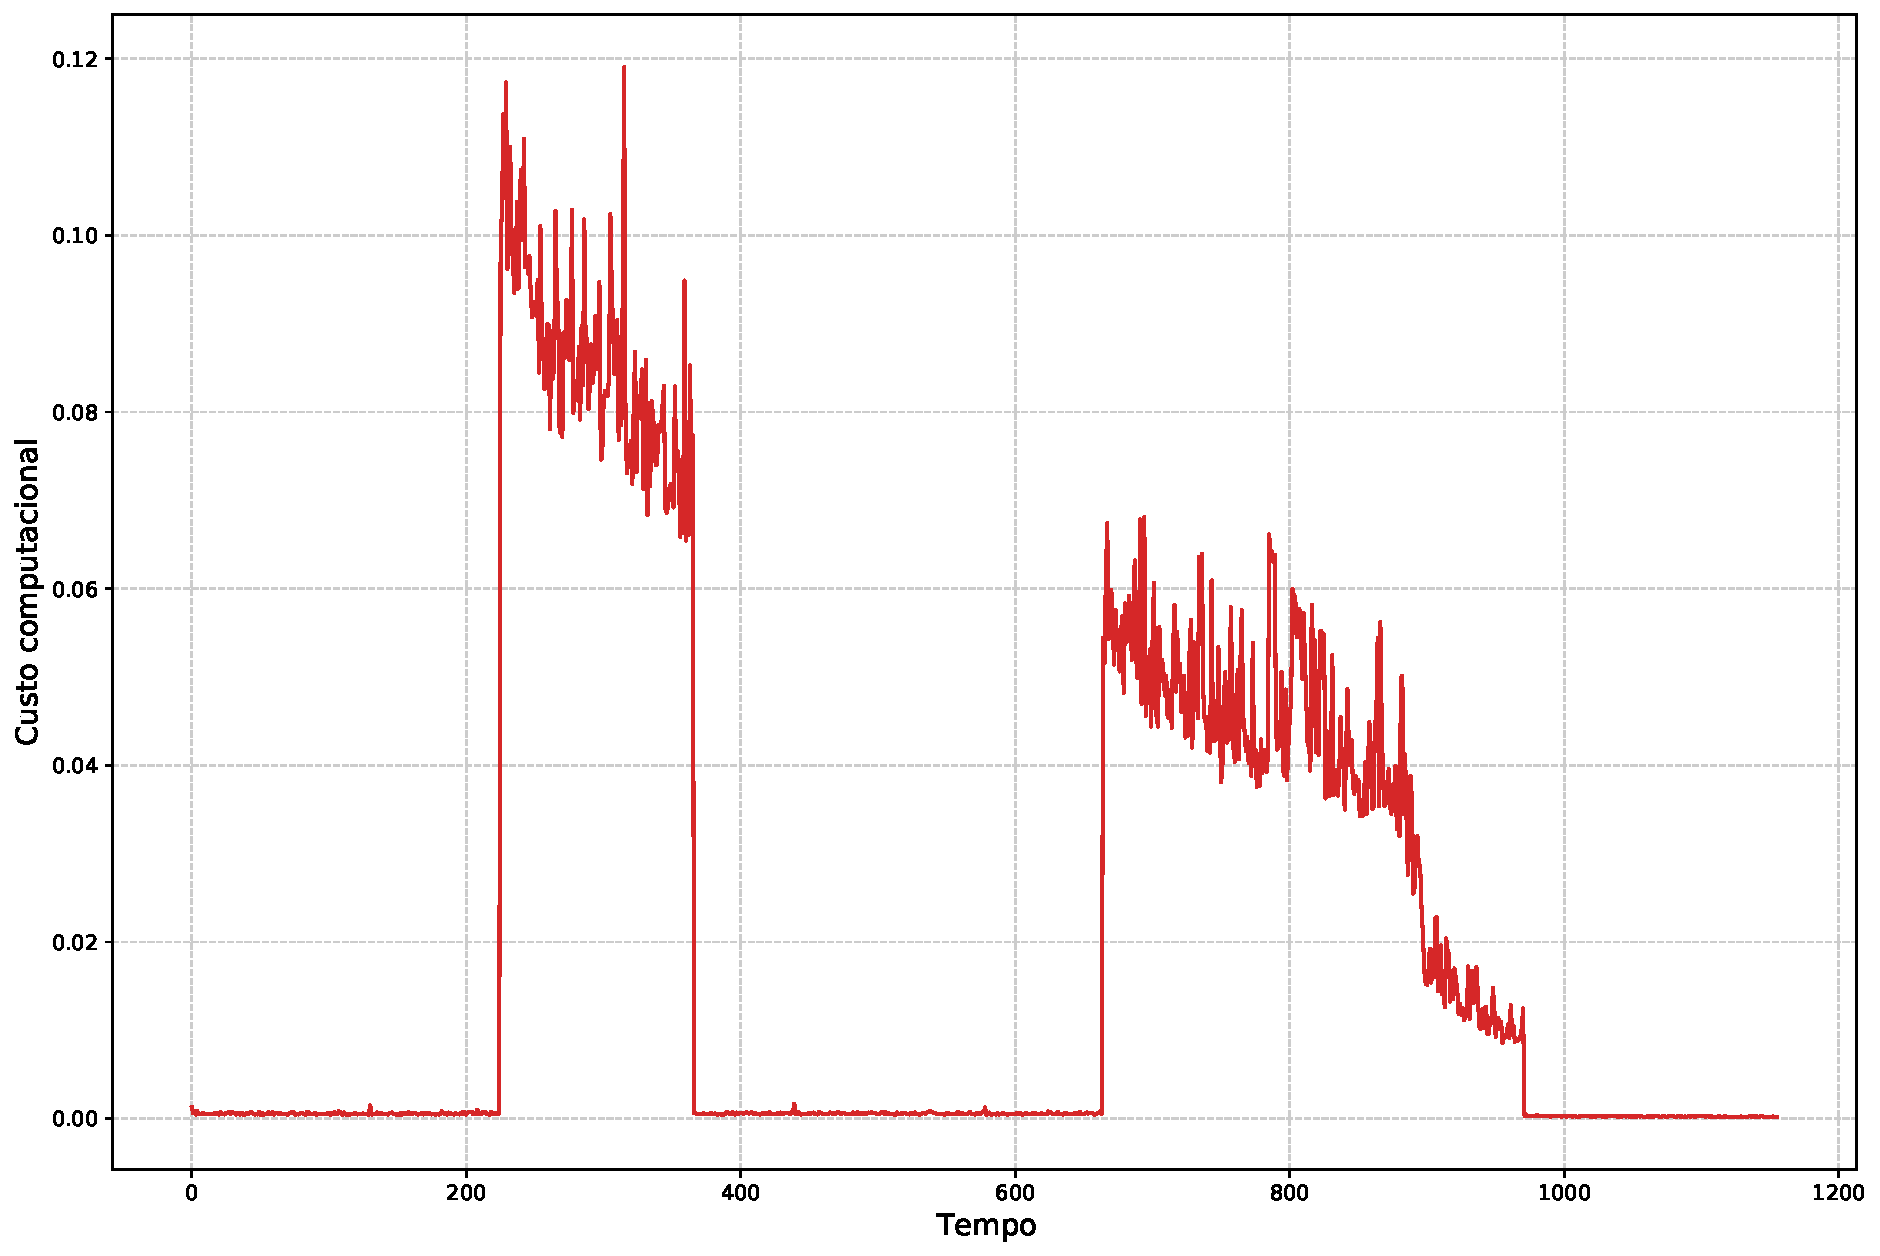
\includegraphics[width=\textwidth]{fig/chap5/crossing_right_stopped_vessel_cpa_computation_time.pdf}
                \caption{Tempo de computação}
                \label{fig:chap5_crossing_right_stopped_vessel_cpa_computation_time}
            \end{figure}
            
    \section{Comparação dos Resultados}
        Como este trabalho se propõe a contribuir com um sistema já existente, faz sentido que comparemos os nossos resultados com os de Jurak~\cite{Jurak2020COLREGS}. A Tabela~\ref{tab:chap5_comparacao_resultados} apresenta as distâncias mínimas obtidas em cada cenário por ambos os trabalhos. Como explicado na Seção~\ref{subchap5_overtake}, para o caso de teste \textit{"Overtake"} obteve-se uma distância menor que o trabalho original pois inicialmente o USV se distanciou de um objeto estático que havia em sua direita, fazendo com que ao ultrapassar a outra embarcação a distância miníma entre elas fosse menor. 
        Já no cenário \textit{"Crossing from Right"}, nossa implementação pode ter impactado para a obtenção de uma distância menor do que o trabalho original, dado que os obstáculos virtuais não são criados exatamente no momento em que o planejador local detecta a outra embarcação como no trabalho original, fazendo com que as embarcações estejam mais próximas no momento em que os obstáculos virtuais são criados. Os casos de teste \textit{"Crossing from Right"} com a outra embarcação parada não foram realizados por Jurak~\cite{Jurak2020COLREGS}, dado que seu sistema 
        não tinha o próposito de avaliar tais situações. Porém ainda assim apresentamos as menores distâncias obtidas como forma de evidenciar a nossa potencial contribuição.
        
        
        \begin{table}[]
            \centering
            \begin{tabular}{|M{5cm}|M{5cm}|M{5cm}|}
                \hline
                Cenário \textbackslash~Autor & Angnes & Jurak \\ [2ex]\hline
                Head On                      & 2,419  & 1,599 \\ [2ex]\hline
                Overtake                     & 2,255  & 3,101 \\ [2ex]\hline
                Crossing Left                & 8,316  & 6,274 \\ [2ex]\hline
                Crossing Right               & 1,866  & 3,264 \\ [2ex]\hline
                Embarcação parada sem CPA    & 1,352  & NA    \\ [2ex]\hline
                Embarcação parada com CPA    & 10,443 & NA    \\ [2ex]\hline
            \end{tabular}
            \caption{Comparação das distâncias mínimas obtidas nos trabalhos}
            \label{tab:chap5_comparacao_resultados}
        \end{table}
\chapter{Conclusão}\label{chap6:conclusao}
    Nesse capítulo apresentaremos uma síntese do trabalho realizado, discutiremos a qualidade dos resultados obtidos e os trabalhos futuros.
    
    \section{Síntese e Qualidade dos Resultados}\label{}
    % - Dizer o que foi apresentado no documento
    % - Dizer como o trabalho foi desenvolvido, citando
    % a metodologia
    % - Dizer como identificamos o problema
    % - Dizer o que foi implementado e a
    % importancia disso
    % - Dizer que nossa contribuição foi 
    % deixar o sistema base um pouco mais próximo
    % dos sistemas encontrados na literatura (todos
    % os sistemas encontrados na literatura possuiam
    % CPA implementado)
    % - Dizer que o cálculo do CPA precisa ser revisado,
    % pois o modo como Kuwata equacionou pode não ser
    % aplicável para o nosso sistema
        Nesse trabalho apresentamos a melhoria de um sistema para veículos de superfície não tripulados (do inglês \textit{"Unmanned Surface Vehicle"} - USV) já existente, realizando a implementação do ponto de maior proximidade (do inglês \textit{"Closest Point of Approach"} - CPA), onde buscamos explorar a oportunidade de realizar um trabalho seguindo uma metodologia científica. Ao comparar o sistema desenvolvido por Jurak~\cite{Jurak2020COLREGS} com a literatura (trabalhos realizados por Kuwata~\etal~\cite{Kuwata2014Safe}, Huang~\etal~\cite{Huang2019Generalized} e Song~\etal~\cite{Song2018Two-level}) percebemos que uma das diferenças era a falta do CPA no sistema de Jurak~\cite{Jurak2020COLREGS}, e optamos por atacar esse ponto. 
        
        Os cálculos necessários para a determinação do CPA tiveram como base teórica o trabalho realizado por Kuwata~\etal~\cite{Kuwata2014Safe}. Dado que as posições e velocidades das embarcações eram informações já utilizadas pelo sistema de Jurak~\cite{Jurak2020COLREGS}, fizemos uso das mesmas para realizar o cálculo do CPA. Realizamos os cálculos necessários de forma relativamente simples, porém a 
        alteração realizada no sistema base para faze-lo considerar o CPA demandou grande esforço, pois tal implementação não deveria comprometer o funcionamento atual do sistema base. 
        
        Como indicado pelos resultados dos testes, conseguimos preservar o funcionamento do sistema base e adicionamos a implementação do CPA. Porém, como apresentado na Seção~\ref{subsection_crossing_right_stopped_vessel_cpa}, em uma situação em que não há risco de colisão, a nossa implementação do CPA pode indicar que há risco de colisão. Isso poderia ser resolvido alterando os limiares da Desigualdade~\ref{eq:cpaThreshold}, porém isso demandaria mais tempo de testes, análises e entendimento dos resultados. Dado o curto tempo de implementação do trabalho, optamos por manter os resultados que obtivemos até então como prova que o conceito do CPA está funcional para determinadas situações. Entretanto, não houveram ocorrências em nossos testes para a situação inversa, em que o CPA informaria que não há risco de colisão em uma situação de risco eminente. 
    
    \section{Trabalhos Futuros}
    
        Para continuação deste trabalho é necessário compreender a razão pela qual houve detecção de risco de colisão quando na verdade não havia. Uma das possibilidades citadas na seção anterior é a alteração dos valores a serem atingidos pelo \tcpa e \dcpa para ser detectado o risco de colisão. Porém, pode ser preciso ter um maior entendimento se a equação apresentada por Kuwata~\etal~\cite{Kuwata2014Safe} é aplicável ao sistema desenvolvido por Jurak~\cite{Jurak2020COLREGS}. Por exemplo, no escopo deste trabalho, assumimos que o valor absoluto do \tcpa encontrado deveria ser usado, desconsiderando resultados negativos, visto que inverteria o sentido da velocidade das embarcações. Kuwata~\etal~\cite{Kuwata2014Safe} 
        não faz menção sobre usar o valor absoluto ou não. Também seria preciso entender se o equacionamento apresentado por Kuwata~\etal~\cite{Kuwata2014Safe} é aplicável a curtas distâncias e baixas velocidades, visto que em seus testes o objetivo do USV estava a 1000m de distância e ele se deslocava a uma velocidade de 4m/s. No nosso caso, objetivos para nosso USV eram definidos a pouco mais de 10m de distância da posição inicial com um deslocamento médio de 0,5m/s.
\include{tcc_final_cap7}

%----------------------------------------------------------------
% Aqui vai a bibliografia. Existem 3 estilos de citação: use
% 'tcc-alpha' para citações do tipo [Abc+] ou [XYZ] (em ordem
% alfabética na bibliografia), 'tcc-num' para citações
% numéricas do tipo [1], [20], etc., em ordem de referência e
% 'tcc-alpha-full' para citações estilo 'alpha' mas com nomes completos.
%----------------------------------------------------------------
%\bibliographystyle{tcc-alpha}
\bibliographystyle{tcc-num}
\bibliography{tcc_final_bib}

%----------------------------------------------------------------
% Após \appendix, se iniciam os capítulos de Apêndice, com
% numeração alfabética.
%----------------------------------------------------------------
%\appendix
%\chapter{Meu primeiro apêndice}
%\chapter{My second appendix}

%----------------------------------------------------------------
% Aqui vão os "capítulos" de anexos. Cada anexo deve
% ser considerado um capítulo.
%----------------------------------------------------------------
%\anexos
%\chapter{Meu primeiro anexo}
%\chapter{My second attachment}

% E aqui (para a felicidade de todos) termina o documento.
\end{document}
